%===============================================================
% Template using official colors of Czech Technical University.
% They are defined by new graphical manual - 2017.
% Specially designed for Laboratory of Structure of Biomolecules
% Share and modify as you like. Keep the name of the author.
% It is forbidden to use the template commercially.
% Author: Martin Malý.
% Published: 23.9.2017.
%===============================================================

\documentclass{beamer}
\usepackage[utf8]{inputenc}

\usetheme{Madrid}
  
\definecolor{cvut_navy}{HTML}{0065BD}
\definecolor{cvut_blue}{HTML}{6AADE4}
\definecolor{cvut_gray}{HTML}{156570}

\usepackage{xcolor}
\definecolor{azulUC3M}{RGB}{0,0,102}
\definecolor{gray97}{gray}{.97}
\definecolor{gray75}{gray}{.75}
\definecolor{gray45}{gray}{.45}

\setbeamercolor{section in toc}{fg=black,bg=white}
\setbeamercolor{alerted text}{fg=gray45}
\setbeamercolor*{palette primary}{bg=azulUC3M,fg=gray!20!white}
\setbeamercolor*{palette secondary}{bg=gray45,fg=white}
\setbeamercolor*{palette tertiary}{parent=palette primary}
\setbeamercolor*{palette quaternary}{fg=green,bg=gray!5!white}

\setbeamercolor*{sidebar}{fg=azulUC3M,bg=gray!15!white}


\setbeamercolor{titlelike}{parent=palette primary}
\setbeamercolor{frametitle}{parent=palette primary}

\setbeamercolor*{separation line}{}
\setbeamercolor*{fine separation line}{}

\setbeamertemplate{navigation symbols}{} 


\usepackage{eqnarray,amsmath}
\usepackage{amsfonts}
\usepackage{amssymb}
\usepackage{graphicx}
\usepackage{lmodern} % pro pismo tucne a zaroven kurziva
\usepackage{bm} % pro pismo tucne a zaroven kurziva
\usepackage{epstopdf}
\usepackage{changepage}
\usepackage{array,booktabs}

% definice makra pro české uvozovky:
\def\bq{\mbox{\kern.1ex\protect\raisebox{-1.3ex}[0pt][0pt]{''}\kern-.1ex}}
\def\eq{\mbox{\kern-.1ex``\kern.1ex}}
\def\ifundefined#1{\expandafter\ifx\csname#1\endcsname\relax }%
\ifundefined{uv}%
        \gdef\uv#1{\bq #1\eq}
\fi
% konec .... použití makra pro psaní český uvozovek: \uv{text uvnitř uvozovek}





% DATOS
\author[J. M. Espinosa Moral]{Juan Manuel Espinosa Moral\\
Tutor/es: Ana García Armada}
\institute[UC3M]{
	Universidad Carlos III de Madrid \\
	Av. de la Universidad, 30, 28911. Leganés, Madrid
}
\title[Emulación realista del acceso radio 5G]{Emulación realista del acceso radio 5G}
\subtitle{Trabajo Fin de Máster}
\date[MUIT]{
	Máster Universitario en Ingeniería de Telecomunicación\\
	22 de septiembre de 2026}
% \logo{\includegraphics[height=1cm]{overleaf-logo}}





% OTRA CONFIGURACIÓN

% Muestra los contenidos al principio de cada seccción
\AtBeginSection[]
{
	\begin{frame}
		\frametitle{Contenido de la sección}
		\tableofcontents[currentsection]
	\end{frame}
}





%====================================================
%========== BEGINNING OF DOCUMENT ===================
%====================================================

\begin{document}





% PORTADA

% Diapositiva
\begin{frame}
	\titlepage

	\begin{center}
		
\includegraphics[height=1.6cm]{../memoria/imagenes/Logo_UC3M.svg.png}
	\end{center}
\end{frame}

% Logo de las esquinas a partir de la portada
\logo{
\includegraphics[height=1cm]{../memoria/imagenes/Acronimo_nombre3l.jpg}}

% Diapositiva
\begin{frame}
	\frametitle{Contenido}

	\tableofcontents
\end{frame}





% SECCIÓN
\section{Introducción}

% SUBSECCIÓN
\subsection{Motivaciones}

% Diapositiva
\begin{frame}
\frametitle{Motivaciones (I)}

\begin{columns}[onlytextwidth]
\begin{column}{0.7\textwidth}
\begin{itemize}
\item {
	Quinta generación de comunicaciones móviles (5G).
	\begin{itemize}
	\item \textit{3rd Generation Partnership Project} (3GPP).
	\item Casos de uso.
	\item {
		Desarrollo de aplicaciones.
		\begin{itemize}
		\item Despliegues existentes.
		\item Exhaustivos ensayos y metodologías fiables.
		\end{itemize}
	}
	\item {
		Desarrollo de los despliegues.
		\begin{itemize}
		\item Ajuste de varios elementos.
		\item Interfaz de radio de 5G (NR).
		\end{itemize}
	}
	\end{itemize}
}
\end{itemize}
\end{column}

\begin{column}{0.3\textwidth}
\begin{center}
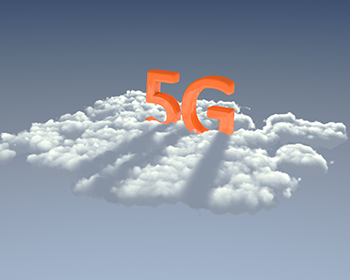
\includegraphics[height=2.0cm]{../memoria/imagenes/3gpp_5g_system_overview/5g-system-overview03.png}

\vspace{1.0cm}


\includegraphics[height=1.5cm]{../memoria/imagenes/3gpp/Logo_3GPP.svg.png}
\end{center}
\end{column}
\end{columns}
\end{frame}

% Diapositiva
\begin{frame}
\frametitle{Motivaciones (II)}

\begin{itemize}
\item {
	Nuevos casos de uso.
	\begin{itemize}
	\item XR, VR, AR. $\rightarrow$ Baja latencia.
	\item Comunicaciones en entornos vehiculares (C-V2X). $\rightarrow$ Baja latencia.
	\item Inconvenientes para cobre, fibra óptica, cable coaxial, etc. $\rightarrow$ Cobertura de gran ancho de banda.
	\end{itemize}
}
\end{itemize}

\begin{center}
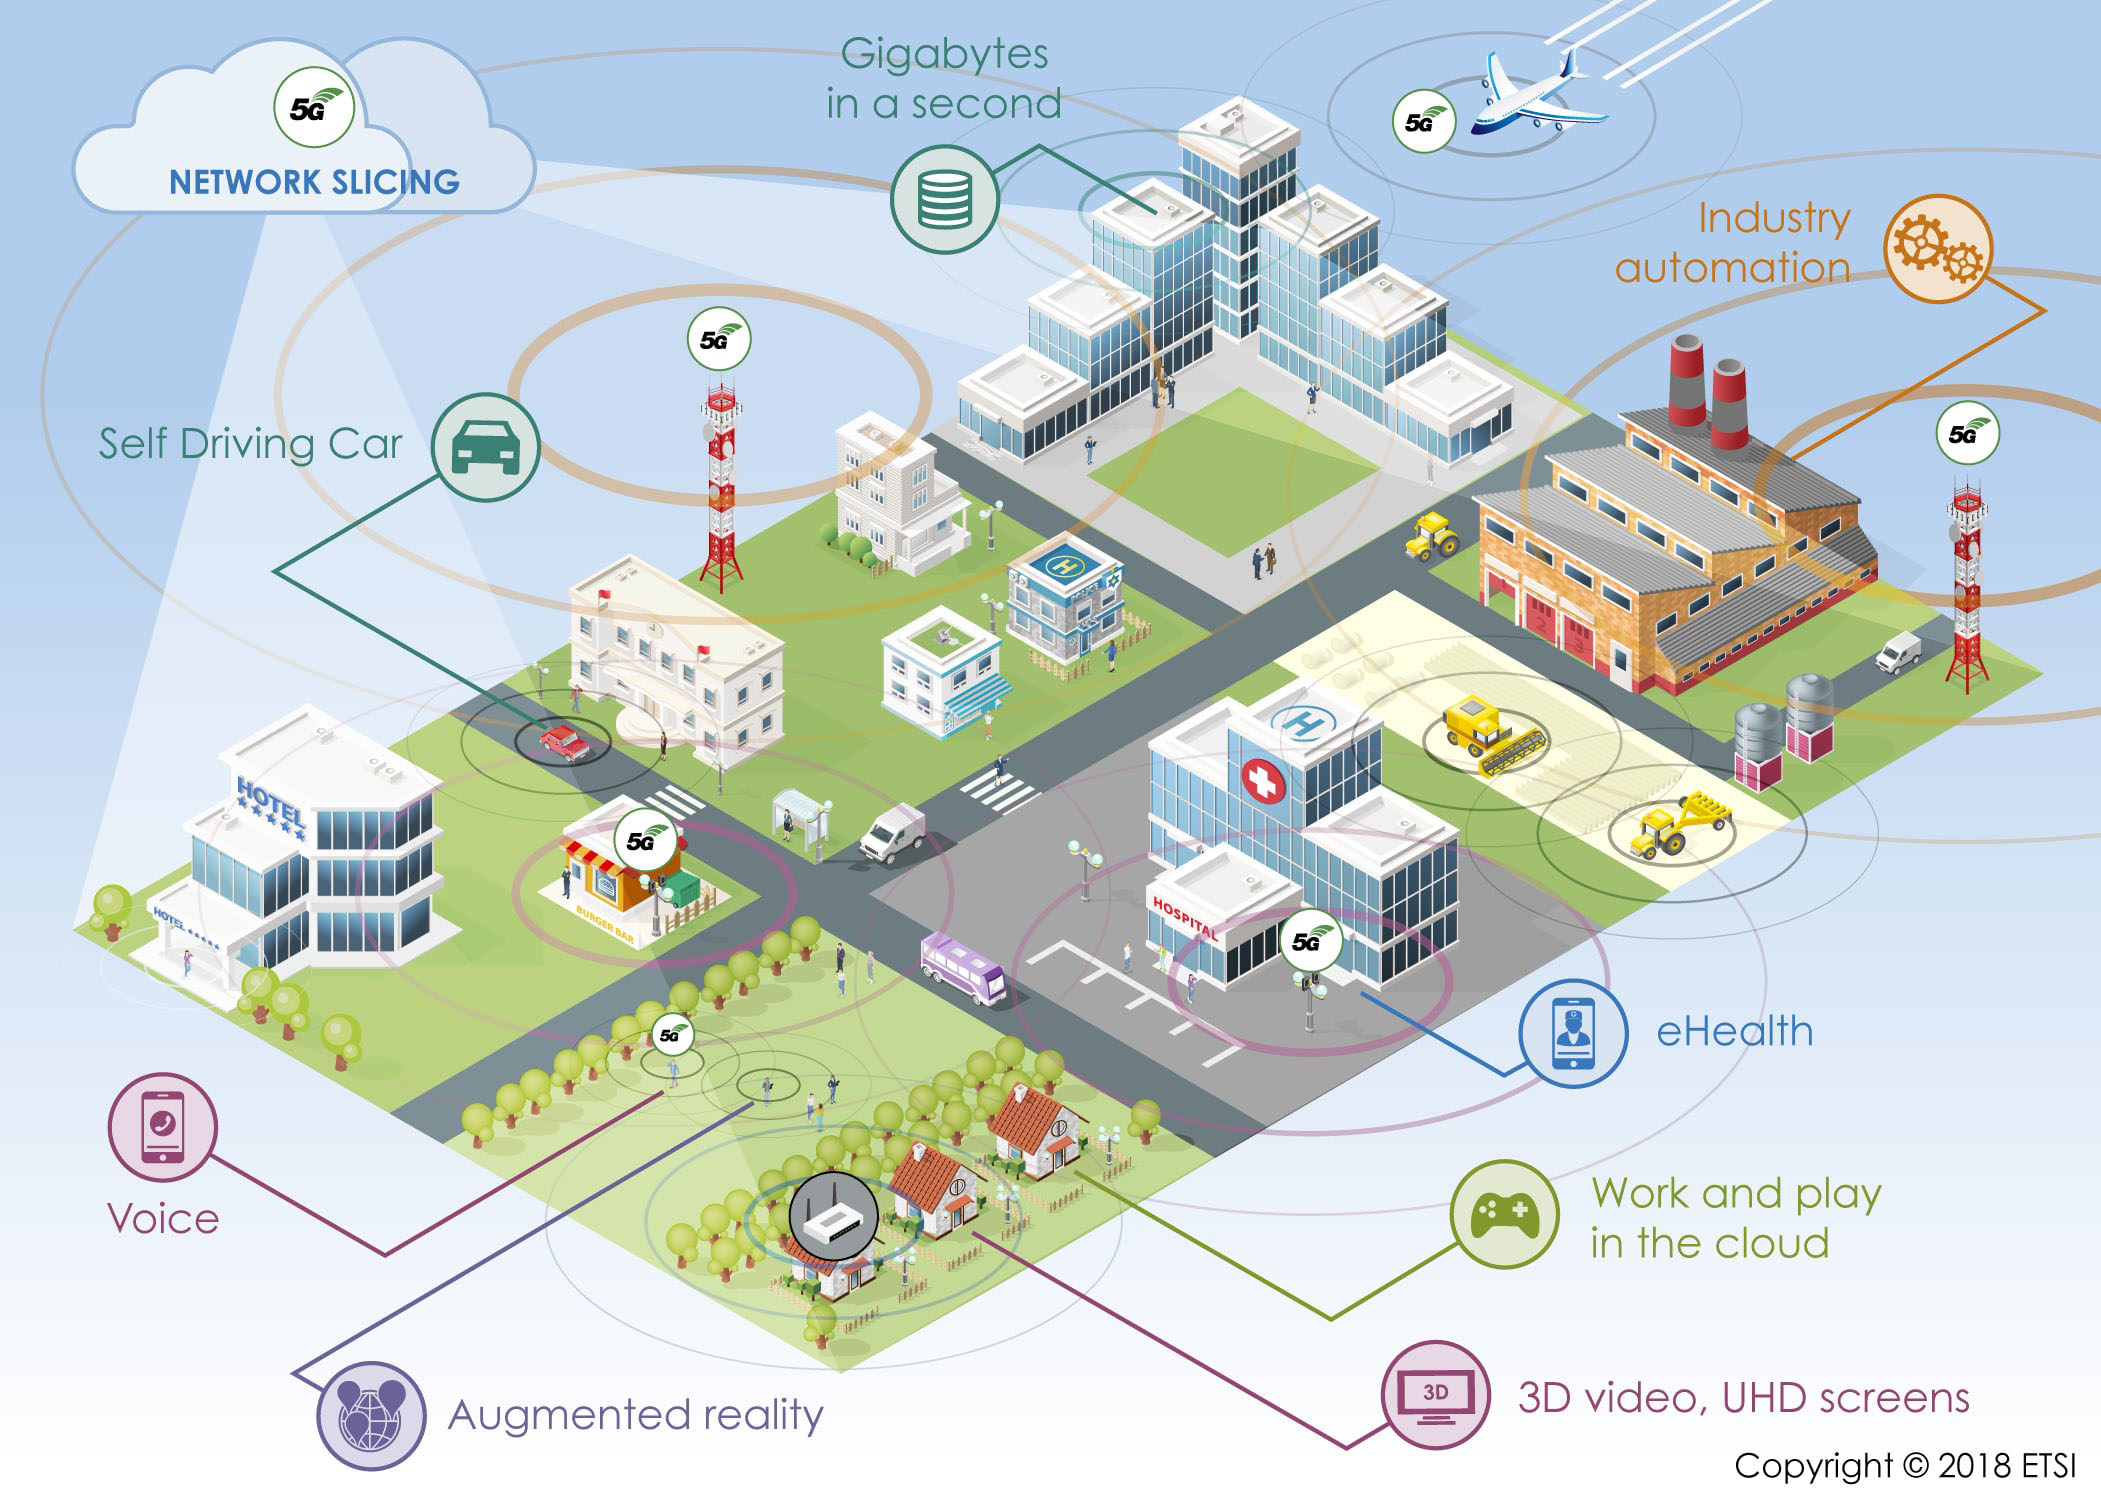
\includegraphics[height=5.0cm]{../memoria/imagenes/etsi_5g/5G_use_cases_ETSI_illustration.jpg}
\end{center}
\end{frame}

% SUBSECCIÓN
\subsection{Estado de la cuestión}

% Diapositiva
\begin{frame}
\frametitle{Estado de la cuestión (I)}

\begin{columns}[onlytextwidth]
\begin{column}{0.7\textwidth}
\begin{itemize}
\item {
	Simuladores de RAN.
	\begin{itemize}
	\item Probar configuraciones de red.
	\item Diseñar tras acotar unas prestaciones.
	\end{itemize}
}
\item {
	Emuladores de RAN.
	\begin{itemize}
	\item Probar configuraciones de red.
	\item Diseñar tras acotar unas prestaciones.
	\item Probar aplicaciones para 5G que se ejecutan en tiempo real.
	\end{itemize}
}
\end{itemize}
\end{column}

\begin{column}{0.3\textwidth}
\begin{center}

\includegraphics[height=0.8cm]{../memoria/imagenes/emuladores/5G-lena-logo.png}

\includegraphics[height=0.8cm]{../memoria/imagenes/emuladores/matlab_5g_toolbox_logo.png}

\vspace{0.5cm}


\includegraphics[height=0.8cm]{../memoria/imagenes/emuladores/hero-banner.png}

\vspace{0.5cm}


\includegraphics[height=0.5cm]{../memoria/imagenes/emuladores/keysight_logo.png}

\vspace{0.5cm}


\includegraphics[height=0.4cm]{../memoria/imagenes/emuladores/ns-3-notext.png}

\vspace{0.5cm}


\includegraphics[height=0.5cm]{../memoria/imagenes/emuladores/open_ait_interface_logo.png}
\end{center}
\end{column}
\end{columns}
\end{frame}

% Diapositiva
\begin{frame}
\frametitle{Estado de la cuestión (II)}

\begin{columns}[onlytextwidth]
\begin{column}{0.7\textwidth}
\begin{itemize}
\item {
	Emulador \textit{FikoRE}.
	\begin{itemize}
	\item Desarrollada por \textit{Nokia} en colaboración con la UC3M.
	\item Experimentación a nivel de aplicación.
	\item Usuarios de distintas disciplinas pueden utilizarlo.
	\item Permite su modificación de manera sencilla.
	\item {
		Buenas prestaciones a nivel de
		\begin{itemize}
		\item tráfico soportado.
		\item número de instancias.
		\item escalabilidad.
		\item precisión.
		\end{itemize}
	}
	\item Permite analizar casos de uso y despliegues de red con un alto nivel de realismo.
	\end{itemize}
}
\end{itemize}
\end{column}

\begin{column}{0.3\textwidth}
\begin{center}
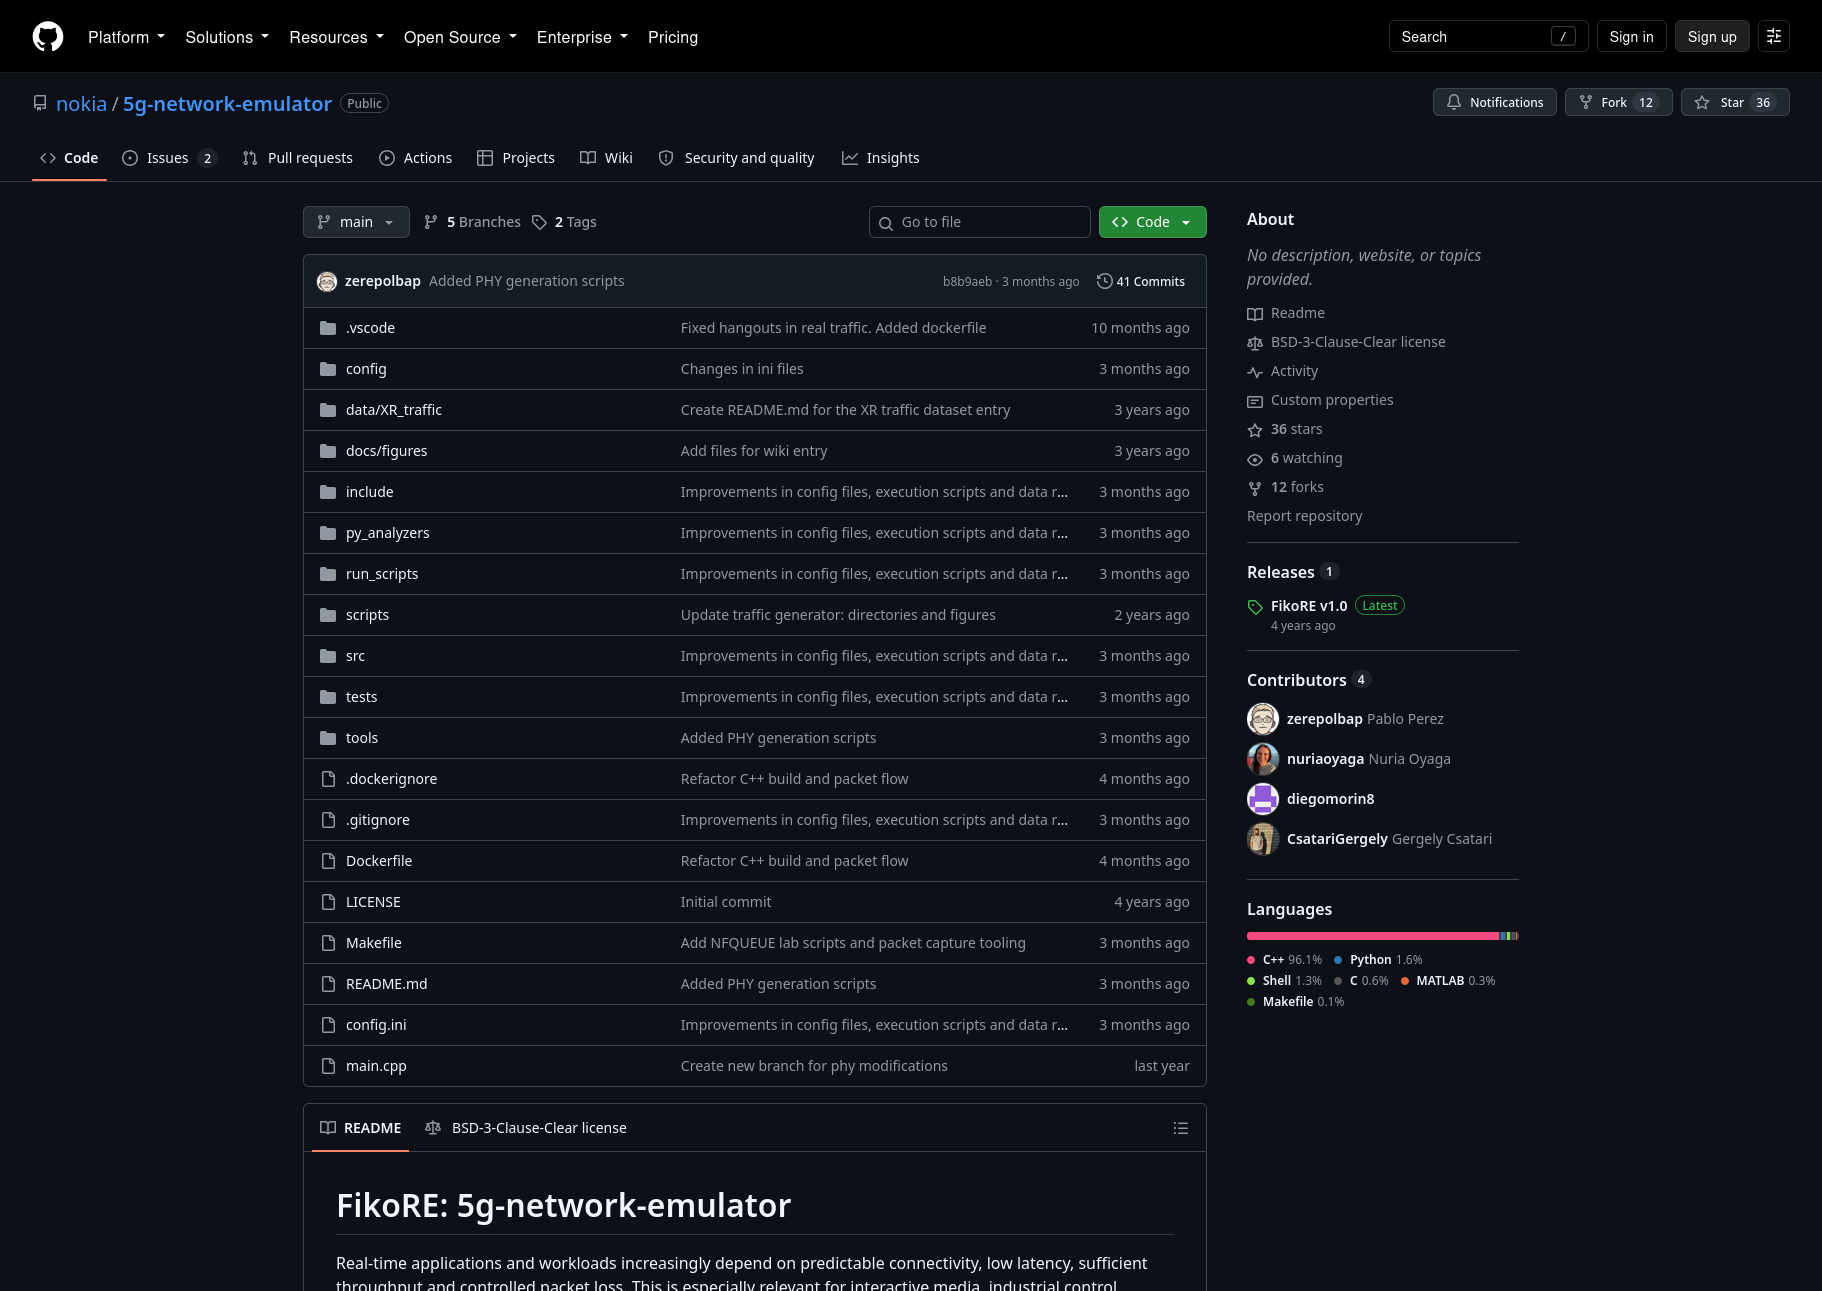
\includegraphics[height=2.5cm]{../memoria/imagenes/emuladores/Screenshot_2026-09-13_at_18-58-57_GitHub_-_nokia_5g-network-emulator___GitHub_cropped.png}

\vspace{1.0cm}


\includegraphics[height=0.5cm]{../memoria/imagenes/nokia/Nokia_2023.svg.png}

+


\includegraphics[height=1.0cm]{../memoria/imagenes/Logo_UC3M.svg.png}
\end{center}
\end{column}
\end{columns}
\end{frame}

% Diapositiva
\begin{frame}
\frametitle{Estado de la cuestión (III)}

\begin{itemize}
\item {
	Planificación de paquetes.
	\begin{itemize}
	\item Asignación de los recursos de radio.
	\item Literatura extensa.
	\item {
		Necesidad de validación.
		\begin{itemize}
		\item Despliegue real de 5G caros, poco flexible.
		\item Emulador barato, se puede reajustar para probar estrategias.
		\end{itemize}
	}
	\end{itemize}
}
\end{itemize}

\begin{center}
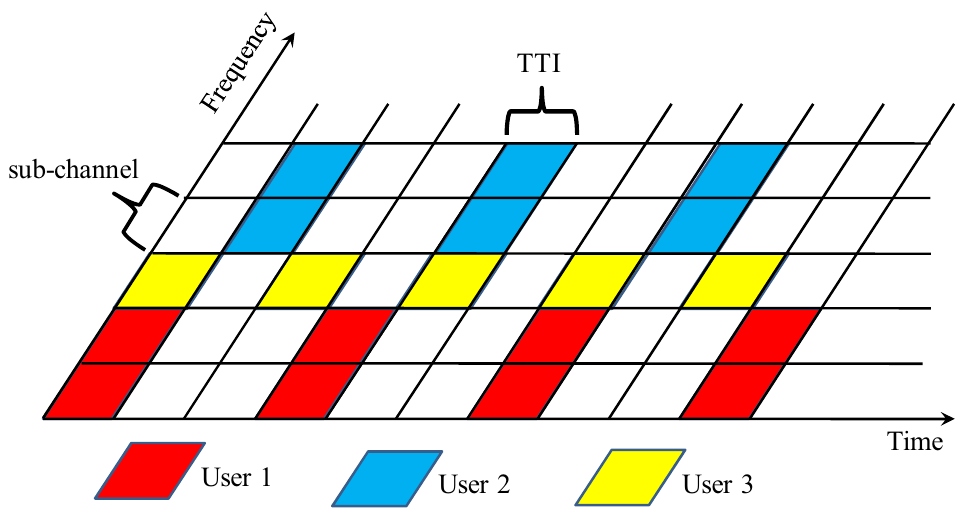
\includegraphics[height=4.0cm]{../memoria/imagenes/scheduling_italianos/scheduling_italianos-198.png}
\end{center}
\end{frame}

% Diapositiva
\begin{frame}
\frametitle{Estado de la cuestión (IV)}

\begin{itemize}
\item {
	Comunicaciones en entornos vehiculares (C-V2X).
	\begin{itemize}
	\item {
		Importancia.
		\begin{itemize}
		\item La automoción es de los sectores más impactados.
		\item La automoción es fundamental en la economía.
		\end{itemize}
	}
	\item {
		Desarrollo.
		\begin{itemize}
		\item Numerosas iniciativas de investigación.
		\item 3GPP ya incluyó C-V2X entre sus prioridades.
		\item \textit{FikoRE} puede representar escenarios de C-V2X.
		\end{itemize}
	}
	\end{itemize}
}
\end{itemize}

\begin{center}
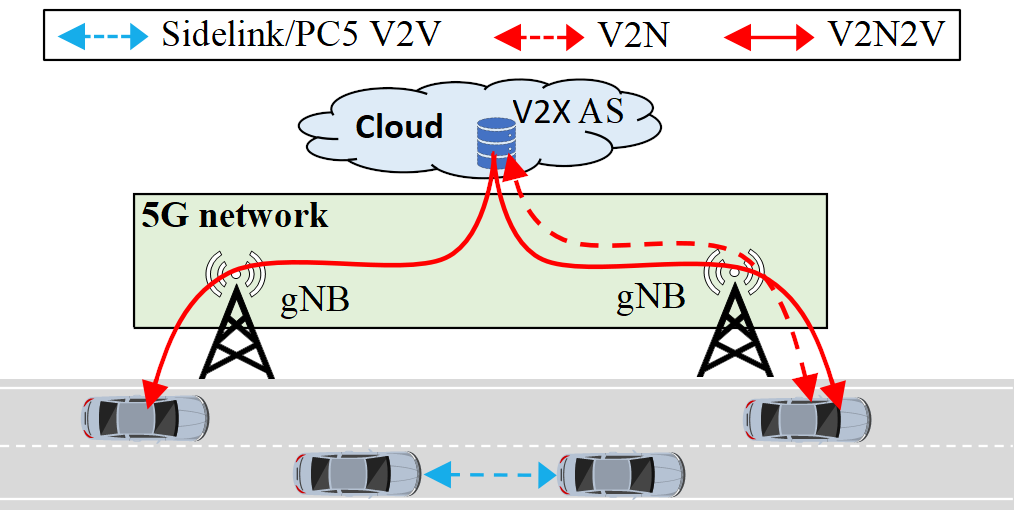
\includegraphics[height=3.0cm]{../memoria/imagenes/v2x_umh/v2x_umh-000.png}
\end{center}
\end{frame}

% Diapositiva
\begin{frame}
\frametitle{Estado de la cuestión (V)}

\begin{itemize}
\item {
	Otros casos de uso.
	\begin{itemize}
	\item Servicio URLLC. $\rightarrow$ Comunicaciones fiables y de muy baja latencia. $\rightarrow$ Aplicaciones que dependen de la seguridad.
	\item AR/VR/MR. $\rightarrow$ Dependen por completo de 5G.
	\item Se pueden recrear con \textit{FikoRE}.
	\end{itemize}
}
\end{itemize}

\begin{center}
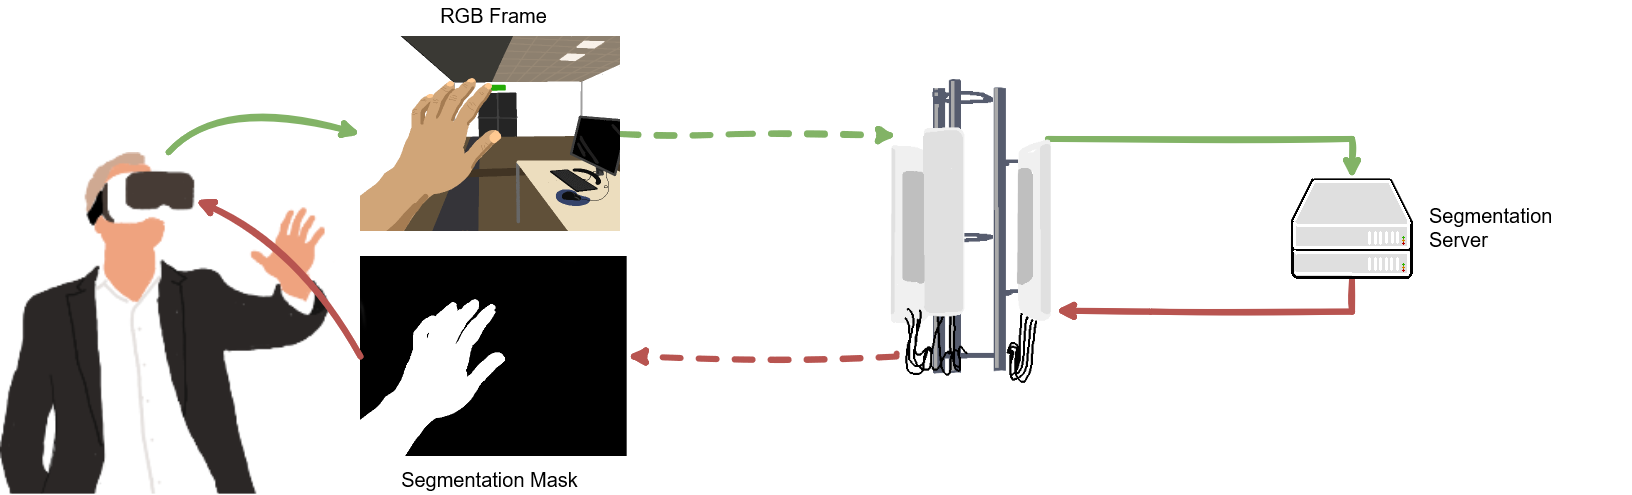
\includegraphics[height=3.5cm]{../memoria/imagenes/fikore_doc/figures/XROffloadingExample.png}
\end{center}
\end{frame}

% SUBSECCIÓN
\subsection{Estructura del trabajo}

% Diapositiva
\begin{frame}
\frametitle{Estructura del trabajo (I)}

\begin{itemize}
\item Objetivo. $\rightarrow$ Evaluar despliegues de 5G y de aplicaciones para 5G mediante el emulador \textit{FikoRE}.
\item {
	Sección ``Interfaz de radio de 5G''.
	\begin{itemize}
	\item Descripción de la interfaz de radio de 5G.
	\item Conceptos de redes móviles.
	\item Simulación y emulación de la interfaz de radio.
	\end{itemize}
}
\item {
	Sección ``Emulador \textit{FikoRE}''.
	\begin{itemize}
	\item Características más importantes.
	\item Procedimientos para emular la interfaz de radio.
	\item Capacidades de emulación.
	\end{itemize}
}
\end{itemize}
\end{frame}

% Diapositiva
\begin{frame}
\frametitle{Estructura del trabajo (II)}

\begin{itemize}
\item {
	Sección ``Caso de uso: planificación de paquetes (\textit{packet scheduling})''.
	\begin{itemize}
	\item Estudio y diseño de planificación de paquetes.
	\item Varias simulaciones.
	\item Conclusiones sobre el diseño del planificador de paquetes.
	\end{itemize}
}
\item {
	Sección ``Caso de uso: comunicaciones celulares en entornos vehiculares (C-V2X)''.
	\begin{itemize}
	\item Estudio y diseño para C-V2X.
	\item Varias simulaciones.
	\item Conclusiones sobre el diseño para C-V2X y sobre su viabilidad.
	\end{itemize}
}
\item {
	Sección ``Conclusiones''.
	\begin{itemize}
	\item Se recopilan las conclusiones del trabajo.
	\end{itemize}
}
\end{itemize}
\end{frame}





% SECCIÓN
\section{Interfaz de radio de 5G}

% Diapositiva
\begin{frame}
\frametitle{Qué es la interfaz de radio}

\begin{itemize}
\item Parte de la RAN que que se ocupa de la transmisión entre la BS y el UE.
\item Interfaz de radio $\neq$ Red de acceso
\item Interfaz de radio $\neq$ Capa física
\item Sistemas de comunicaciones $\rightarrow$ Redes móviles $\rightarrow$ Sistema 5G $\rightarrow$ RAN $\rightarrow$ Interfaz de radio
\end{itemize}
\end{frame}

% SUBSECCIÓN
\subsection{Fundamentos de comunicaciones móviles}

% Diapositiva
\begin{frame}
\frametitle{Fundamentos - Arquitectura - Básico}

\begin{itemize}
\item {
	Sistema de comunicaciones móviles (PLMN, PMR) $\rightarrow$ Arquitectura convencional:
	\begin{itemize}
	\item Red de acceso (RAN): Elementos de red que permiten al usuario acceder a servicios de comunicaciones.
	\item {
		Red de tránsito: Elementos de red que interconectan redes de acceso distintas.
		\begin{itemize}
		\item Núcleo de red (\textit{Core Network}): Realiza funciones de conmutación de circuitos y paquetes.
		\item \textit{backhaul}: Elementos intermedios para conectar la red de acceso con el núcleo de red.
		\end{itemize}
	}
	\end{itemize}
}
\item {
	Una tecnología de PLMN $\rightarrow$ Una arquitectura distintiva:
	\begin{itemize}
	\item Descripción funcional: Los distintos elementos o entidades funcionales que componen la red, incluyendo la RAN.
	\item Protocolos e interfaces de red: Los medios de comunicación entre elementos y los métodos de funcionamiento.
	\end{itemize}
}
\end{itemize}
\end{frame}

% Diapositiva
\begin{frame}
\frametitle{Fundamentos - Arquitectura - Descripción funcional}

\begin{itemize}
\item {
	RAN:
	\begin{itemize}
	\item Terminal de usuario (\textit{User Equipment}, UE): Es la máquina que usa el usuario para conectarse a la red.
	\item Estación base (\textit{Base Station}, BS): Es la máquina a la que se conecta el UE.
	\end{itemize}
}
\item {
	\textit{Core Network}:
	\begin{itemize}
	\item Funciones del plano de control (registro, autentificación, seguimiento y aviso a los UE).
	\item Nodo de conmutación de paquetes, funciones del plano de usuario.
	\item Conexión del núcleo de red con redes externas.
	\end{itemize}
}
\end{itemize}

\begin{center}
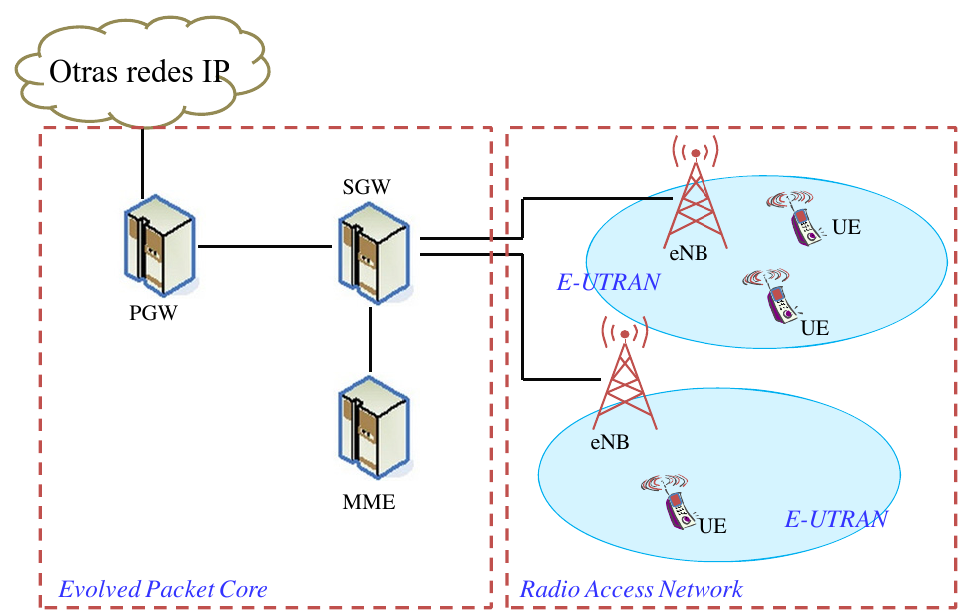
\includegraphics[height=3.5cm]{../memoria/imagenes/scheduling_italianos/scheduling_italianos-001_es.png}
\end{center}
\end{frame}

% Diapositiva
\begin{frame}
\frametitle{Fundamentos - Arquitectura - Protocolos e interfaces (I)}

\begin{itemize}
\item {
	Interfaces.
	\begin{itemize}
	\item Medio de por el que se conectan dos entidades y su protocolo de funcionamiento.
	\end{itemize}

	\begin{center}
	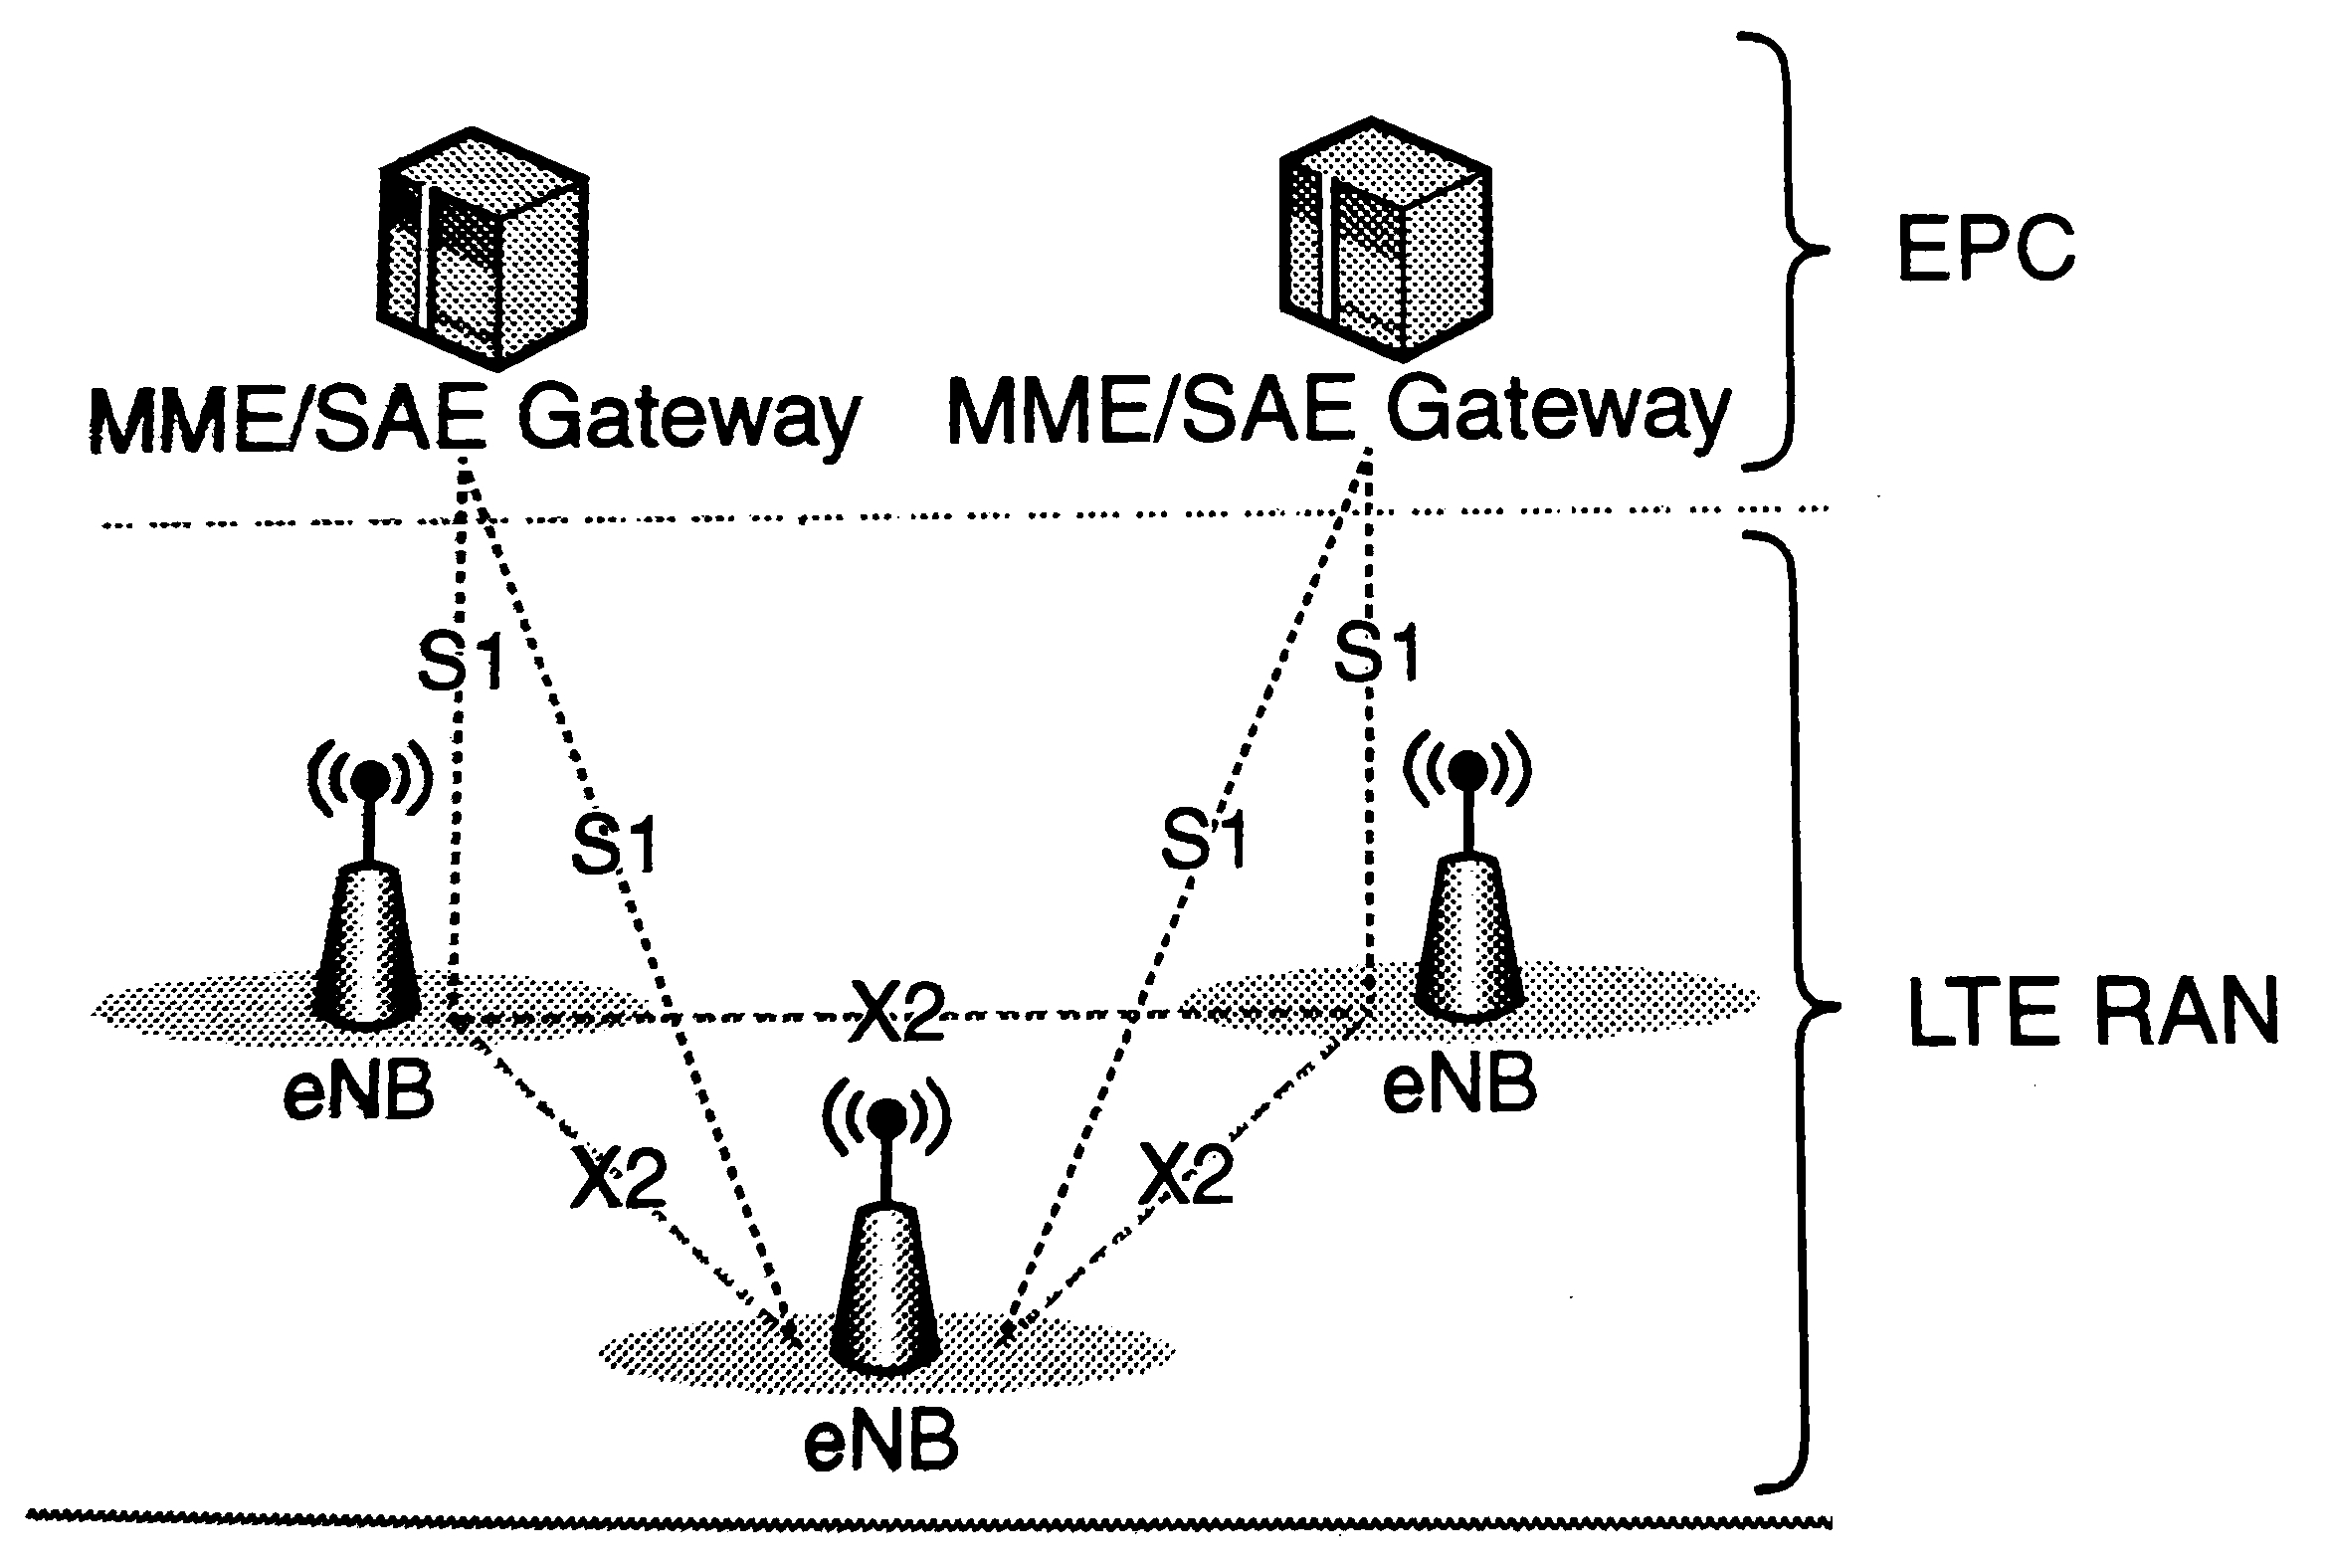
\includegraphics[height=4.5cm]{../memoria/imagenes/comunicaciones_moviles/cm_cap10_1_fixed.jpg}
	\end{center}
}
\end{itemize}
\end{frame}

% % Diapositiva
% \begin{frame}
% \frametitle{Fundamentos - Arquitectura - Protocolos e interfaces (II)}
%
% \begin{itemize}
% \item {
% 	Protocolos.
% 	\begin{itemize}
% 	\item Permiten interactuar entre los elementos de la red de manera ordenada e implementar las funciones de la red.
% 	\item {
% 		Usan \textit{canales}:
% 		\begin{itemize}
% 		\item Canales lógicos.
% 		\item Canales de transporte.
% 		\item Canales de físicos.
% 		\end{itemize}
% 	}
% 	\item Usan \textit{señales}.
% 	\end{itemize}
%
% 	\begin{center}
% 	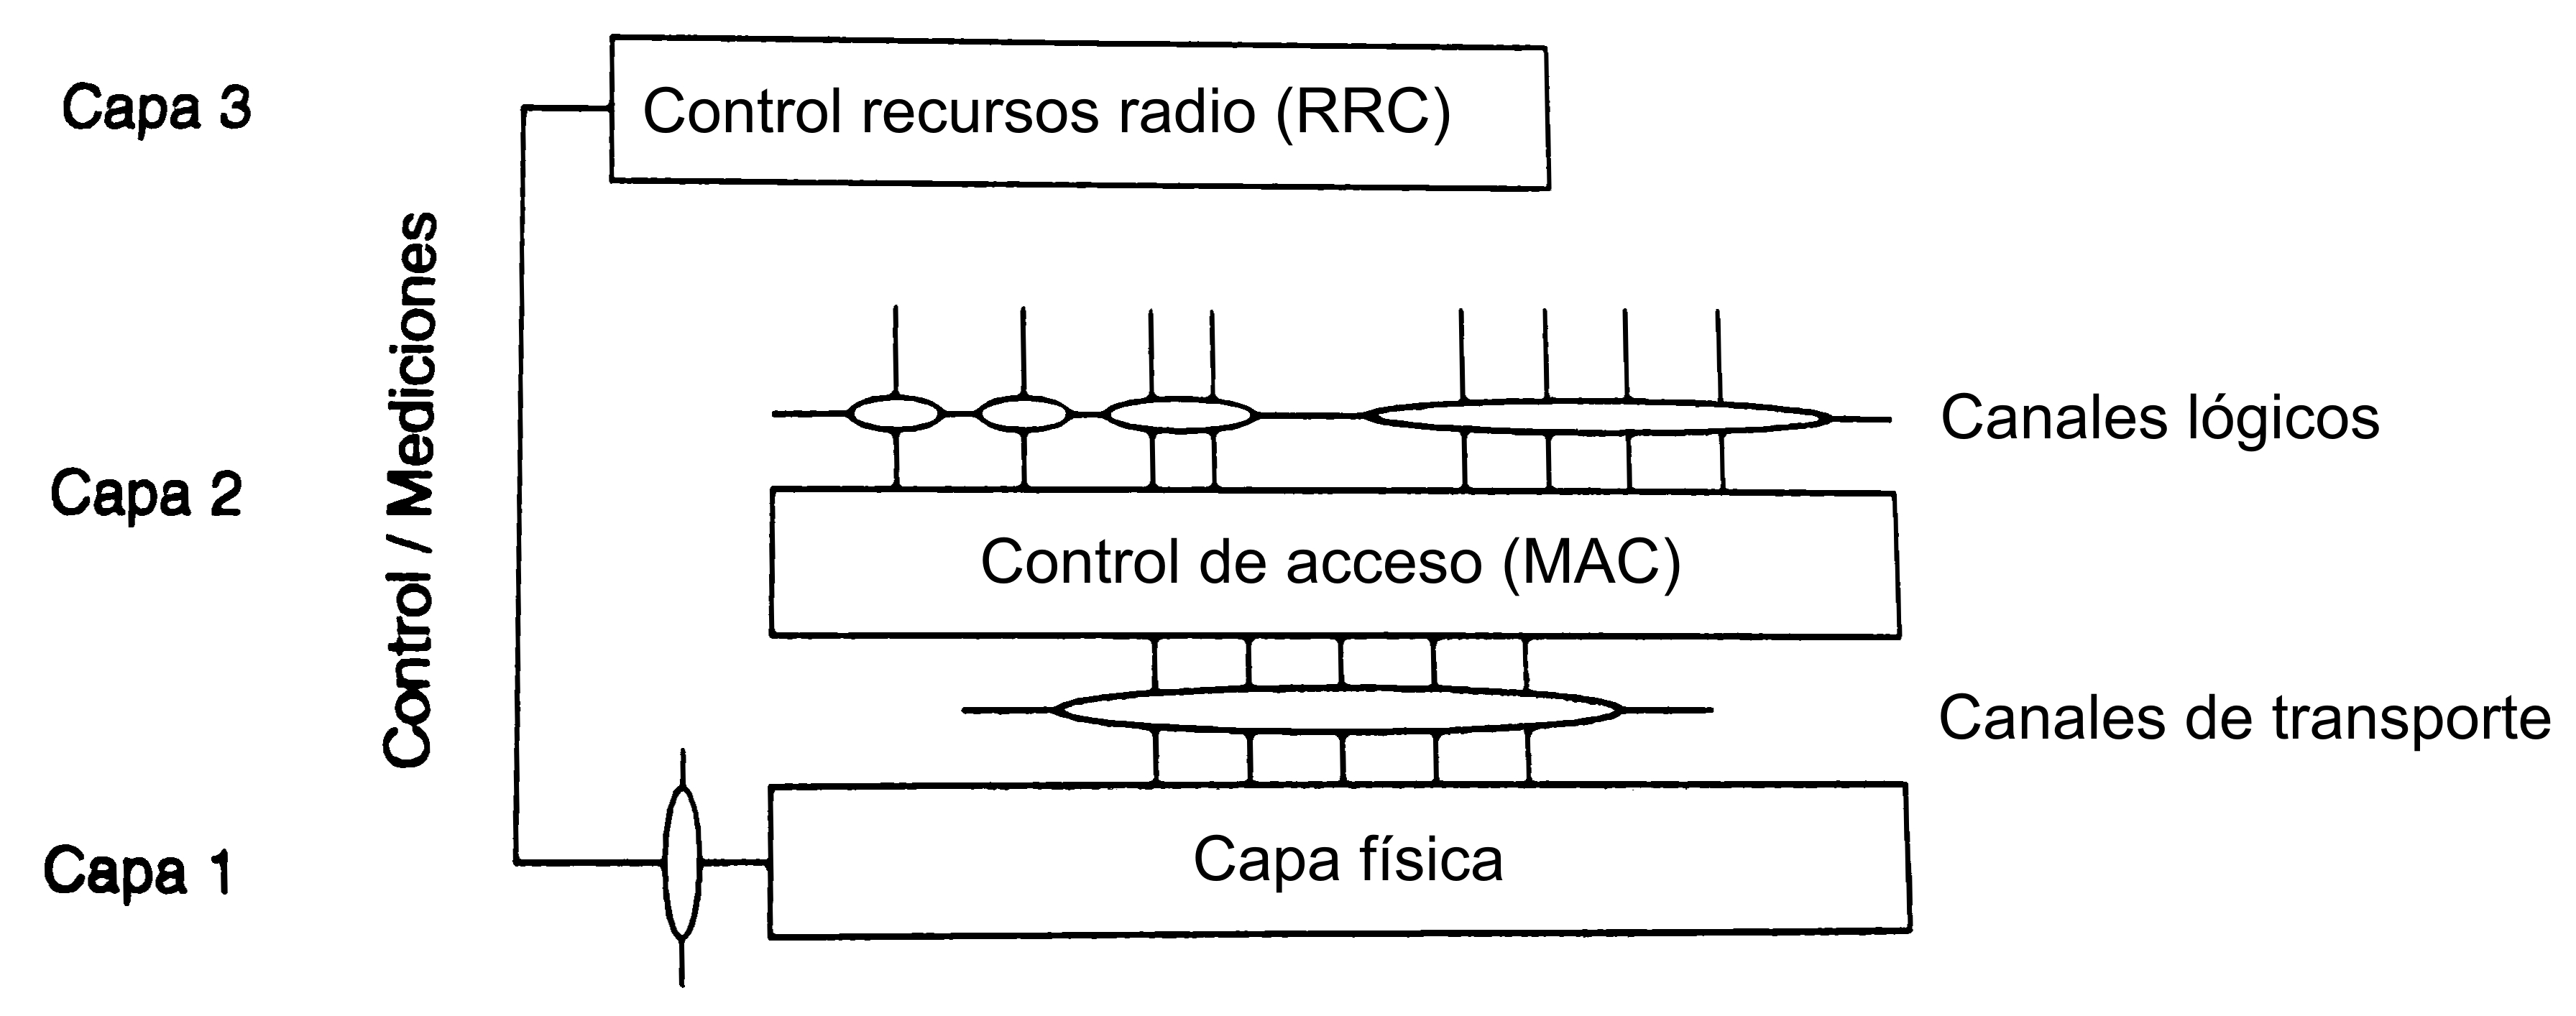
\includegraphics[height=3.5cm]{../memoria/imagenes/comunicaciones_moviles/cm_cap10_2_fixed.jpg}
%
% 	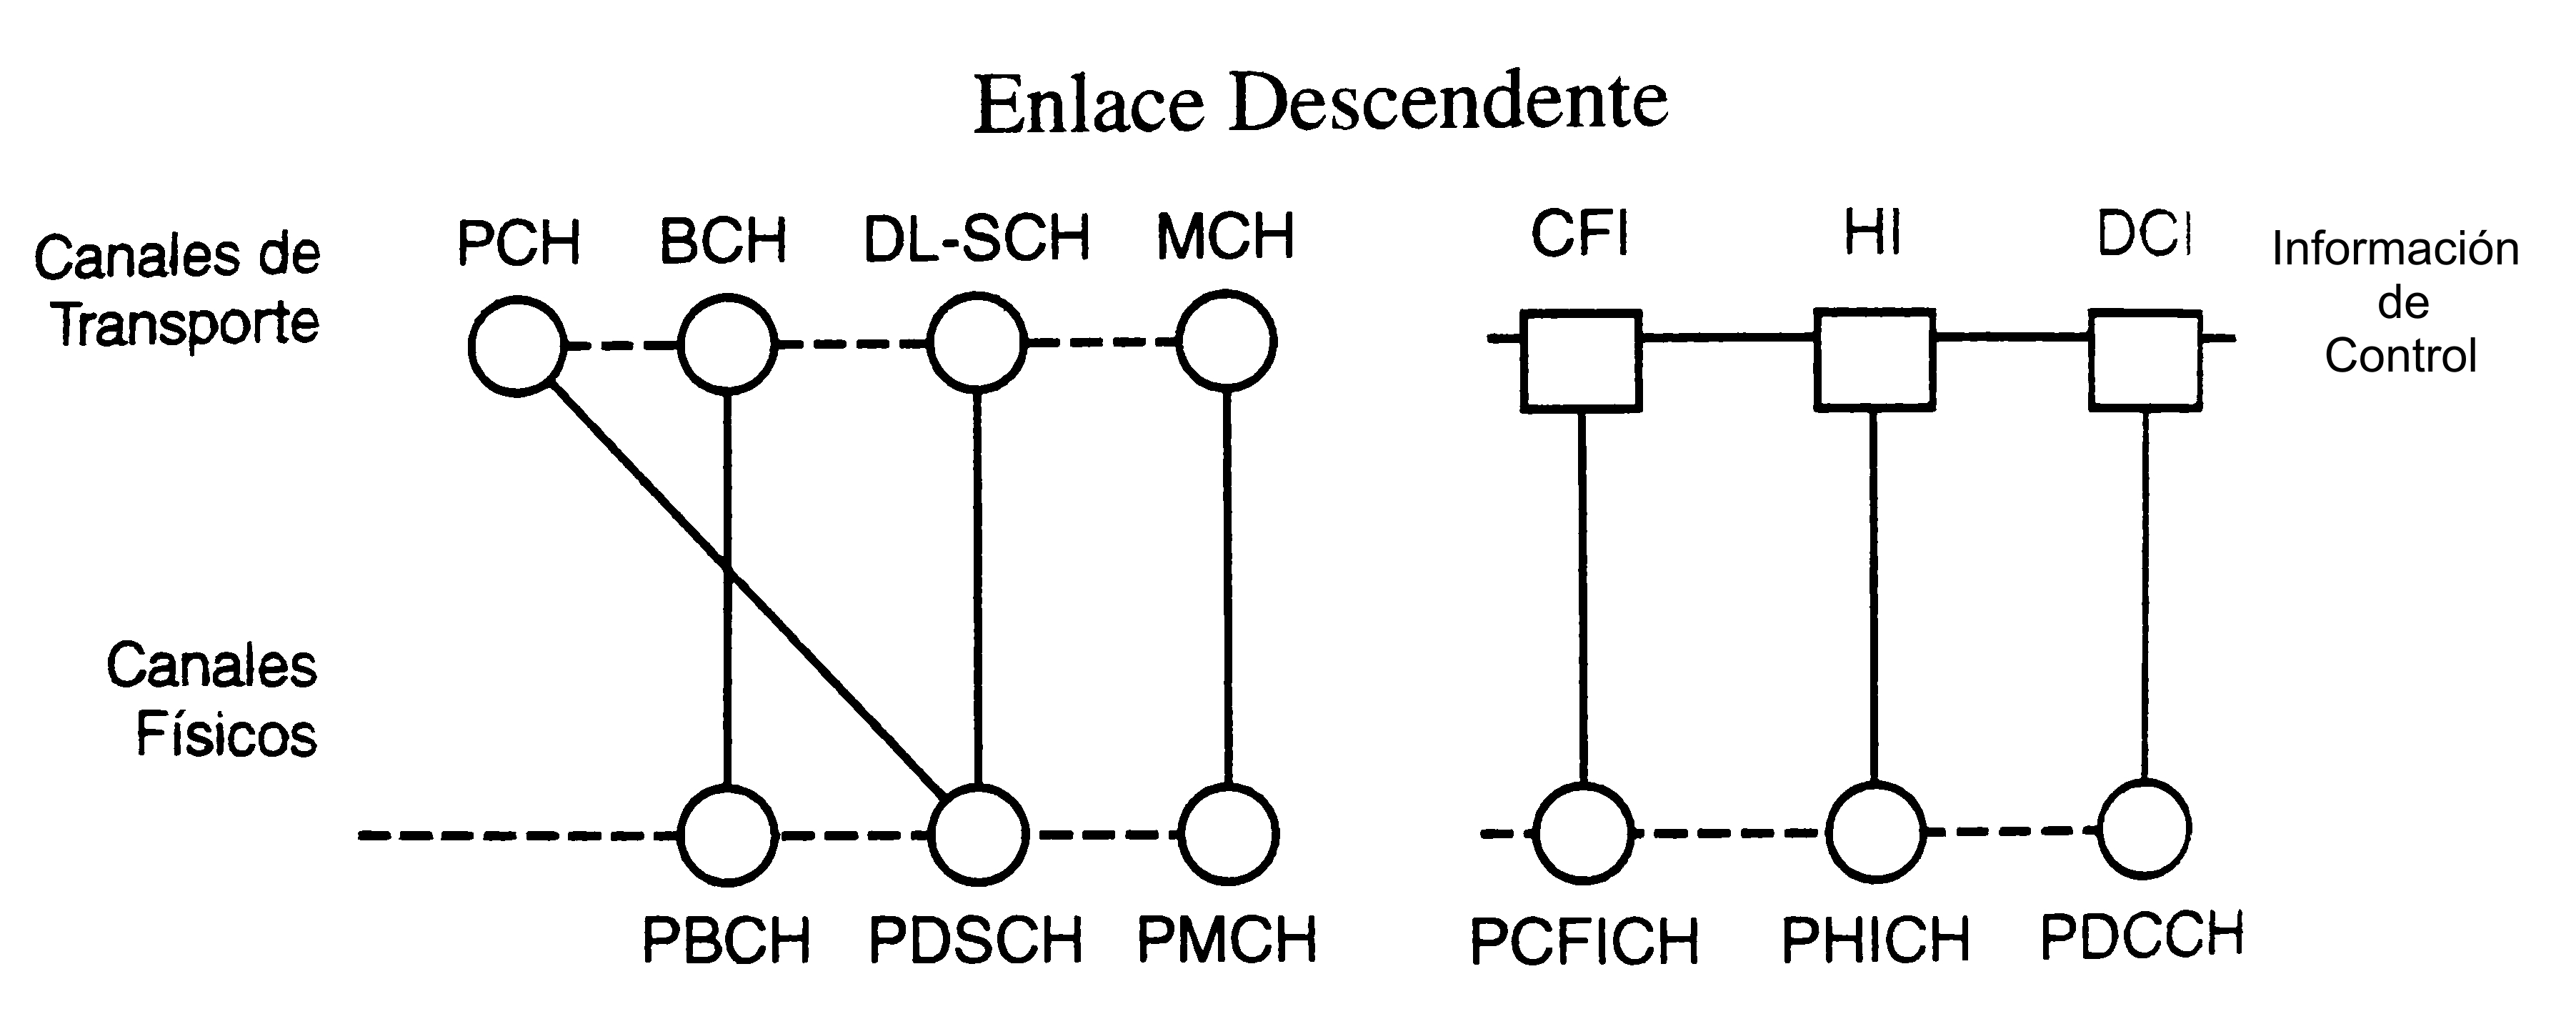
\includegraphics[height=3.5cm]{../memoria/imagenes/comunicaciones_moviles/cm_cap10_3_fixed.jpg}
%
% 	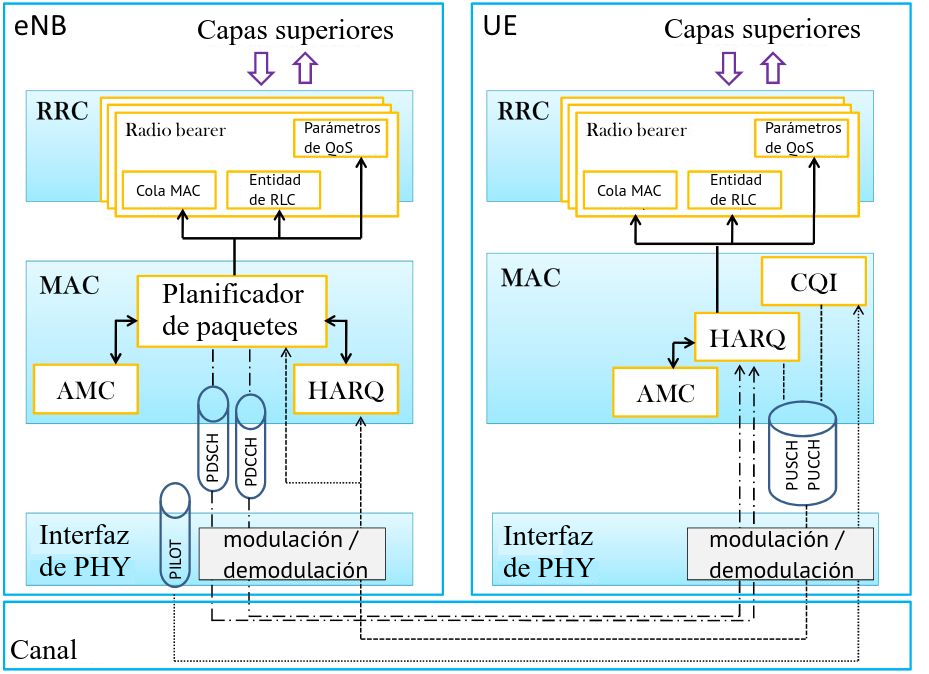
\includegraphics[height=3.5cm]{../memoria/imagenes/scheduling_italianos/scheduling_italianos-172_es.png}
% 	\end{center}
% }
% \end{itemize}
% \end{frame}

% Diapositiva
\begin{frame}
\frametitle{Fundamentos - Arquitectura - Protocolos e interfaces (II)}

\begin{itemize}
\item {
	Protocolos.
	\begin{itemize}
	\item Permiten interactuar entre los elementos de la red de manera ordenada e implementar las funciones de la red.
	\item {
		Usan \textit{canales}:
		\begin{itemize}
		\item Canales lógicos.
		\item Canales de transporte.
		\item Canales de físicos.
		\end{itemize}
	}
	\item Usan \textit{señales}.
	\end{itemize}

	\begin{center}
	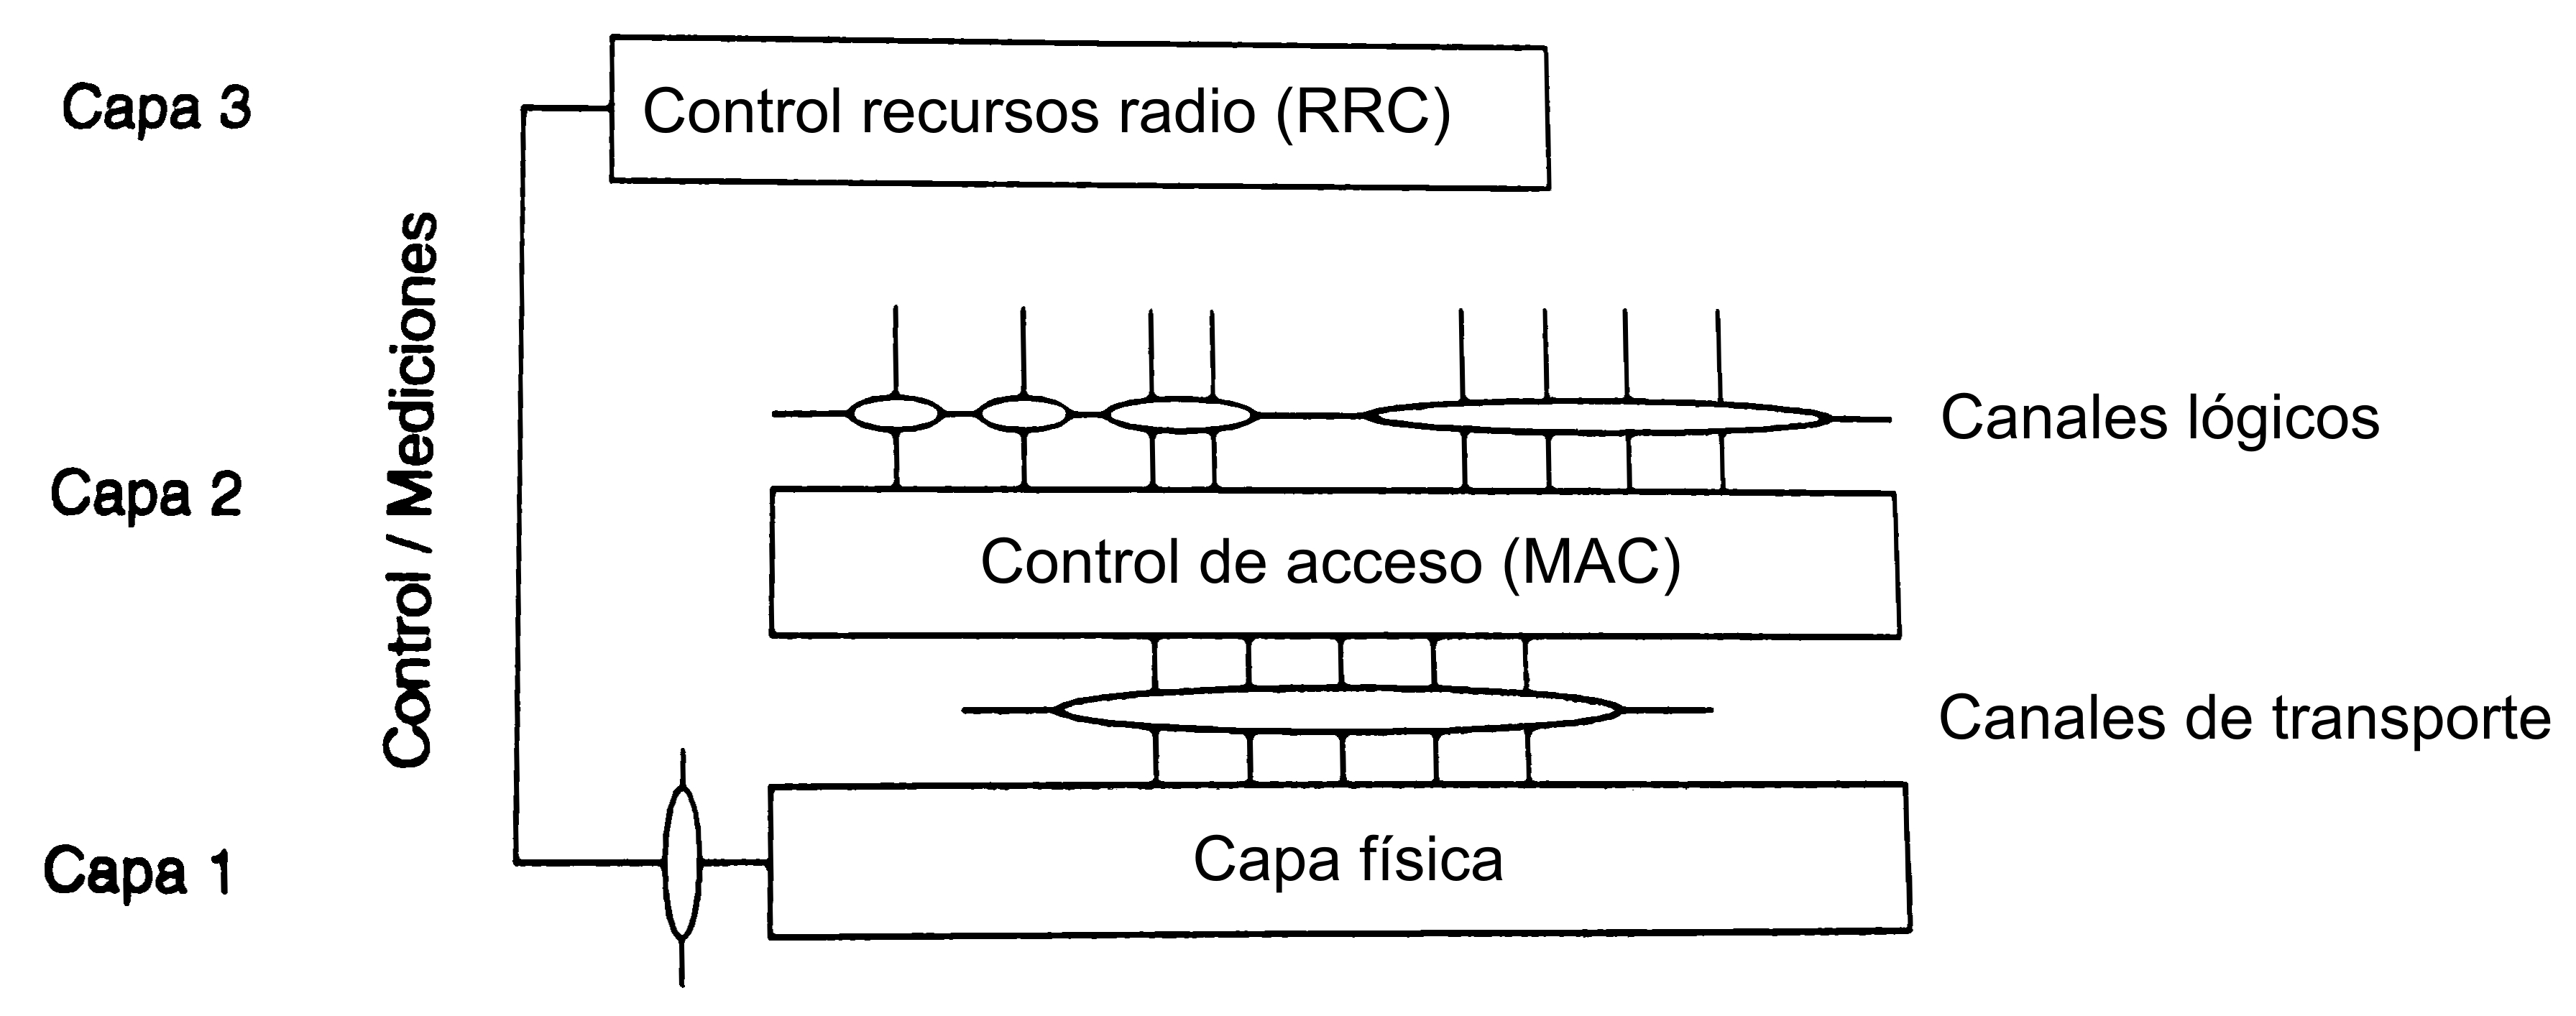
\includegraphics[height=3.5cm]{../memoria/imagenes/comunicaciones_moviles/cm_cap10_2_fixed.jpg}
	\end{center}
}
\end{itemize}
\end{frame}

% Diapositiva
\begin{frame}
\frametitle{Fundamentos - Arquitectura - Protocolos e interfaces (III)}

\begin{center}
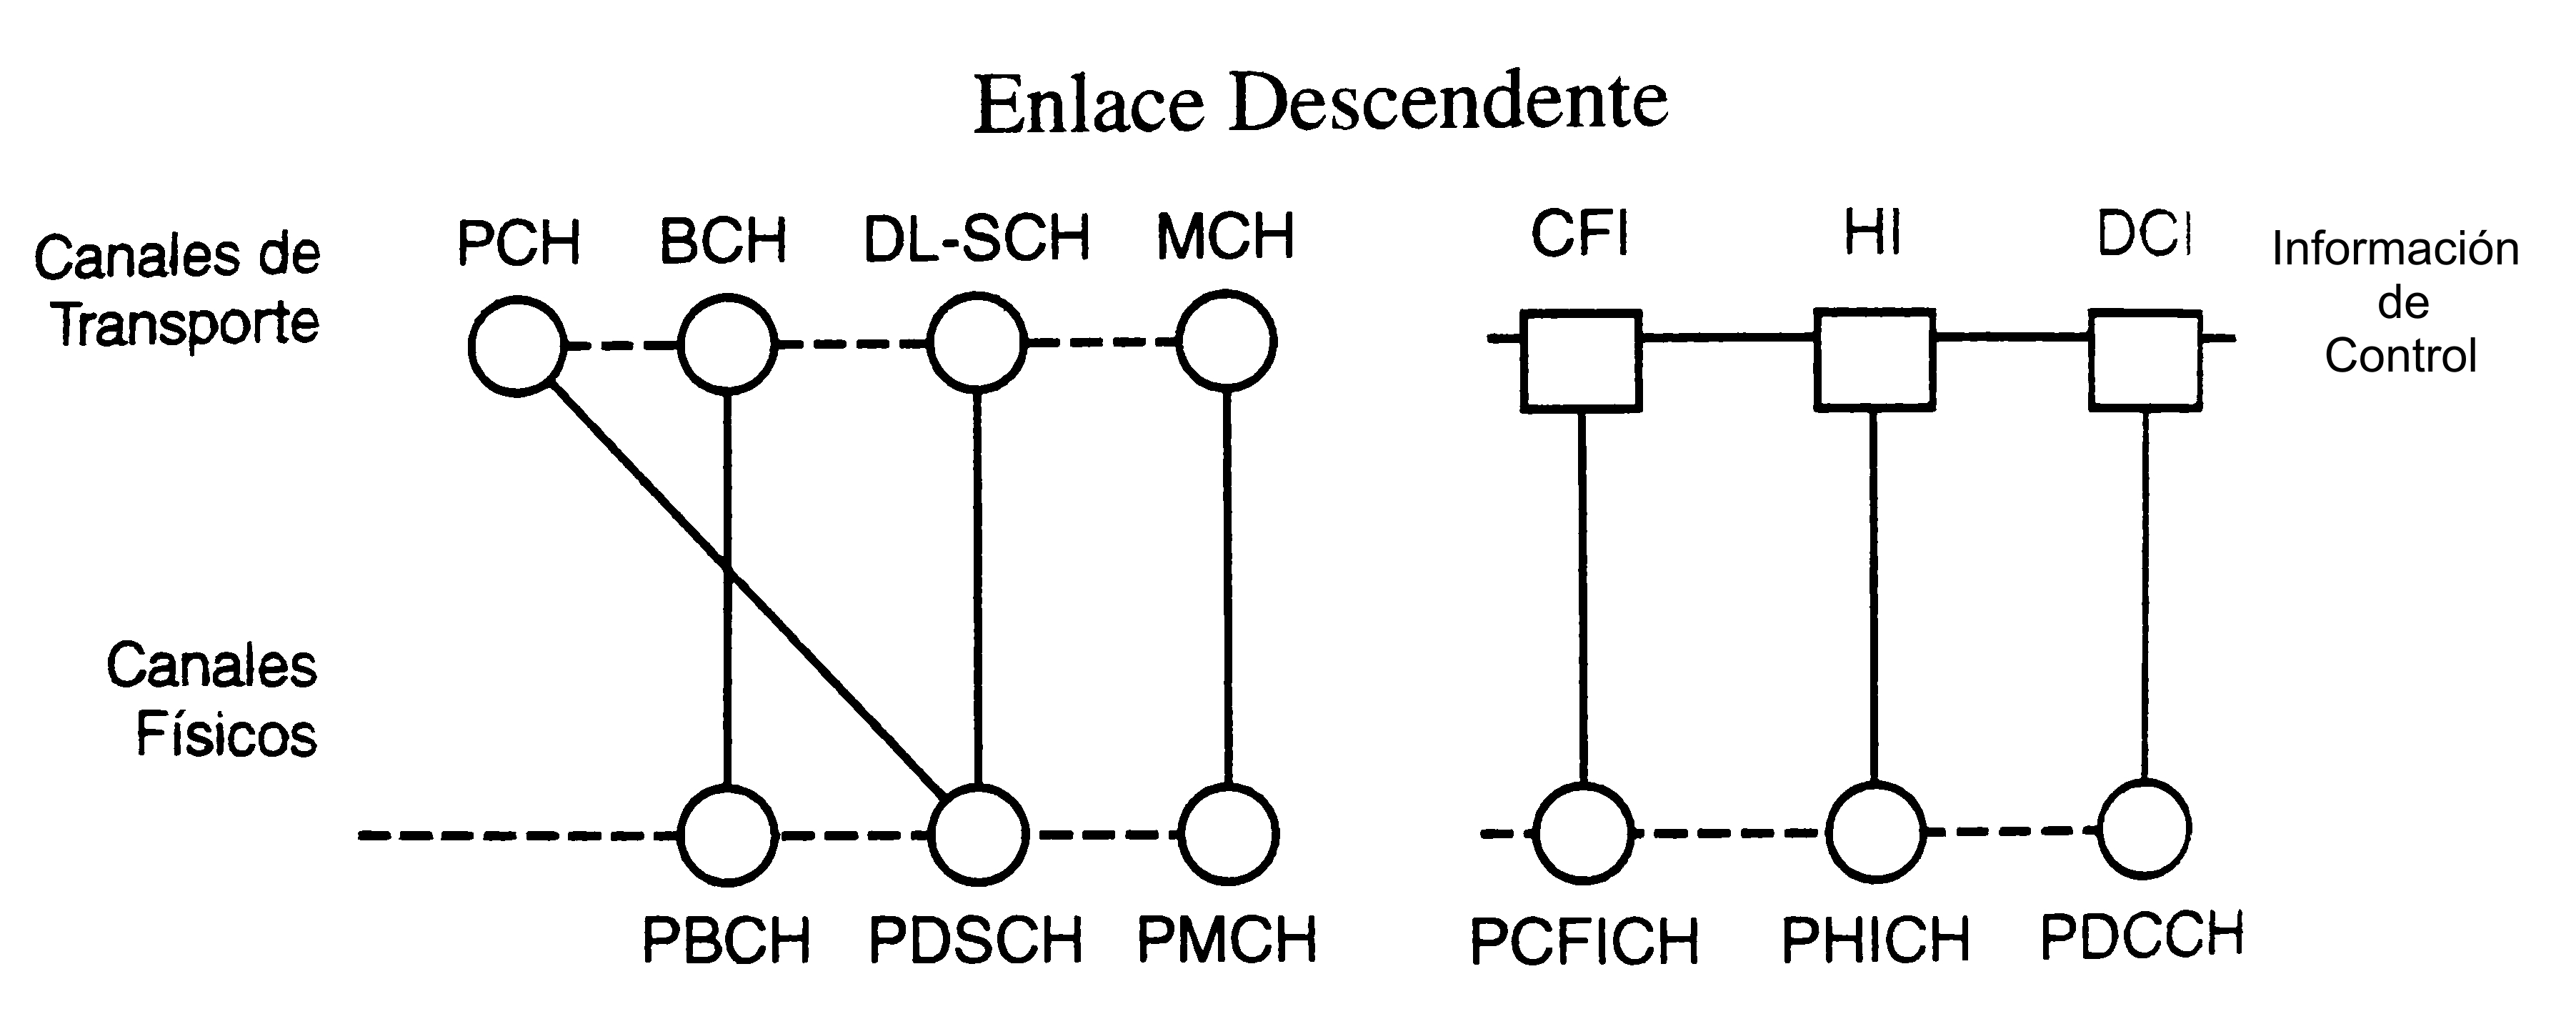
\includegraphics[height=3.5cm]{../memoria/imagenes/comunicaciones_moviles/cm_cap10_3_fixed.jpg}
\end{center}
\end{frame}

% Diapositiva
\begin{frame}
\frametitle{Fundamentos - Arquitectura - Protocolos e interfaces (IV)}

\begin{center}
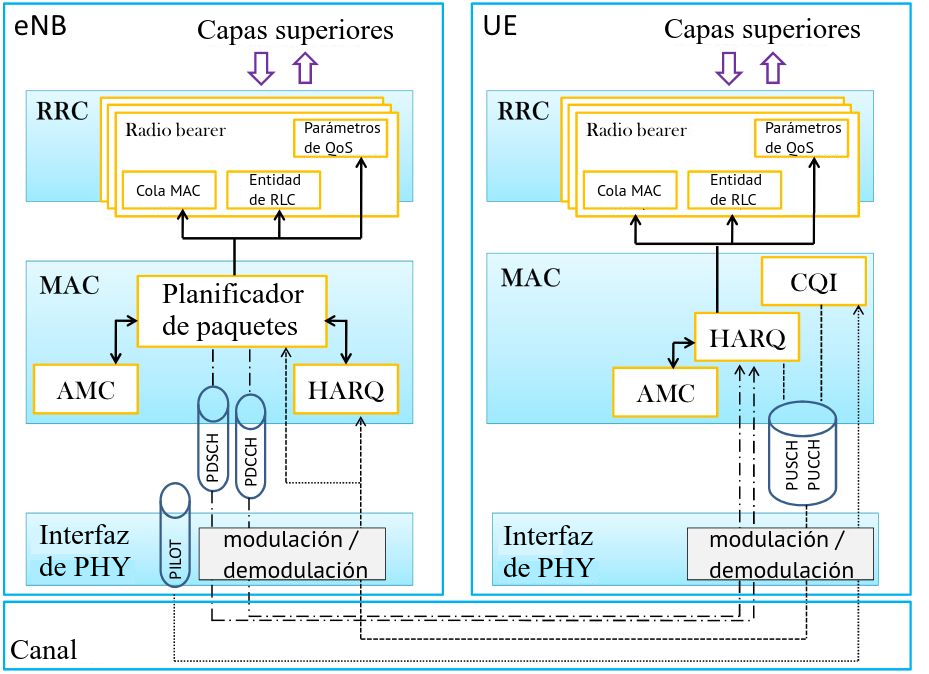
\includegraphics[height=7.0cm]{../memoria/imagenes/scheduling_italianos/scheduling_italianos-172_es.png}
\end{center}
\end{frame}

% % Diapositiva
% \begin{frame}
% \frametitle{Fundamentos - Transmisión inalámbrica - Transmisión en el enlace radioeléctrico}
%
% \begin{itemize}
% \item Ruido:
% $$P_{rx} = P_{tx} + P_{N}$$
% Relación portadora a ruido:
% $$\frac{C}{N}$$
% Relación de protección:
% $$\frac{C}{N} = \frac{P_{tx}}{P_{N}} \rightarrow \left( \frac{C}{N} \right)_{dB} = 10 \log P_{tx} - 10 \log P_{N} > R_p$$
% \item Interferencia:
% $$P_{rx} = P_{tx} + P_{I}$$
% Relación portadora a interferencia:
% $$\frac{C}{I}$$
% Relación de protección:
% $$\frac{C}{I} = \frac{P_{tx}}{P_{I}} \rightarrow \left( \frac{C}{I} \right)_{dB} = 10 \log P_{tx} - 10 \log P_{I} > R_p$$
% \item Pérdida por propagación (atenuación):
% $$l_b = l_{att} (d) = k \cdot d^n \rightarrow L_b = L_{att} (d) = 10 \log (k) +10 n \log (d)$$
% \item Desvanecimiento por sombra (\textit{shadow fading}):
% $$L_b = L_{att} (d) + L_{sf} (x, y)$$
% $$L_{sf} (x, y) \sim \operatorname{\mathcal{N}} (\mu, \sigma)$$
% \item Desvanecimiento por multitrayecto (\textit{multipath fading}):
% $$L_b = L_{att} (d) + L_{sf} (x, y) + L_{ff} (t, f) $$
% $$\operatorname{P} \left( L_{ff} (t, f) = r \right) = \frac{r}{b} \exp \left( \frac{-r^2}{2 b} \right), b = \frac{\bar{r^2}}{2}$$
%
% \begin{center}
% 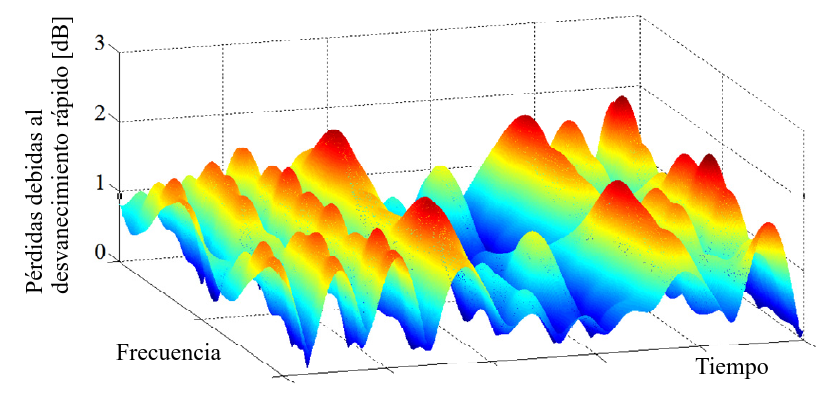
\includegraphics[height=3.5cm]{../memoria/imagenes/scheduling_italianos/scheduling_italianos-174_es.png}
% \end{center}
% \end{itemize}
%
% \begin{center}
% 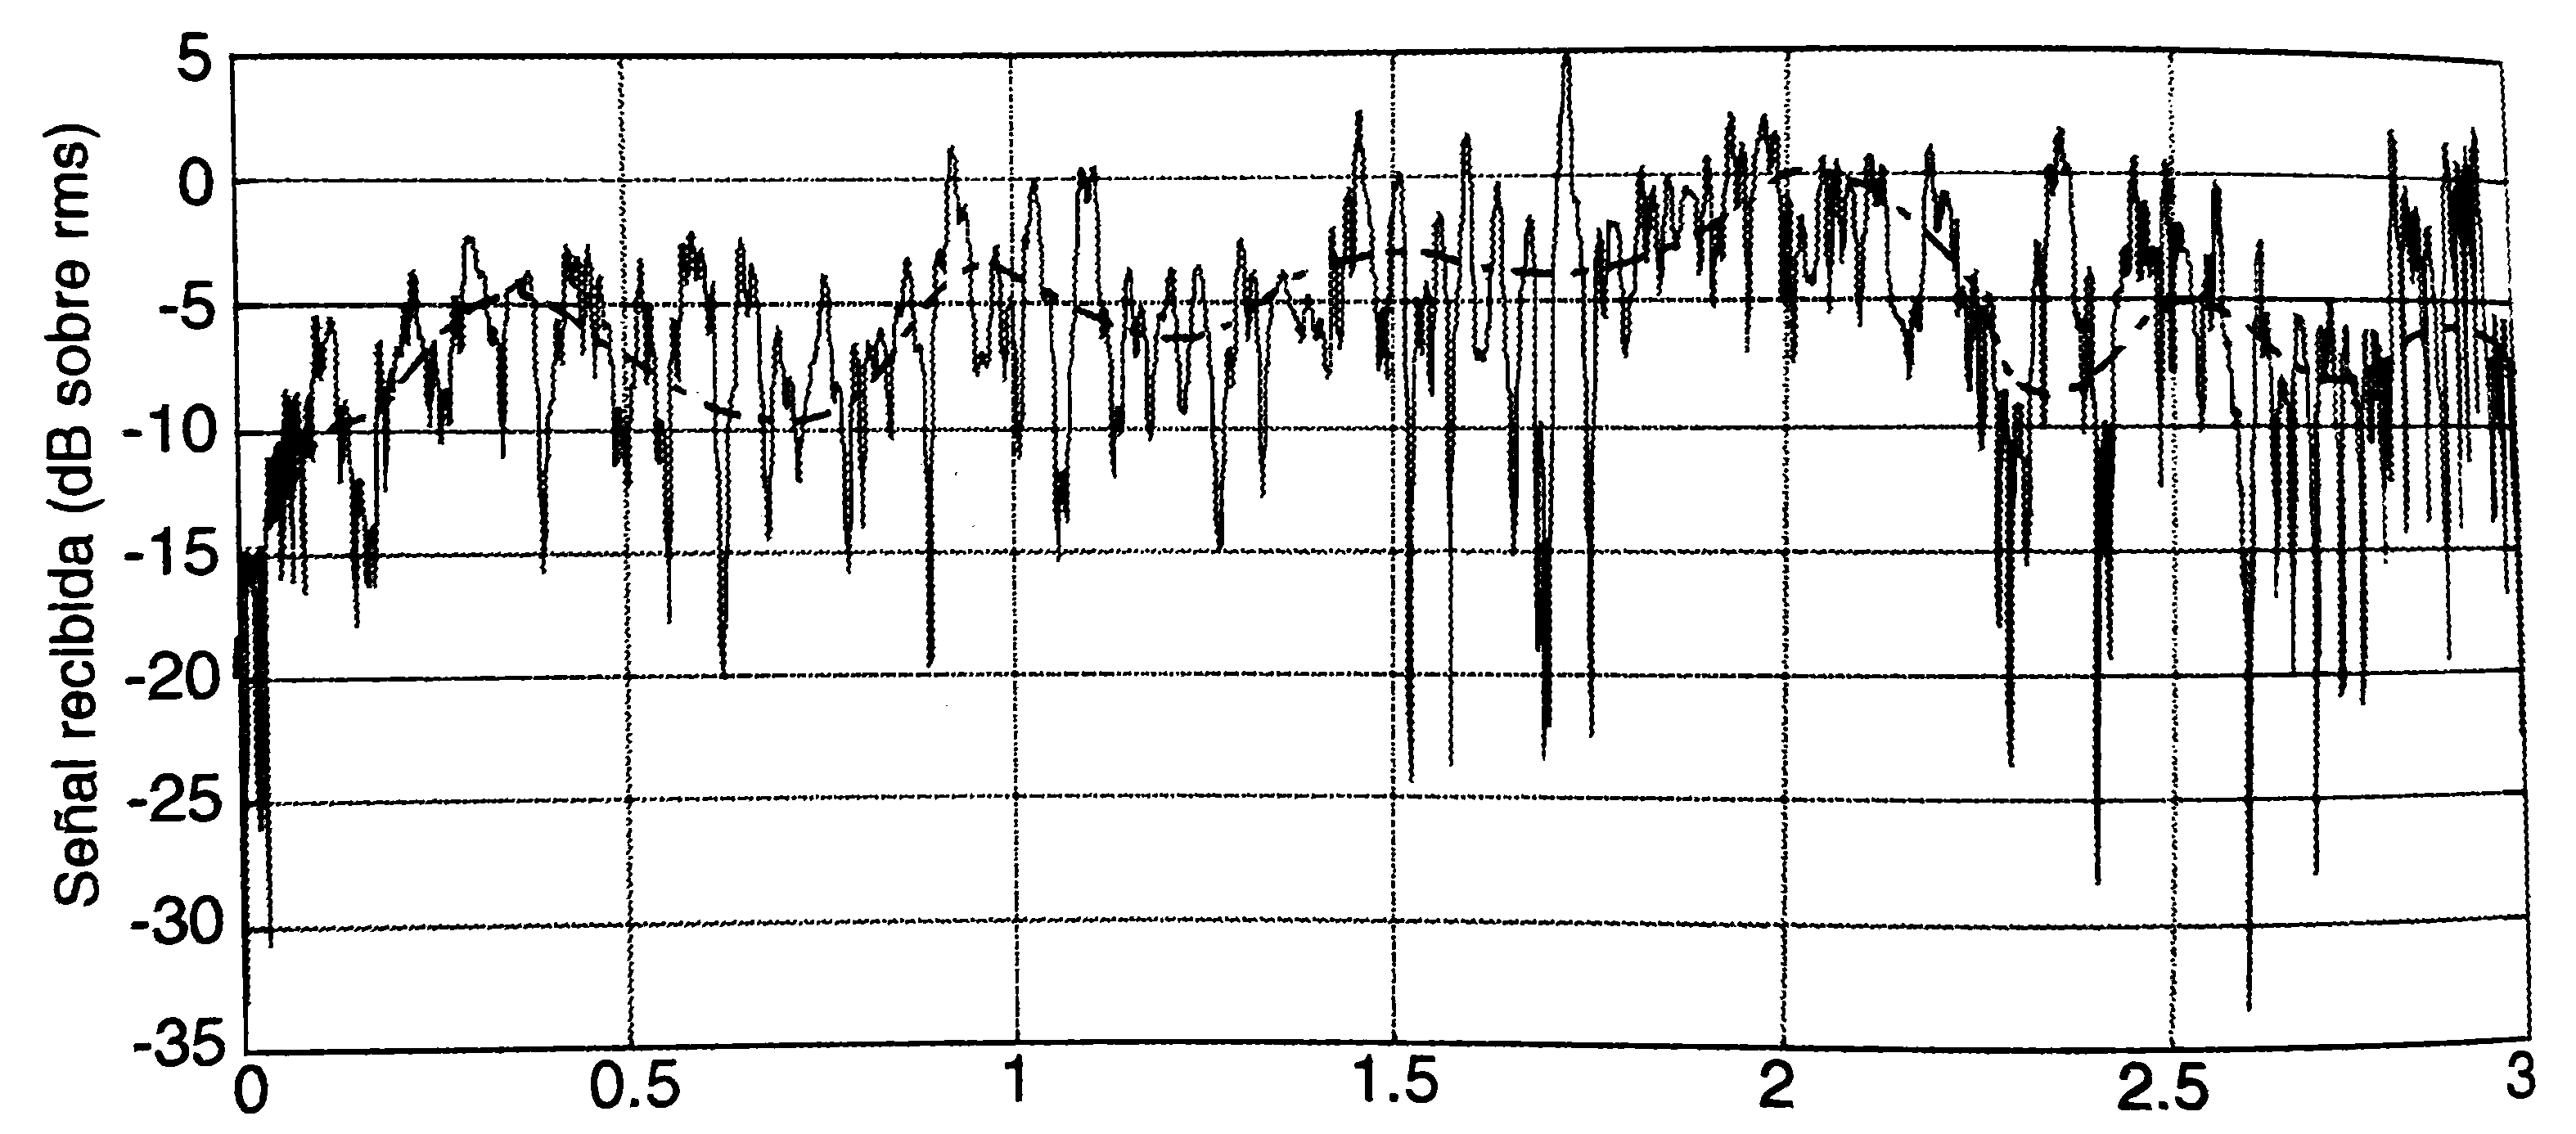
\includegraphics[height=5.0cm]{../memoria/imagenes/comunicaciones_moviles/cm_cap3_2_fixed.jpg}
% \end{center}
% \end{frame}

% Diapositiva
\begin{frame}
\frametitle{Fundamentos - Transmisión inalámbrica - Transmisión en el enlace radioeléctrico (I)}

\begin{itemize}
\item Ruido:
$$P_{rx} = P_{tx} + P_{N}$$
Relación portadora a ruido:
$$\frac{C}{N}$$
Relación de protección:
$$\frac{C}{N} = \frac{P_{tx}}{P_{N}} \rightarrow \left( \frac{C}{N} \right)_{dB} = 10 \log P_{tx} - 10 \log P_{N} > R_p$$
\end{itemize}
\end{frame}

% Diapositiva
\begin{frame}
\frametitle{Fundamentos - Transmisión inalámbrica - Transmisión en el enlace radioeléctrico (II)}

\begin{itemize}
\item Interferencia:
$$P_{rx} = P_{tx} + P_{I}$$
Relación portadora a interferencia:
$$\frac{C}{I}$$
Relación de protección:
$$\frac{C}{I} = \frac{P_{tx}}{P_{I}} \rightarrow \left( \frac{C}{I} \right)_{dB} = 10 \log P_{tx} - 10 \log P_{I} > R_p$$
\end{itemize}
\end{frame}

% Diapositiva
\begin{frame}
\frametitle{Fundamentos - Transmisión inalámbrica - Transmisión en el enlace radioeléctrico (III)}

\begin{itemize}
\item Pérdida por propagación (atenuación):
$$l_b = l_{att} (d) = k \cdot d^n \rightarrow L_b = L_{att} (d) = 10 \log (k) +10 n \log (d)$$
\item Desvanecimiento por sombra (\textit{shadow fading}):
$$L_b = L_{att} (d) + L_{sf} (x, y)$$
$$L_{sf} (x, y) \sim \operatorname{\mathcal{N}} (\mu, \sigma)$$
\end{itemize}
\end{frame}

% Diapositiva
\begin{frame}
\frametitle{Fundamentos - Transmisión inalámbrica - Transmisión en el enlace radioeléctrico (IV)}

\begin{itemize}
\item Desvanecimiento por multitrayecto (\textit{multipath fading}):
$$L_b = L_{att} (d) + L_{sf} (x, y) + L_{ff} (t, f) $$
$$\operatorname{P} \left( L_{ff} (t, f) = r \right) = \frac{r}{b} \exp \left( \frac{-r^2}{2 b} \right), b = \frac{\bar{r^2}}{2}$$

\begin{center}
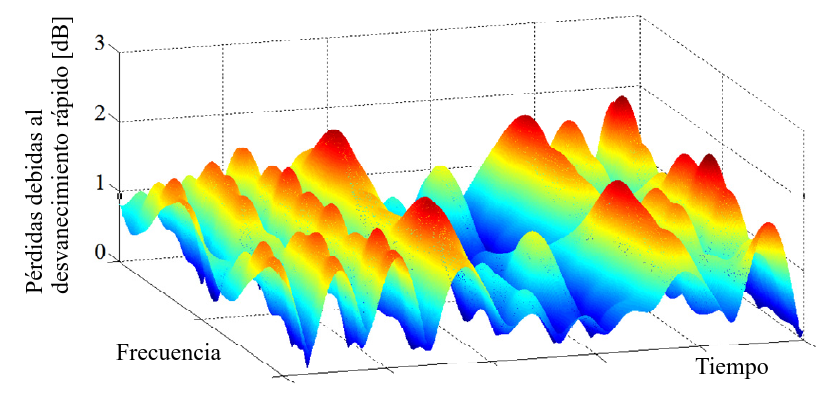
\includegraphics[height=4.0cm]{../memoria/imagenes/scheduling_italianos/scheduling_italianos-174_es.png}
\end{center}
\end{itemize}
\end{frame}

% Diapositiva
\begin{frame}
\frametitle{Fundamentos - Transmisión inalámbrica - Transmisión en el enlace radioeléctrico (V)}

\begin{center}
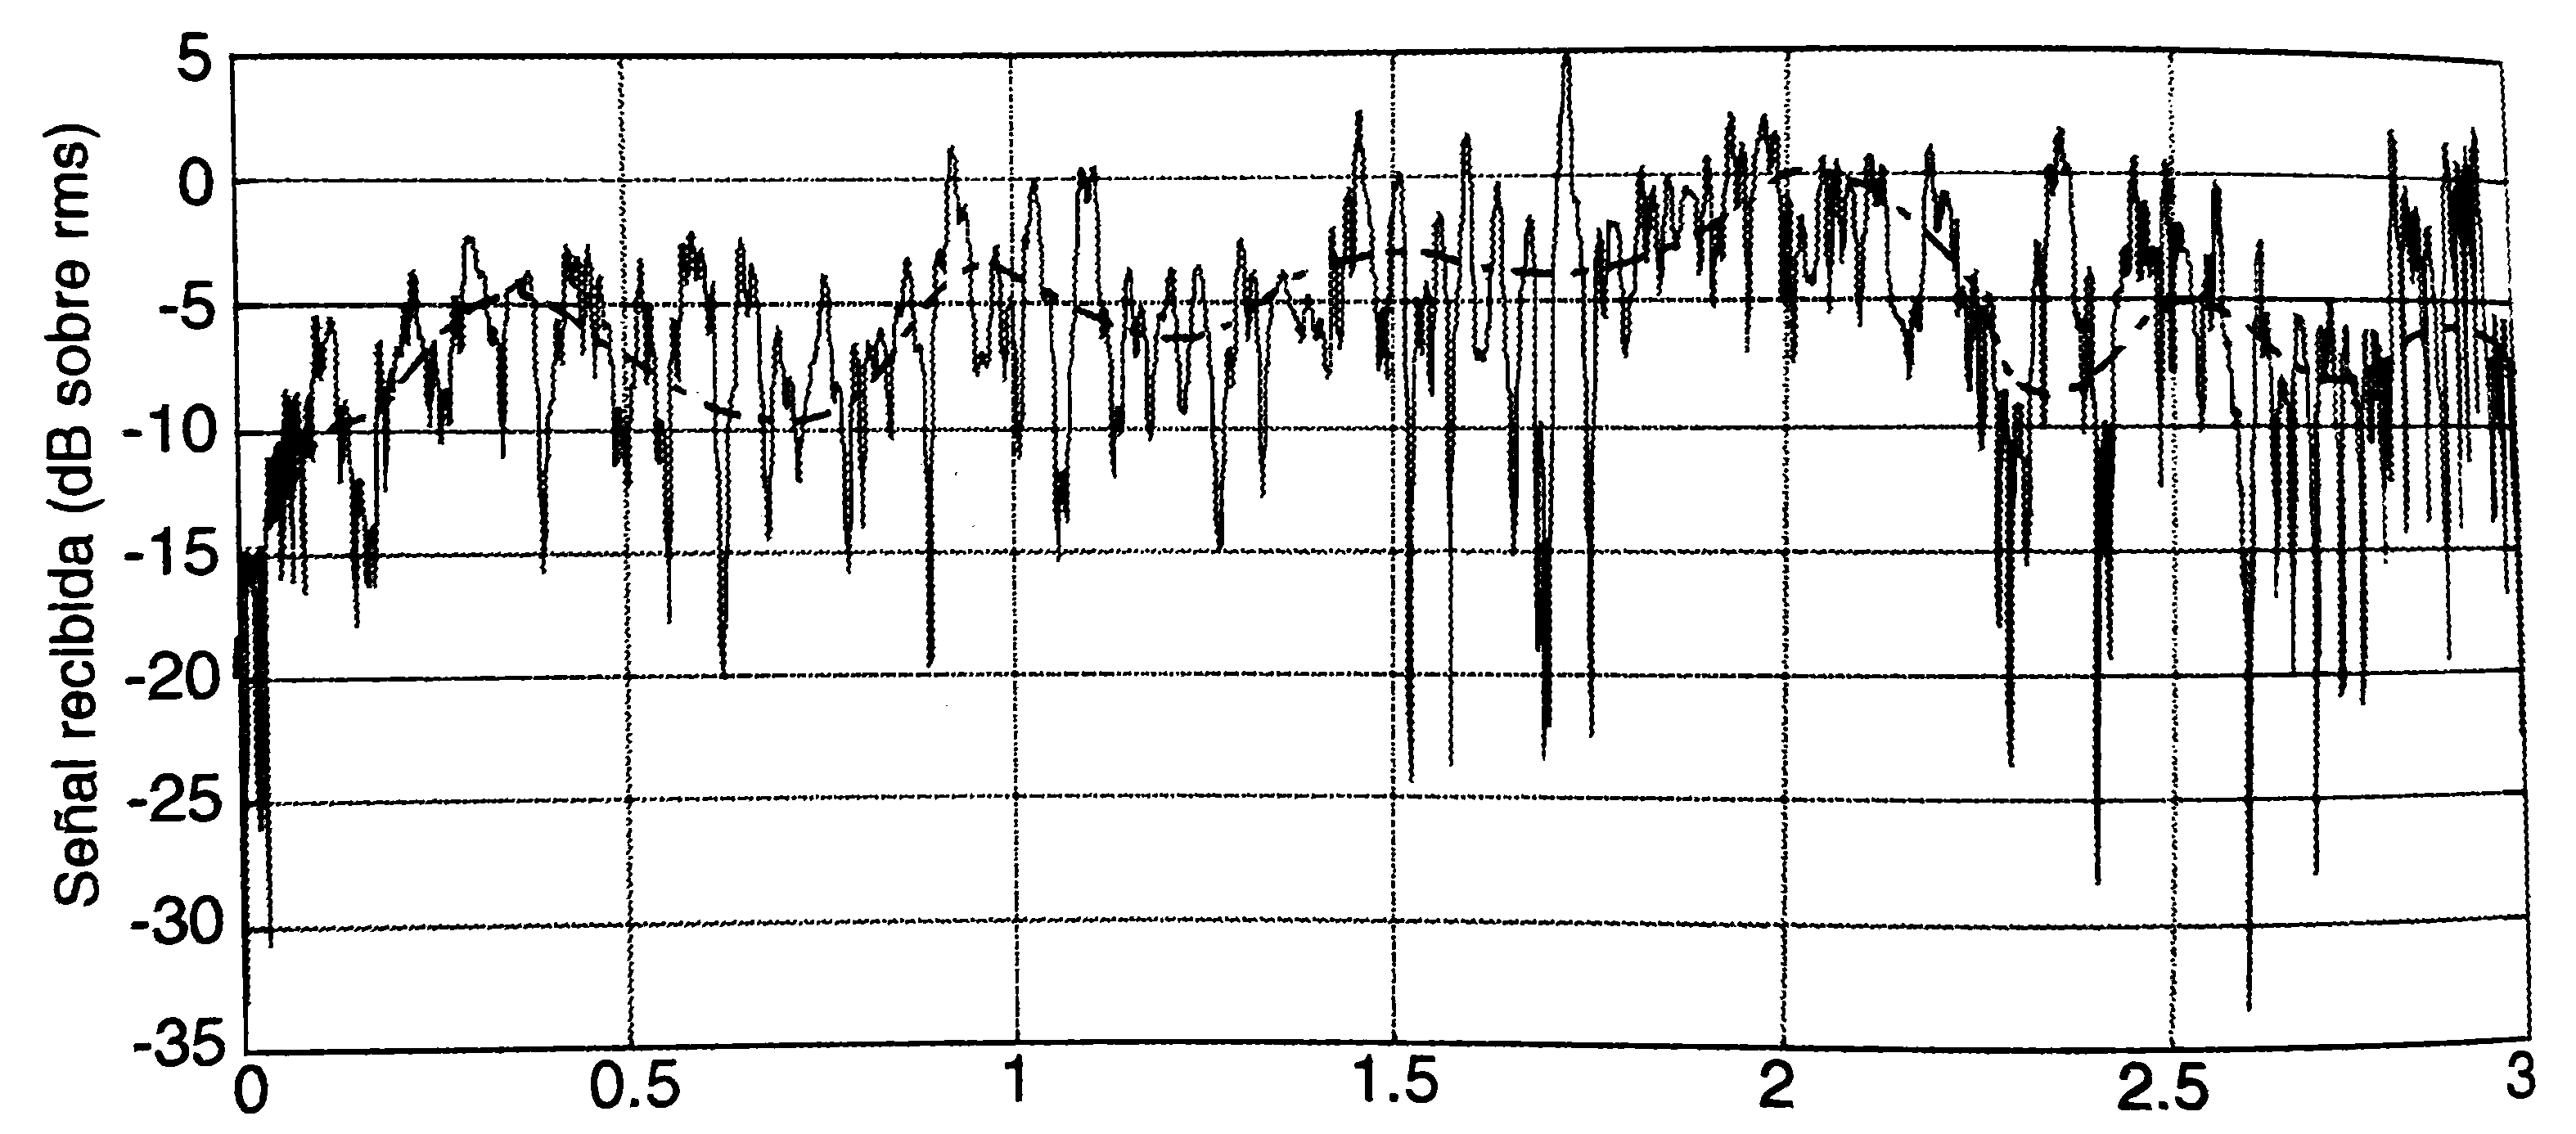
\includegraphics[height=5.0cm]{../memoria/imagenes/comunicaciones_moviles/cm_cap3_2_fixed.jpg}
\end{center}
\end{frame}

% Diapositiva
\begin{frame}
\frametitle{Fundamentos - Transmisión inalámbrica - Análisis del enlace radioeléctrico}

\begin{itemize}
\item Balance de enlace

\begin{center}
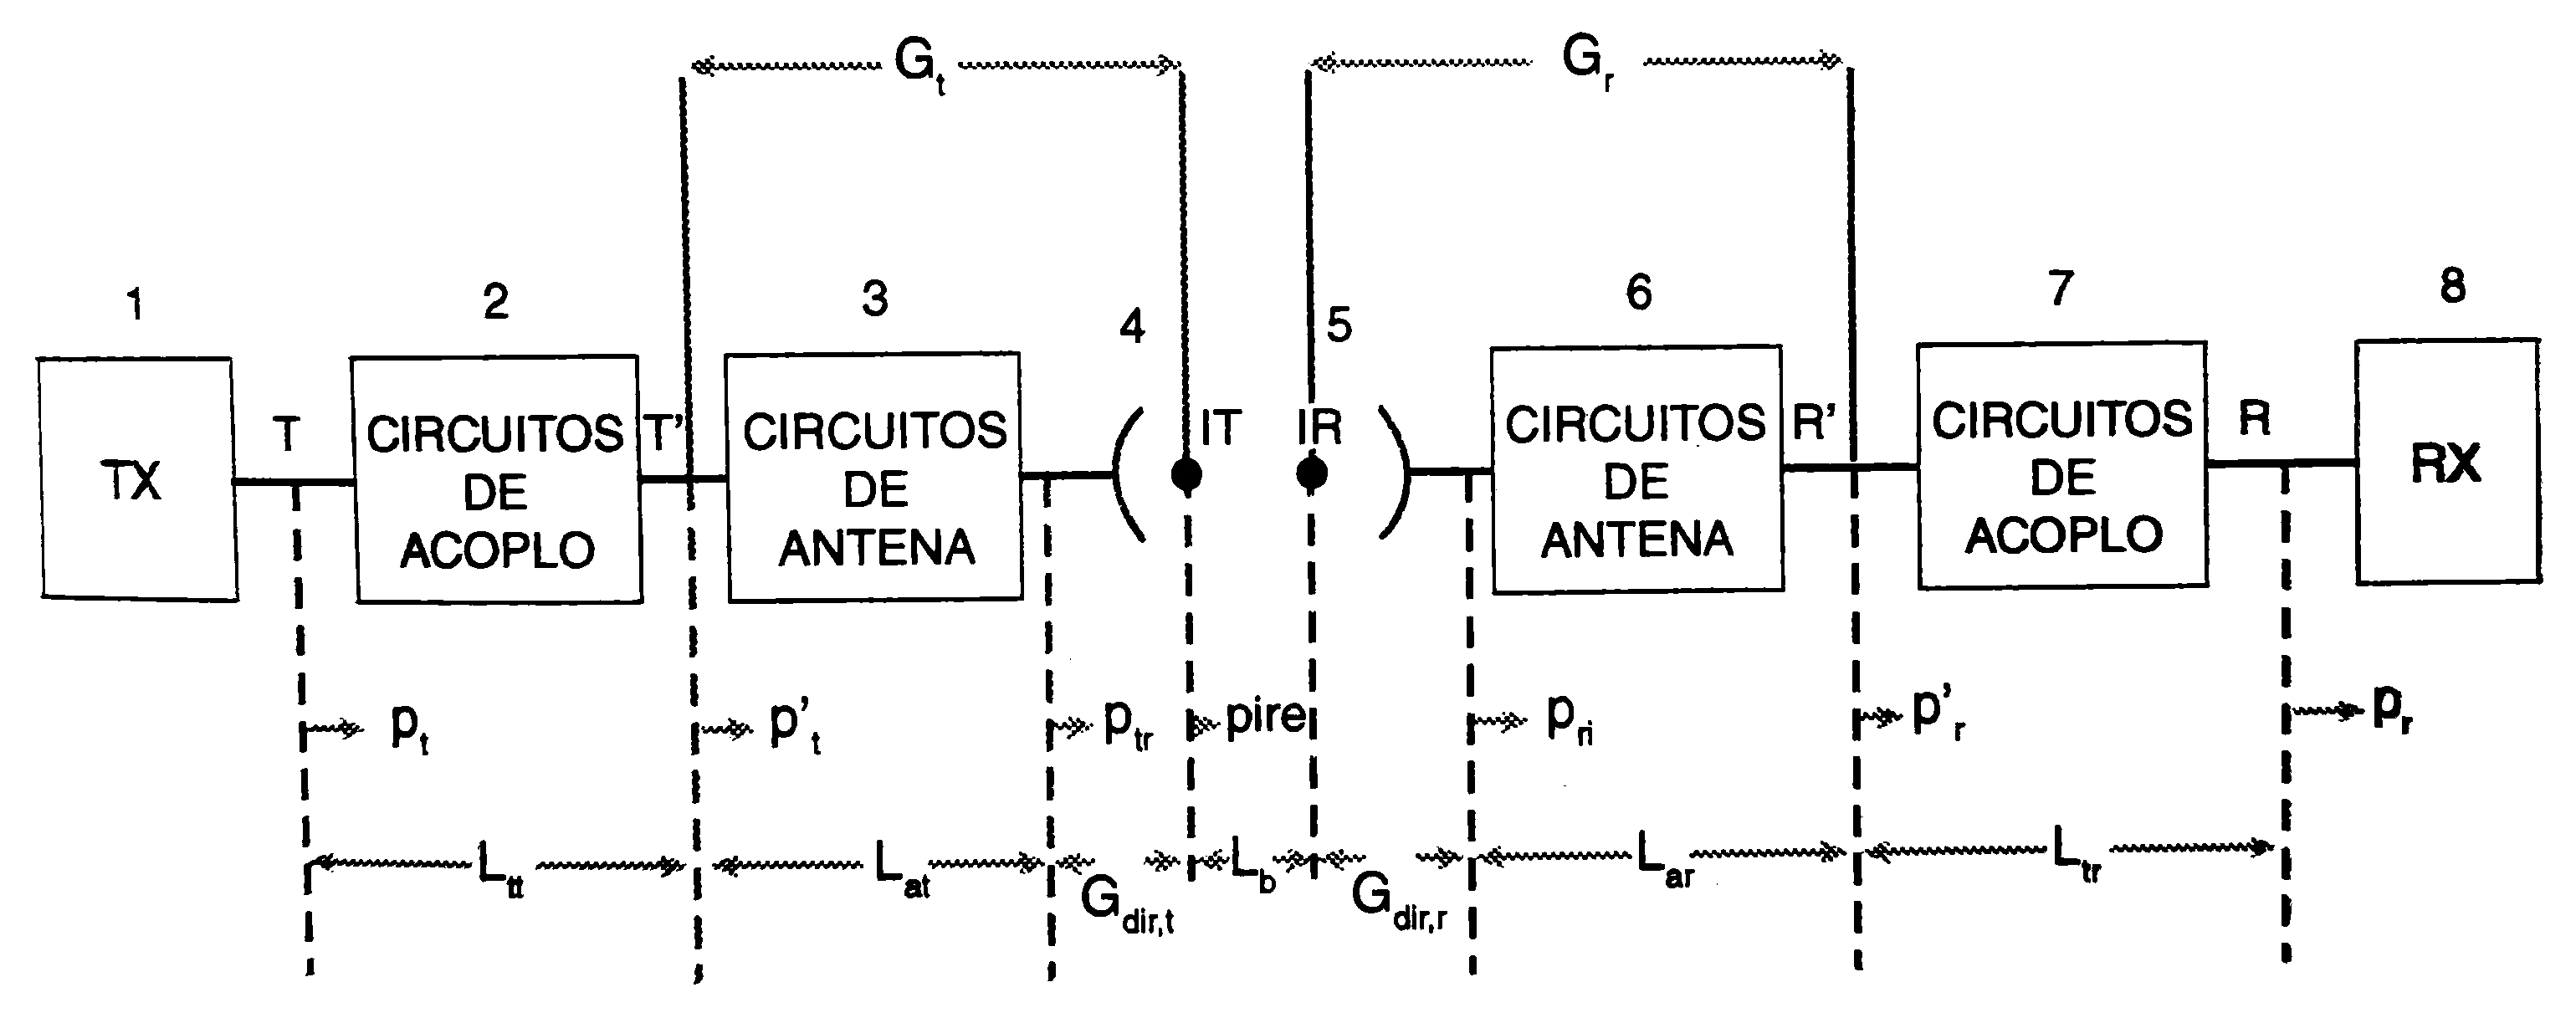
\includegraphics[height=4.0cm]{../memoria/imagenes/comunicaciones_moviles/cm_cap2_5_fixed.jpg}
\end{center}
\item {
	Modelos de canal
	\begin{itemize}
	\item Predicen la alteración de la señal transmitida.
	\item Se pueden aplicar en simuladores.
	\end{itemize}
}
\end{itemize}
\end{frame}

% Diapositiva
\begin{frame}
\frametitle{Fundamentos - Sistema celular}

\begin{itemize}
\item Una celda $\rightarrow$ Una BS.
\item Clúster $\rightarrow$ Celda $\rightarrow$ Sector
\item {
	Técnicas de \textit{reutilización de frecuencias}.
	\begin{itemize}
	\item Métodos \textit{estáticos}.
	\item Métodos \textit{dinámicos} (\textit{Inter-Cell Interference Coordination}, ICIC).
	\end{itemize}
}
\end{itemize}

\begin{center}

\includegraphics[height=5.0cm]{../memoria/imagenes/comunicaciones_moviles/cm_cap4_6_fixed_long.jpg}
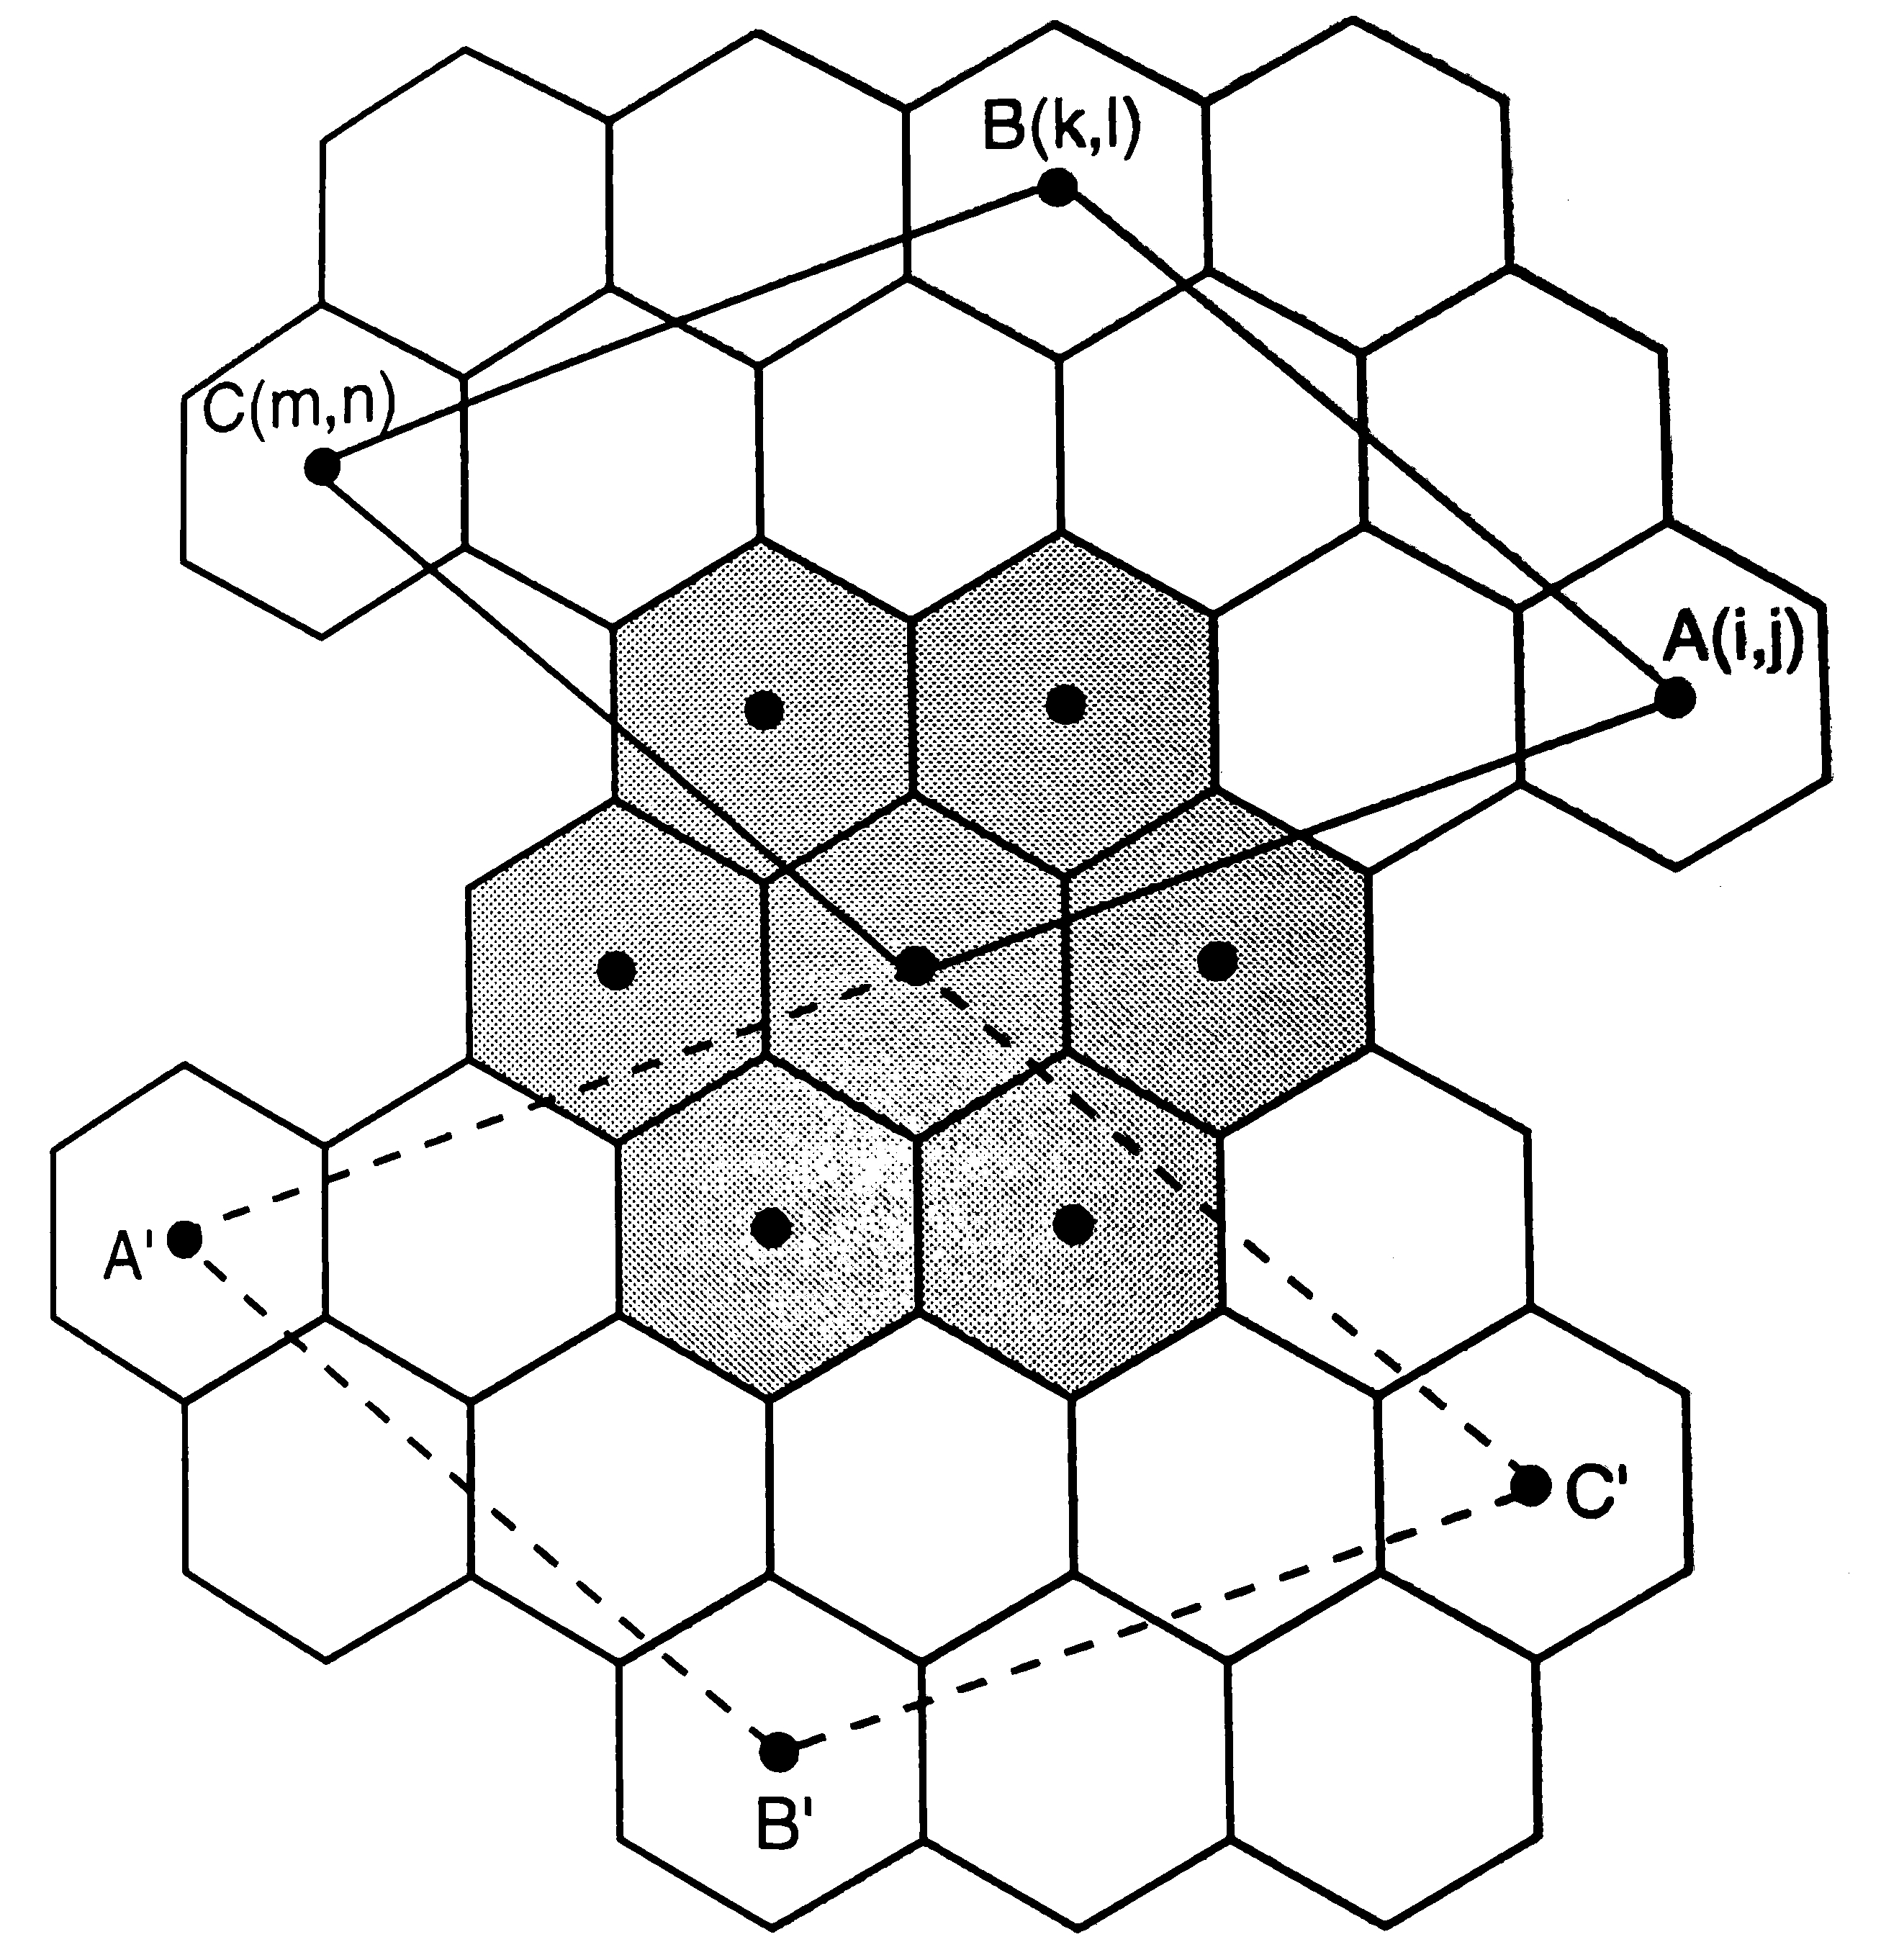
\includegraphics[height=5.0cm]{../memoria/imagenes/comunicaciones_moviles/cm_cap4_9_fixed.jpg}
\end{center}
\end{frame}

% Diapositiva
\begin{frame}
\frametitle{Fundamentos - Procesado de señal - Acceso múltiple}

\begin{itemize}
\item Los UE comparten los recursos comunes en el UL.
\item Recursos de frecuencia (FDMA).
\item Recursos de tiempo (TDMA).
\item Recursos de espacio (SDMA).
\item Recursos de código (CDMA).
\end{itemize}
\end{frame}

% Diapositiva
\begin{frame}
\frametitle{Fundamentos - Procesado de señal - Multiplexación}

\begin{itemize}
\item Los UE comparten los recursos comunes en el DL.
\item Recursos de frecuencia (FDM).
\item Recursos de tiempo (TDM).
\item Recursos de espacio (SDM).
\item Recursos de código (CDM).
\end{itemize}
\end{frame}

% Diapositiva
\begin{frame}
\frametitle{Fundamentos - Procesado de señal - Duplexación}

\begin{itemize}
\item Transmisión y recepción simultáneas.
\item Recursos de frecuencia (FDD).
\item Recursos de tiempo (TDD).
\end{itemize}
\end{frame}

% Diapositiva
\begin{frame}
\frametitle{Fundamentos - Procesado de señal - Diversidad}

\begin{itemize}
\item Dos o más versiones de la señal recibida.
\item {
	Tipos:
	\begin{itemize}
	\item De recepción: el receptor percibe dos señales separadas en recursos
	\item De transmisión: el transmisor genera dos señales separadas en recursos
	\end{itemize}
}
\item Recursos de frecuencia (FDM).
\item Recursos de tiempo (TDM).
\item Recursos de espacio (SDM).
\item Recursos de polarización. (CDM).
\end{itemize}
\end{frame}

% Diapositiva
\begin{frame}
\frametitle{Fundamentos - Procesado de señal - Modulaciones}

\begin{itemize}
\item Forma de la señal que se transmite.
\item {
	Integra diversas funcionalidades:
	\begin{itemize}
	\item Transmisión de información.
	\item Acceso múltiple.
	\item Multiplexación.
	\item Paliar diversos problemas de la transmisión inalámbrica.
	\end{itemize}
}
\item 2G y 3G: MSK, GMSK, $\pi / 4$-DPSK, M-QAM.
\item 4G y 5G: OFDM.
\end{itemize}
\end{frame}

% Diapositiva
\begin{frame}
\frametitle{Fundamentos - Procesado de señal - Codificación de canal}

\begin{itemize}
\item Se transmite una secuencia derivada de la original mediante un algoritmo.
\item Se recupera la original mediante un algoritmo complementario.
\item {
	Integra diversas funcionalidades:
	\begin{itemize}
	\item Transmisión de información.
	\item Acceso múltiple.
	\item Multiplexación.
	\item Paliar diversos problemas de la transmisión inalámbrica.
	\end{itemize}
}
\end{itemize}
\end{frame}

% Diapositiva
\begin{frame}
\frametitle{Fundamentos - Procesado de señal - Técnicas multiantena}

\begin{itemize}
\item Múltiples antenas en el transmisor y/o en el receptor.
\item El conjunto de antenas se denomina \textit{agrupación} o \textit{array}.
\item Procesado espacial: formación haz (\textit{beamforming}), codificación espacial.
\item {
	Dos modos:
	\begin{itemize}
	\item \textit{Incremento de la capacidad} / \textit{Multiplexación espacial}: Distintas señales en las distintas antenas.
	\item \textit{Diversidad espacial} / \textit{Ganancia de potencia}: Misma señal en distintas antenas.
	\end{itemize}
}
\item {
	Integra diversas funcionalidades:
	\begin{itemize}
	\item Transmisión de información.
	\item Acceso múltiple.
	\item Multiplexación.
	\item Paliar diversos problemas de la transmisión inalámbrica.
	\end{itemize}
}
\end{itemize}
\end{frame}

% Diapositiva
\begin{frame}
\frametitle{Fundamentos - Procesado de señal - Espectro ensanchado}

\begin{itemize}
\item Señal de información: $B$.
\item Señal transmitida: $W$.
\item $W > B$
\item {
	Integra diversas funcionalidades:
	\begin{itemize}
	\item Acceso múltiple.
	\item Multiplexación.
	\item Paliar diversos problemas de la transmisión inalámbrica.
	\end{itemize}
}
\end{itemize}
\end{frame}

% Diapositiva
\begin{frame}
\frametitle{Fundamentos - Otras técnicas avanzadas - Básico}

\begin{itemize}
\item Presentes en los sistemas de tercera generación en adelante.
\item Abarcan varios niveles de la pila de protocolos.
\item Destacan las técnicas de gestión de RRM.
\end{itemize}
\end{frame}

% Diapositiva
\begin{frame}
\frametitle{Fundamentos - Otras técnicas avanzadas - HARQ}

\begin{itemize}
\item Caso de RRM.
\item La señal se divide en bloques y se usa corrección y detección en cada bloque por separado.
\item \textit{HARQ con combinación de retransmisiones}.
\end{itemize}
\end{frame}

% Diapositiva
\begin{frame}
\frametitle{Fundamentos - Otras técnicas avanzadas - Planificación de paquetes o planificación de usuarios}

\begin{itemize}
\item Caso de RRM.
\item La red que controla a qué usuario se transmite (DL) o se le permite transmitir (UL) dentro de los canales compartidos.
\item En la modulación OFDM, los recursos son de tiempo y frecuencia.
\end{itemize}
\end{frame}

% Diapositiva
\begin{frame}
\frametitle{Fundamentos - Otras técnicas avanzadas - Adaptación de enlace}

\begin{itemize}
\item Caso de RRM.
\item Se modifican los parámetros de la transmisión (potencia, modulación, tasa de codificación de canal) en función del estado del canal.
\item Se persigue un objetivo: maximizar la tasa binaria neta, conseguir una tasa binaria fija con un retardo acotado, etc.
\item {
	En los modernos sistemas de comunicaciones móviles:
	\begin{itemize}
	\item Variar la tasa binaria (AMC).
	\item Modificar la modulación y la tasa de codificación de canal (MCS).
	\item Se tiene información sobre el estado del canal (CQI) de cada usuario.
	\end{itemize}
}
\end{itemize}
\end{frame}

% Diapositiva
\begin{frame}
\frametitle{Fundamentos - Otras técnicas avanzadas - Categoría de terminal}

\begin{itemize}
\item Caso de RRM.
\item Diferentes categorías de terminales en función de qué características incluyen.
\item {
	En los sistemas de comunicaciones móviles de cuarta generación:
	\begin{itemize}
	\item Capacidad de transmisión/recepción de datos.
	\item Tamaño del \textit{buffer} de recepción para HARQ.
	\item Número de capas de multiplexación espacial.
	\end{itemize}
}
\end{itemize}
\end{frame}

% Diapositiva
\begin{frame}
\frametitle{Fundamentos - Otras técnicas avanzadas - Agregación de portadoras}

\begin{itemize}
\item Se logran mayores anchuras agregando portadoras independientes (\textit{component carrier}) de ancho $b_i$:
$$B = \sum_i b_i$$
\item Aumenta la capacidad.
\end{itemize}
\end{frame}

% Diapositiva
\begin{frame}
\frametitle{Fundamentos - Otras técnicas avanzadas - MIMO avanzado}

\begin{itemize}
\item {
	\textit{Release 8}:
	\begin{itemize}
	\item Diversidad en transmisión en el DL mediante SFBC con dos antenas en el transmisor $\rightarrow$ SFBC, SFBC combinado con FSTD.
	\item Multiplexación espacial en el DL con hasta cuatro capas.
	\item Multiplexación espacial en el DL con una capa (formación de haz) $\rightarrow$ \textit{Codebook-based beamforming}.
	\item Diferentes capas asignadas a distintos terminales (MIMO multiusuario).
	\end{itemize}
}
\item {
	\textit{Release 10}:
	\begin{itemize}
	\item Multiplexación espacial en el DL con hasta ocho capas.
	\item Multiplexación espacial en el UL con hasta cuatro capas.
	\end{itemize}
}
\end{itemize}
\end{frame}

% Diapositiva
\begin{frame}
\frametitle{Fundamentos - Otras técnicas avanzadas - Redes heterogéneas}

\begin{itemize}
\item Complementar una macrocelda (gran capacidad, gran área de cobertura) con varias picoceldas (baja potencia).
\item El resultado es una red heterogénea (\textit{HetNet}).
\end{itemize}
\end{frame}

% Diapositiva
\begin{frame}
\frametitle{Fundamentos - Otras técnicas avanzadas - Nodos repetidores}

\begin{itemize}
\item Estaciones base de baja potencia que se conectan a un eNB convencional
\item En DL, reciben la del eNB y la retransmiten a su zona de cobertura.
\item En UL, los repetidores captan la señal de los móviles y la retransmiten al eNB.
\end{itemize}
\end{frame}

% Diapositiva
\begin{frame}
\frametitle{Fundamentos - Otras técnicas avanzadas - Transmisión multipunto coordinada}

\begin{itemize}
\item Aumento de la tasa binaria en el borde de la célula $\rightarrow$ Aumento de la tasa binaria media en la célula.
\item El UE situado en el borde se puede conectar con dos o más eNB.
\item En la misma celda y diferentes sectores (CoMP intracelular).
\item En diferentes celdas (CoMP intercelular).
\end{itemize}
\end{frame}

% Diapositiva
\begin{frame}
\frametitle{Fundamentos - Otras técnicas avanzadas - Novedades de 5G}

\begin{itemize}
\item Seccionamiento de la red (\textit{Network Slicing}). $\rightarrow$ No tiene repercusión en el funcionamiento de la interfaz de radio.
\item Virtualización de funciones de red (\textit{Network Function Virtualization}, NFV). $\rightarrow$ Mismas funcionalidades básicas de la interfaz de radio.
\item Computación en el borde de la red (\textit{Multi-access Edge Computing}, MEC). $\rightarrow$ No tiene repercusión en el funcionamiento de la interfaz de radio.
\end{itemize}
\end{frame}

% SUBSECCIÓN
\subsection{Interfaz de radio de 5G}

% Diapositiva
\begin{frame}
\frametitle{NR - Básico}

\begin{itemize}
\item La interfaz de radio de 5G se denomina NR (\textit{New Radio}).
\item NR toma todos los fundamentos concebidos para 2G, 3G, 4G.
\item Nuevos servicios:  eMBB, CC, URLLC, mIoT, \textit{Flexible network operations}.
\end{itemize}
\end{frame}

% % Diapositiva
% \begin{frame}
% \frametitle{NR - Arquitectura de la red}
%
% \begin{itemize}
% \item {
% 	Elementos:
% 	\begin{itemize}
% 	\item \textit{User Equipment}, UE
% 	\item {
% 		\textit{New Generation Radio Access Network}, NG-RAN $\rightarrow$ \textit{5G Node B}, gNB
% 		\begin{itemize}
% 		\item \textit{gNB-Central Unit}, gNB-CU
% 		\item \textit{gNB-Distributed Unit}, gNB-DU
% 		\end{itemize}
% 	}
% 	\item {
% 		\textit{5G Core Network}, 5GC
% 		\begin{itemize}
% 		\item \textit{User Plane Function}, UPF
% 		\item \textit{Access and Mobility management Function}, AMF
% 		\end{itemize}
% 	}
% 	\end{itemize}
%
% 	\begin{center}
% 	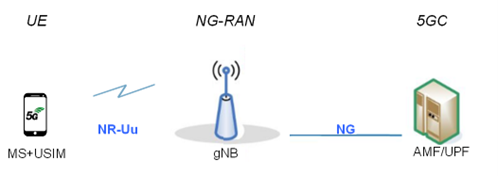
\includegraphics[height=3.5cm]{../memoria/imagenes/3gpp_5g_system_overview/5g-fig1.png}
% 	\end{center}
% }
% \item {
% 	Arquitectura basada en servicios (\textit{Service-Based Architecture}, SBA):
% 	\begin{itemize}
% 	\item Funciones de red (Network Functions, NF).
% 	\item Modularidad y reusabilidad.
% 	\end{itemize}
% }
% \item {
% 	Interfaces relacionadas con la interfaz de radio:
% 	\begin{itemize}
% 	\item \textit{New Radio Uu}, NR-Uu.
% 	\item F1.
% 	\item \textit{NG} $\rightarrow$ Constituido por varias interfaces, como N2 ó N3.
% 	\end{itemize}
%
% 	\begin{center}
% 	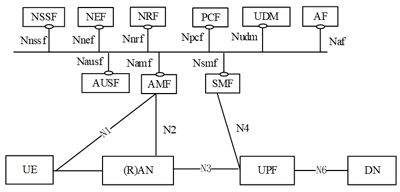
\includegraphics[height=5.0cm]{../memoria/imagenes/3gpp_5g_system_overview/5g-fig2.png}
% 	\end{center}
% }
% \item Se usan canales físicos y señales físicas.
% \item {
% 	Protocolos relacionados con la interfaz de radio:
% 	\begin{enumerate}
% 	\item {
% 		La capa física o \textit{capa PHY} (\textit{PHY layer}):
% 		\begin{itemize}
% 		\item Transmitir y recibir señal por el canal de radio.
% 		\item Informes CQI.
% 		\end{itemize}
% 	}
% 	\item {
% 		La capa de enlace o \textit{capa MAC} (\textit{MAC layer}):
% 		\begin{itemize}
% 		\item RRM
% 		\end{itemize}
% 	}
% 	\item {
% 		La capa de red o \textit{capa PDCP/RLC} (\textit{PDCP/RLC layer}):
% 		\begin{itemize}
% 		\item Maneja los paquetes IP.
% 		\end{itemize}
% 	}
% 	\end{enumerate}
% }
% \item {
% 	Modos de despliegue:
% 	\begin{itemize}
% 	\item {
% 		\textit{Non-Stand Alone}, NSA:
% 		\begin{itemize}
% 		\item NG-RAN, NR + E-UTRAN, EPC
% 		\item Despliegue paulatino de 5G
% 		\item servicios de 4G, pero se pueden apreciar las capacidades de NR.
% 		\end{itemize}
%
% 		\begin{center}
% 		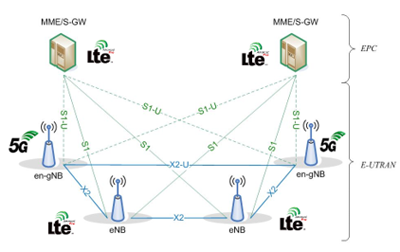
\includegraphics[height=5.0cm]{../memoria/imagenes/3gpp_5g_system_overview/5g-fig5.png}
% 		\end{center}
% 	}
% 	\item {
% 		\textit{Stand-Alone}, SA:
% 		\begin{itemize}
% 		\item NG-RAN, NR + 5GC.
% 		\item Servicios de 5G, se aprecian todas sus capacidades las capacidades de NR.
% 		\end{itemize}
%
% 		\begin{center}
% 		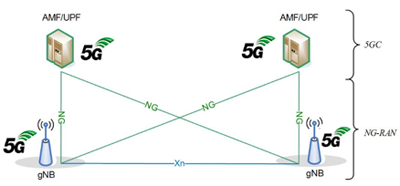
\includegraphics[height=5.0cm]{../memoria/imagenes/3gpp_5g_system_overview/5g-fig6.png}
% 		\end{center}
% 	}
% 	\end{itemize}
% }
% \end{itemize}
% \end{frame}

% Diapositiva
\begin{frame}
\frametitle{NR - Arquitectura de la red (I)}

\begin{itemize}
\item {
	Elementos:
	\begin{itemize}
	\item \textit{User Equipment}, UE
	\item {
		\textit{New Generation Radio Access Network}, NG-RAN $\rightarrow$ \textit{5G Node B}, gNB
		\begin{itemize}
		\item \textit{gNB-Central Unit}, gNB-CU
		\item \textit{gNB-Distributed Unit}, gNB-DU
		\end{itemize}
	}
	\item {
		\textit{5G Core Network}, 5GC
		\begin{itemize}
		\item \textit{User Plane Function}, UPF
		\item \textit{Access and Mobility management Function}, AMF
		\end{itemize}
	}
	\end{itemize}

	\begin{center}
	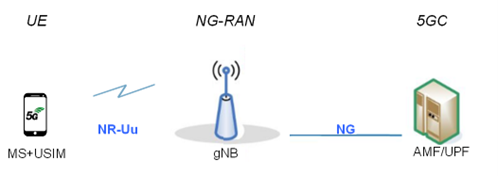
\includegraphics[height=2.5cm]{../memoria/imagenes/3gpp_5g_system_overview/5g-fig1.png}
	\end{center}
}
\item {
	Arquitectura basada en servicios (\textit{Service-Based Architecture}, SBA):
	\begin{itemize}
	\item Funciones de red (Network Functions, NF).
	\item Modularidad y reusabilidad.
	\end{itemize}
}
\end{itemize}
\end{frame}

% Diapositiva
\begin{frame}
\frametitle{NR - Arquitectura de la red (II)}

\begin{itemize}
\item {
	Interfaces relacionadas con la interfaz de radio:
	\begin{itemize}
	\item \textit{New Radio Uu}, NR-Uu.
	\item F1.
	\item \textit{NG} $\rightarrow$ Constituido por varias interfaces, como N2 ó N3.
	\end{itemize}

	\begin{center}
	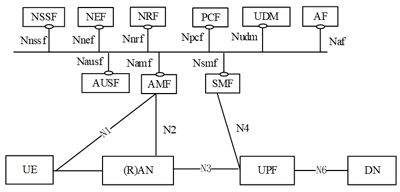
\includegraphics[height=3.5cm]{../memoria/imagenes/3gpp_5g_system_overview/5g-fig2.png}
	\end{center}
}
\item Se usan canales físicos y señales físicas.
\end{itemize}
\end{frame}

% Diapositiva
\begin{frame}
\frametitle{NR - Arquitectura de la red (III)}

\begin{itemize}
\item {
	Protocolos relacionados con la interfaz de radio:
	\begin{enumerate}
	\item {
		La capa física o \textit{capa PHY} (\textit{PHY layer}):
		\begin{itemize}
		\item Transmitir y recibir señal por el canal de radio.
		\item Informes CQI.
		\end{itemize}
	}
	\item {
		La capa de enlace o \textit{capa MAC} (\textit{MAC layer}):
		\begin{itemize}
		\item RRM
		\end{itemize}
	}
	\item {
		La capa de red o \textit{capa PDCP/RLC} (\textit{PDCP/RLC layer}):
		\begin{itemize}
		\item Maneja los paquetes IP.
		\end{itemize}
	}
	\end{enumerate}
}
\end{itemize}
\end{frame}

% Diapositiva
\begin{frame}
\frametitle{NR - Arquitectura de la red (IV)}

\begin{itemize}
\item {
	Modos de despliegue:
	\begin{itemize}
	\item {
		\textit{Non-Stand Alone}, NSA:
		\begin{itemize}
		\item NG-RAN, NR + E-UTRAN, EPC
		\item Despliegue paulatino de 5G
		\item servicios de 4G, pero se pueden apreciar las capacidades de NR.
		\end{itemize}

		\begin{center}
		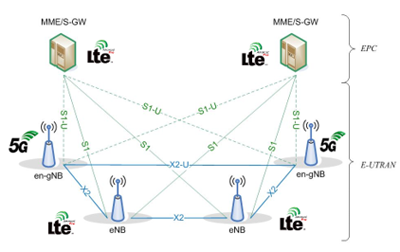
\includegraphics[height=5.0cm]{../memoria/imagenes/3gpp_5g_system_overview/5g-fig5.png}
		\end{center}
	}
	\end{itemize}
}
\end{itemize}
\end{frame}

% Diapositiva
\begin{frame}
\frametitle{NR - Arquitectura de la red (V)}

\begin{itemize}
\item {
	\begin{itemize}
	\item {
		\textit{Stand-Alone}, SA:
		\begin{itemize}
		\item NG-RAN, NR + 5GC.
		\item Servicios de 5G, se aprecian todas sus capacidades las capacidades de NR.
		\end{itemize}

		\begin{center}
		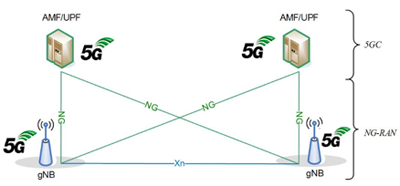
\includegraphics[height=4.5cm]{../memoria/imagenes/3gpp_5g_system_overview/5g-fig6.png}
		\end{center}
	}
	\end{itemize}
}
\end{itemize}
\end{frame}

% Diapositiva
\begin{frame}
\frametitle{NR - Transmisión inalámbrica}

\begin{itemize}
\item Todos los fenómenos descritos.
\item Avanzados modelos de canal para poder simular fenómenos como la atenuación, el desvanecimiento lento y el desvanecimiento rápido.
\end{itemize}
\end{frame}

% Diapositiva
\begin{frame}
\frametitle{NR - Sistema celular}

\begin{itemize}
\item Usa un sistema celular moderno, con estaciones repartidas para dar cobertura.
\item HetNet
\item RN
\item CoMP
\item {
	Frecuencias:
	\begin{itemize}
	\item Las portadoras van de 400 MHz a 100 GHz.
	\item Las bandas licenciadas van de 600 MHz a 39 GHz.
	\item {
		Tres rangos:
		\begin{itemize}
		\item Hasta 1 GHz: Mejor propagación (despliegues rurales).
		$B \leq 100$ MHz
		\item De 1 GHz a 6 GHz: Despliegues urbanos y suburbanos.
		$B \leq 100$ MHz
		\item A partir de 6 GHz: Peor propagación (\textit{hot-spot}).
		$B \leq 400$ MHz
		\end{itemize}
	}
	\end{itemize}
}
\end{itemize}
\end{frame}

% % Diapositiva
% \begin{frame}
% \frametitle{NR - Procesado de señal - Modulaciones}
%
% \begin{itemize}
% \item {
% 	Uso de OFDM:
% 	\begin{itemize}
% 	\item DL: OFDM con prefijo cíclico.
% 	\item UL: \textit{OFDM con precodificación de transformada discreta de Fourier} (DFT-s-OFDM).
% 	\end{itemize}
% }
% \item {
% 	Malla de recursos de tiempo-frecuencia
% 	\begin{itemize}
% 	\item {
% 		La malla se divide en:
% 		\begin{itemize}
% 		\item Frecuencia: trama, \textit{Resource Block} (RB), subportadora.
% 		\item Tiempo: trama, subtrama, \textit{slot}.
% 		\end{itemize}
%
% 		\begin{center}
% 		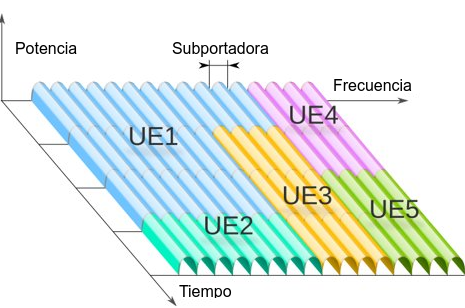
\includegraphics[height=2.5cm]{../memoria/imagenes/fikore_doc/figures/Grid_es.png}
% 		\end{center}
% 	}
% 	\item Gran flexibilidad y granularidad: \textit{Resource Element} (RE), \textit{Physical Resource Blocks} (PRB), \textit{Resource Block Groups} (RBG).
% 	\item {
% 		Numerología:
%
% 		\begin{center}
% 		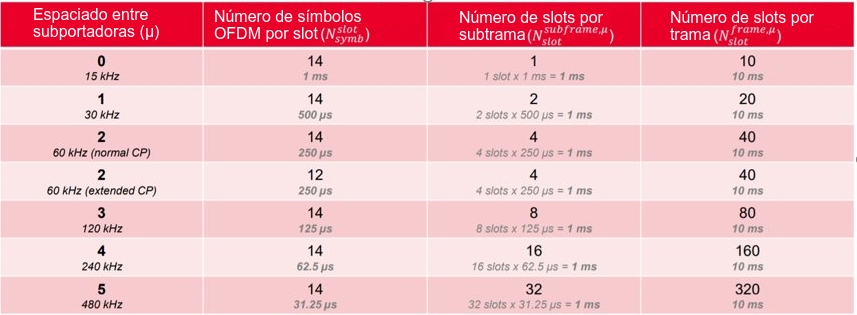
\includegraphics[height=2.5cm]{../memoria/imagenes/fikore_doc/figures/Numerology_es.png}
% 		\end{center}
% 	}
% 	\item {
% 		Modulaciones: QPSK (2 bits), 16-QAM (4 bits), 64-QAM (6 bits), 256-QAM (8 bits).
% 		AMC.
% 	}
% 	\item \textit{Transport Block Size} (TBS).
% 	\item Transmisión dúplex.
% 	\item {
% 		Uso de canales físicos y señales físicas.
%
% 		\begin{center}
% 		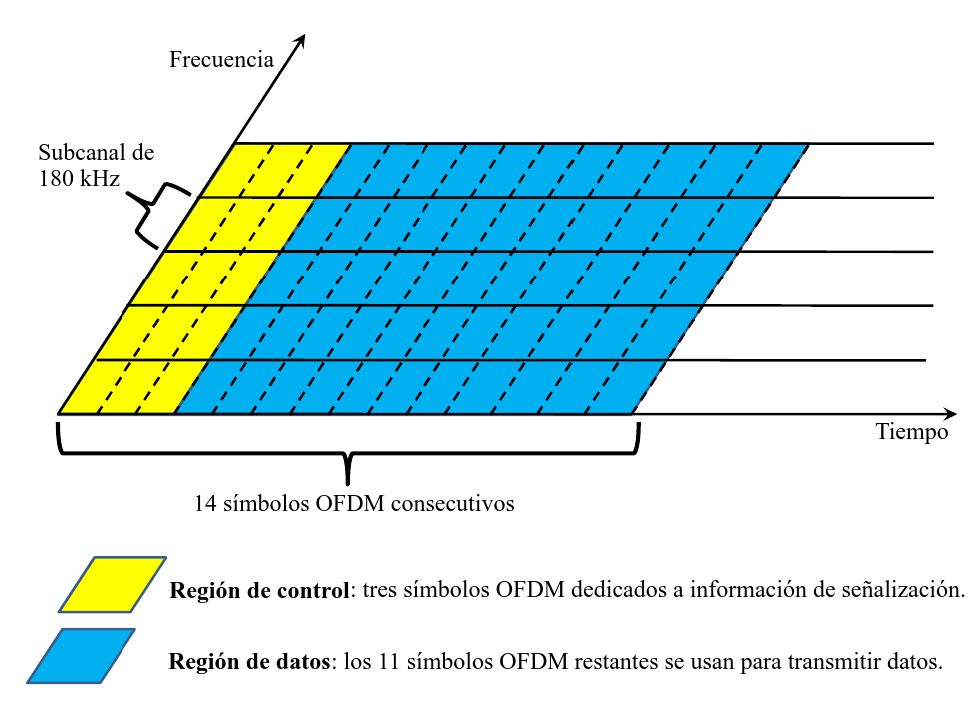
\includegraphics[height=2.5cm]{../memoria/imagenes/scheduling_italianos/scheduling_italianos-173_es.png}
% 		\end{center}
% 	}
% 	\end{itemize}
% }
% \end{itemize}
% \end{frame}

% Diapositiva
\begin{frame}
\frametitle{NR - Procesado de señal - Modulaciones (I)}

\begin{itemize}
\item {
	Uso de OFDM:
	\begin{itemize}
	\item DL: OFDM con prefijo cíclico.
	\item UL: \textit{OFDM con precodificación de transformada discreta de Fourier} (DFT-s-OFDM).
	\end{itemize}
}
\item {
	Malla de recursos de tiempo-frecuencia
	\begin{itemize}
	\item {
		La malla se divide en:
		\begin{itemize}
		\item Frecuencia: trama, \textit{Resource Block} (RB), subportadora.
		\item Tiempo: trama, subtrama, \textit{slot}.
		\end{itemize}

		\begin{center}
		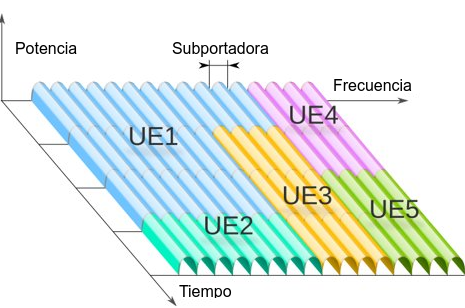
\includegraphics[height=3.5cm]{../memoria/imagenes/fikore_doc/figures/Grid_es.png}
		\end{center}
	}
	\end{itemize}
}
\end{itemize}
\end{frame}

% Diapositiva
\begin{frame}
\frametitle{NR - Procesado de señal - Modulaciones (II)}

\begin{itemize}
\item {
	\begin{itemize}
	\item Gran flexibilidad y granularidad: \textit{Resource Element} (RE), \textit{Physical Resource Blocks} (PRB), \textit{Resource Block Groups} (RBG).
	\item {
		Numerología:

		\begin{center}
		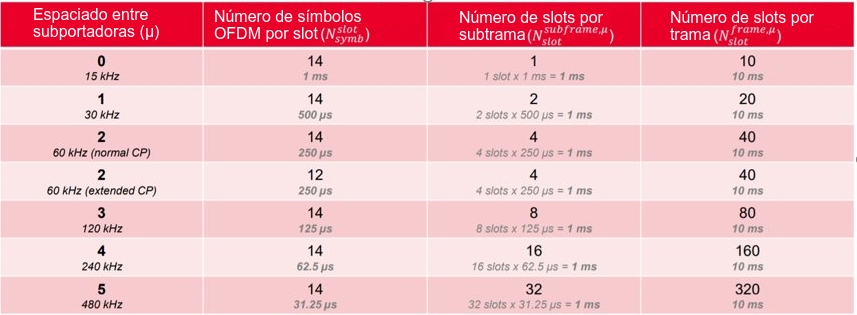
\includegraphics[height=3.5cm]{../memoria/imagenes/fikore_doc/figures/Numerology_es.png}
		\end{center}
	}
	\item {
		Modulaciones: QPSK (2 bits), 16-QAM (4 bits), 64-QAM (6 bits), 256-QAM (8 bits).
		AMC.
	}
	\item \textit{Transport Block Size} (TBS).
	\item Transmisión dúplex.
	\end{itemize}
}
\end{itemize}
\end{frame}

% Diapositiva
\begin{frame}
\frametitle{NR - Procesado de señal - Modulaciones (III)}

\begin{itemize}
\item {
	\begin{itemize}
	\item {
		Uso de canales físicos y señales físicas.

		\begin{center}
		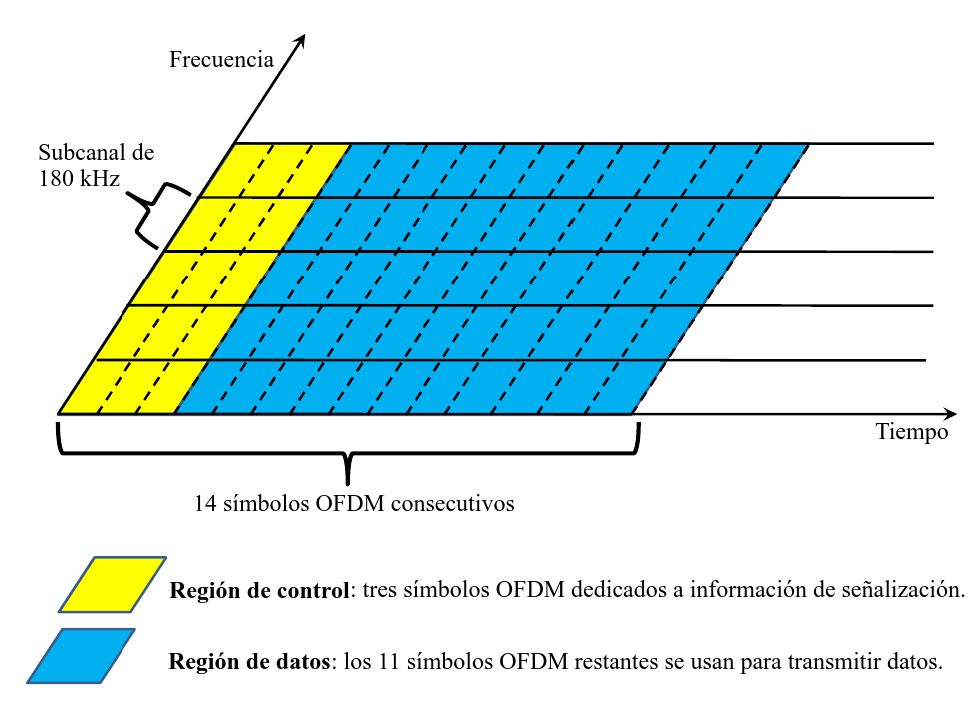
\includegraphics[height=5.5cm]{../memoria/imagenes/scheduling_italianos/scheduling_italianos-173_es.png}
		\end{center}
	}
	\end{itemize}
}
\end{itemize}
\end{frame}

% Diapositiva
\begin{frame}
\frametitle{NR - Procesado de señal - MIMO}

\begin{itemize}
\item 5G incorpora mejoras de las técnicas multiantena de \textit{LTE-Advanced}.
\item Nueva modalidad: MIMO \textit{Over-the-Air} (OTA).
\end{itemize}
\end{frame}

% Diapositiva
\begin{frame}
\frametitle{NR - Otras técnicas avanzadas}

\begin{itemize}
\item HARQ.
\item Planificación de paquetes.
\item Adaptación de enlace.
\item Agregación de portadoras.
\end{itemize}
\end{frame}

% SUBSECCIÓN
\subsection{Emulación del acceso radio 5G}

% Diapositiva
\begin{frame}
\frametitle{Emulación del acceso radio 5G - Aspectos}

\begin{itemize}
\item Arquitectura (descripción funcional, protocolos e interfaces). $\rightarrow$ Sistemas informáticos.
\item {
	Transmisión inalámbrica:
	\begin{itemize}
	\item Transmisión de señales. $\rightarrow$ Teoría de la comunicación.
	\item Ruido e interferencia. $\rightarrow$ Estadística, modelos de canal, balances de enlace.
	\item {
		Canal de transmisión. $\rightarrow$ Teoría de simulación de sistemas de comunicaciones.
		\begin{itemize}
		\item Desvanecimiento rápido. $\rightarrow$ Los sistemas lineales variantes en el tiempo.
		\item Desvanecimiento lento y la atenuación. $\rightarrow$ Los sistemas lineales invariantes en el tiempo.
		\item Amplificadores. $\rightarrow$ Los sistemas no lineales.
		\end{itemize}
	}
	\end{itemize}
}
\item Parámetros del sistema. $\rightarrow$ Monte Carlo, muestreo enfatizado, etc.
\end{itemize}
\end{frame}

% Diapositiva
\begin{frame}
\frametitle{Emulación del acceso radio 5G - Emuladores y simuladores}

\begin{itemize}
\item {
	Simuladores de RAN:
	\begin{itemize}
	\item Permiten estudiar las prestaciones de un despliegue de la red de 5G.
	\item \textit{Vienna Simulator}, \textit{NS-3}, \textit{Matlab 5G Toolbox}, \textit{5G-LENA}.
	\end{itemize}
}
\item {
	Emuladores de RAN de nivel de sistema:
	\begin{itemize}
	\item Permite estudiar directamente el rendimiento de una aplicación de 5G en un despliegue simulado.
	\item Extensión de \textit{NS-3}, \textit{OpenAirInterface 5G-RAN}, \textit{Simu5G}, \textit{Polaris}, \textit{Keysight}, \textit{FikoRE}.
	\end{itemize}
}
\end{itemize}
\end{frame}





\section{Emulador \textit{FikoRE}}

% Diapositiva
\begin{frame}
\frametitle{Emulador \textit{FikoRE} - Básico}

\begin{itemize}
\item \textit{Framework for Immersive communication networK Optimization RAN Emulator} (\textit{FikoRE}).
\item Emulador de nivel de sistema de la interfaz de radio de 5G.
\item Recrea la interfaz de radio (PHY, MAC, PDCP/RLC).
\end{itemize}
\end{frame}

\subsection{Características generales}

% Diapositiva
\begin{frame}
\frametitle{Emulador \textit{FikoRE} - Características generales - Implementación}

\begin{itemize}
\item \textit{C++}
\item \textit{Linux}
\item {
	Clases:
	\begin{itemize}
	\item {
		Terminal de usuario (UE):
		\begin{itemize}
		\item PHY.
		\item PDCP/RLC.
		\item Movilidad del UE.
		\item Manejo de paquetes (captura, generación).
		\item Otros comportamientos del UE.
		\end{itemize}
	}
	\item {
		Estación base (gNB):
		\begin{itemize}
		\item MAC.
		\end{itemize}
	}
	\end{itemize}
}
\end{itemize}
\end{frame}

% Diapositiva
\begin{frame}
\frametitle{Emulador \textit{FikoRE} - Características generales - Flujo de información}

\begin{center}
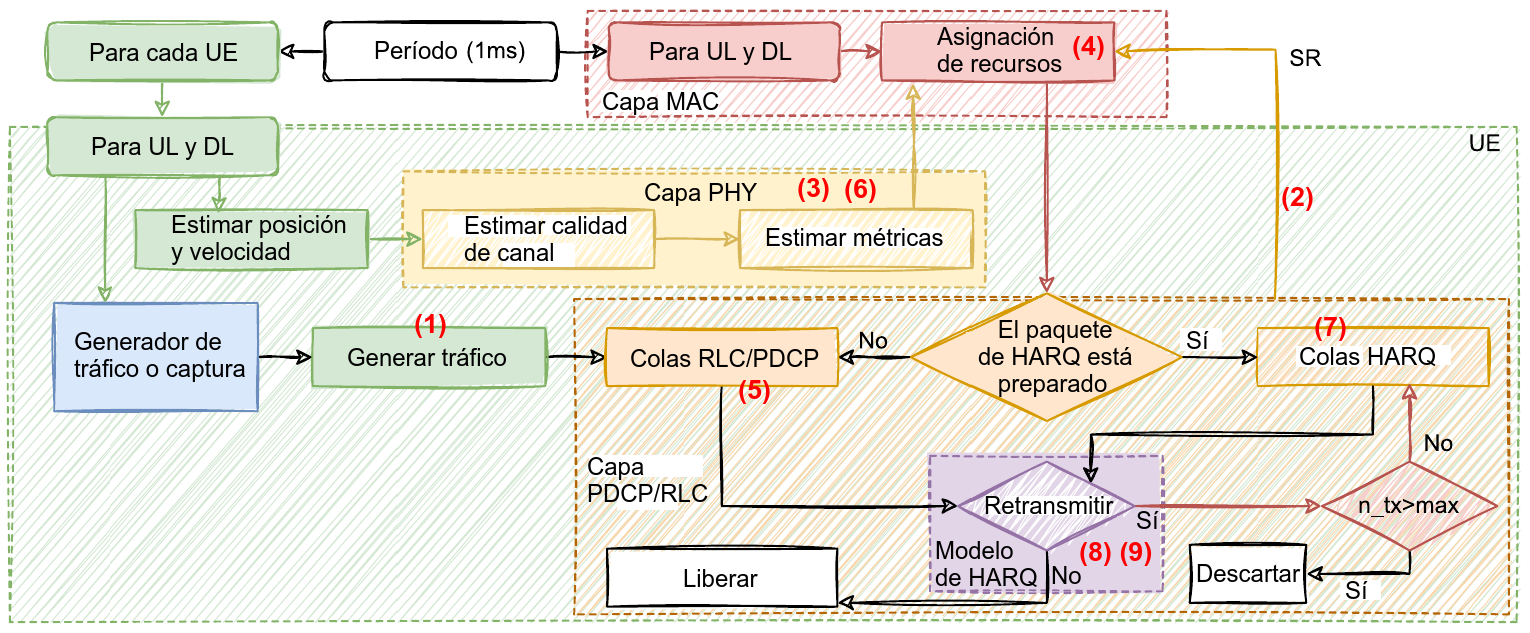
\includegraphics[height=5.0cm]{../memoria/imagenes/fikore_paper/fikore_paper2-001_es_pasos.png}
\end{center}
\end{frame}

%% Diapositiva
%\begin{frame}
%\frametitle{Emulador \textit{FikoRE} - Características generales - Capacidades}
%
%\begin{itemize}
%\item NR (PHY, MAC, PDCP/RLC).
%\item {
%	Red:
%	\begin{itemize}
%	\item Conexión UE a BS (una celda).
%	\item No interacción con otras celdas.
%	\item No comunicación con el núcleo de red.
%	\end{itemize}
%	
%	\begin{center}
%	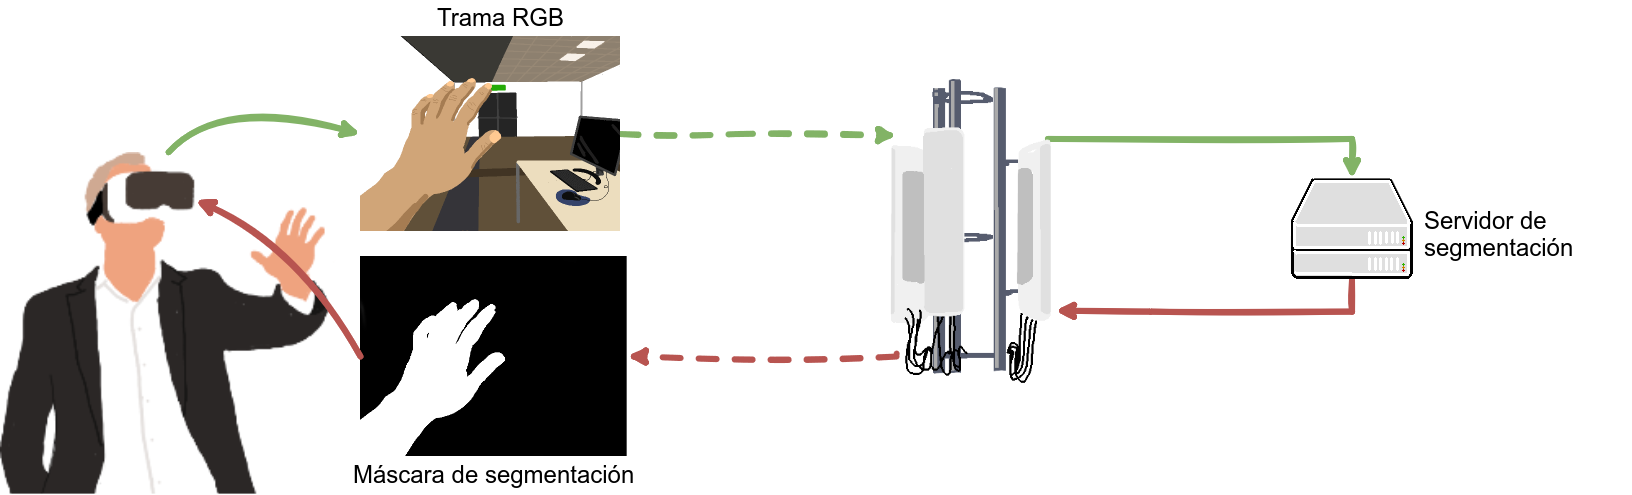
\includegraphics[height=3.0cm]{../memoria/imagenes/fikore_doc/figures/XROffloadingExample_es.png}
%
%	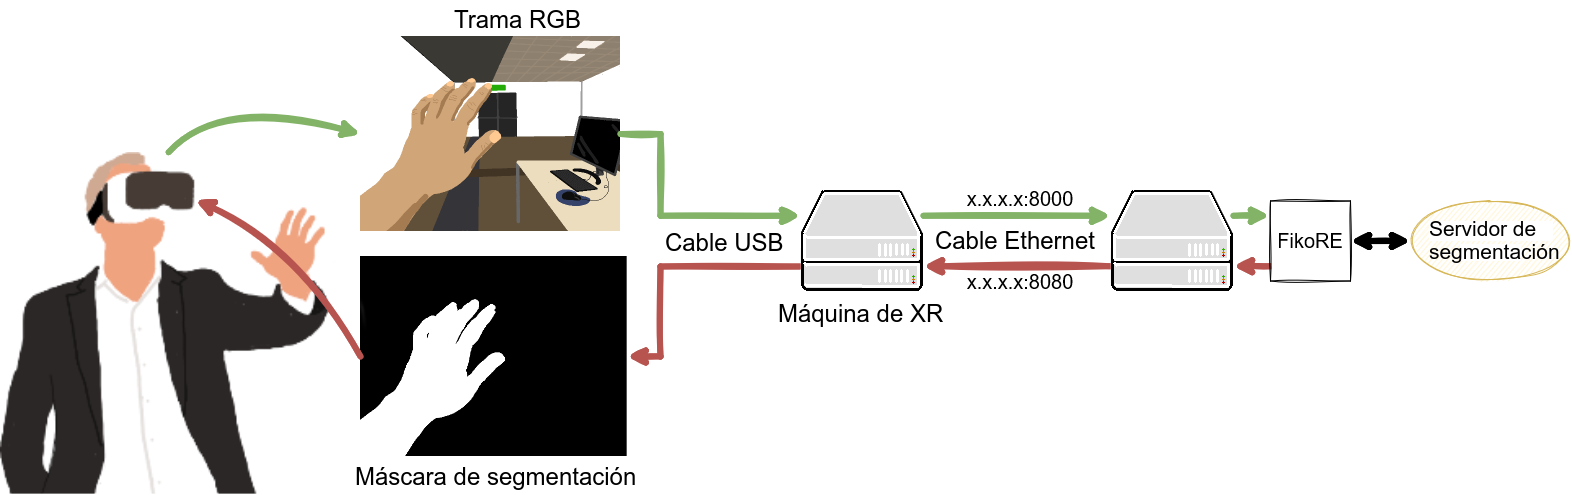
\includegraphics[height=3.0cm]{../memoria/imagenes/fikore_doc/figures/XROffloadingSetup_es.png}
%
%	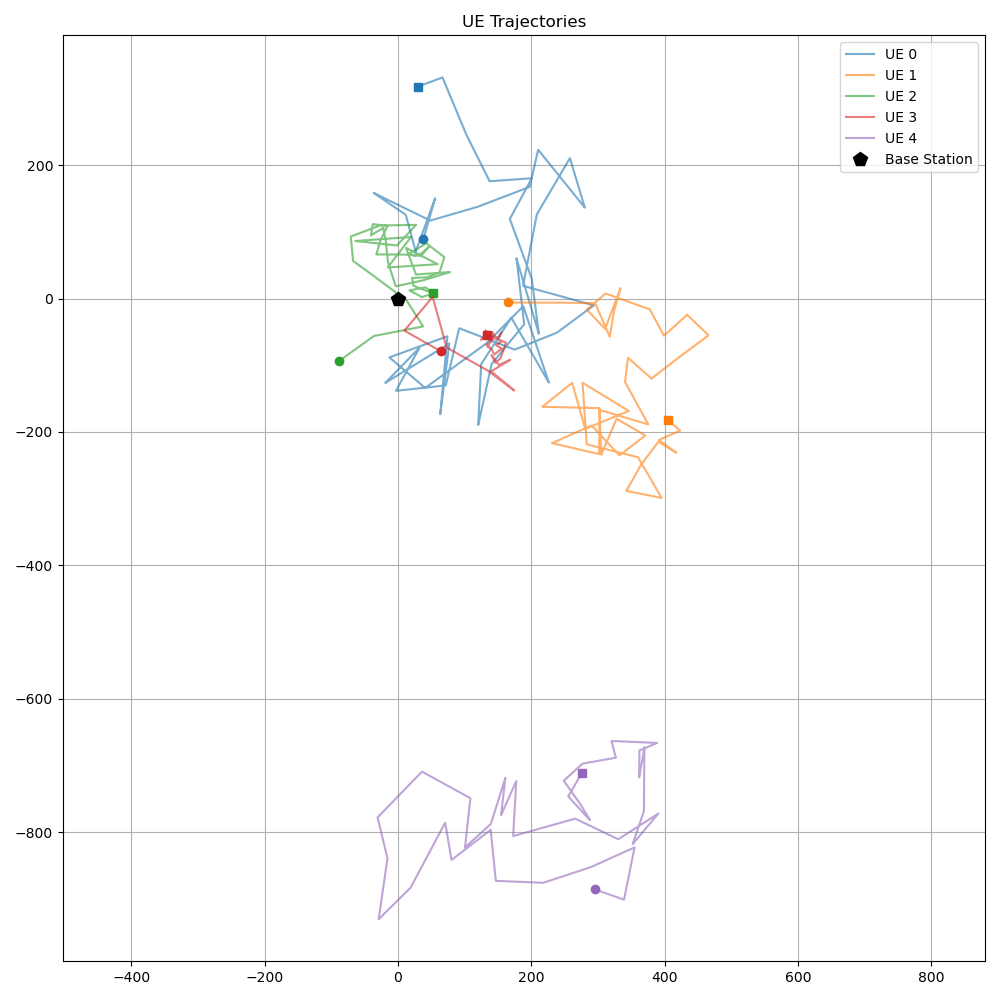
\includegraphics[height=3.0cm]{../computos_y_graficas/pruebas/2_28_19_1_40/ue/trajectory.png}
%	\end{center}
%}
%\item {
%	Interfaz de radio:
%	\begin{itemize}
%	\item Fenómenos de la transmisión inalámbrica:
%	ruido, interferencia, atenuación, desvanecimiento lento, desvanecimiento rápido.
%	\item Sistema celular:
%	interferencia producida por otras células.
%	\item Procesado de señal:
%	modulación OFDM, técnicas multiantena.
%	\item Otras técnicas avanzadas:
%	HARQ, planificación de paquetes, adaptación de enlace, agregación de portadoras.
%	\end{itemize}
%}
%\end{itemize}
%\end{frame}

% Diapositiva
\begin{frame}
\frametitle{Emulador \textit{FikoRE} - Características generales - Capacidades (I)}

\begin{itemize}
\item NR (PHY, MAC, PDCP/RLC).
\item {
	Red:
	\begin{itemize}
	\item Conexión UE a BS (una celda).
	\item No interacción con otras celdas.
	\item No comunicación con el núcleo de red.
	\end{itemize}
	
	\begin{center}
	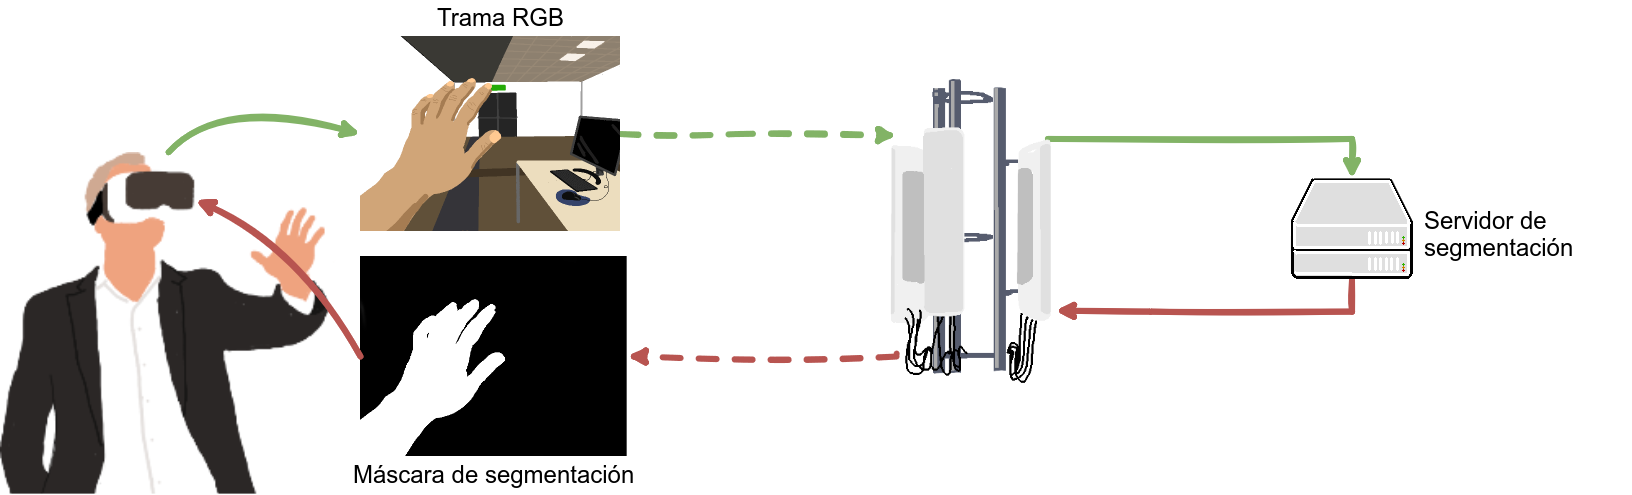
\includegraphics[height=2.5cm]{../memoria/imagenes/fikore_doc/figures/XROffloadingExample_es.png}

	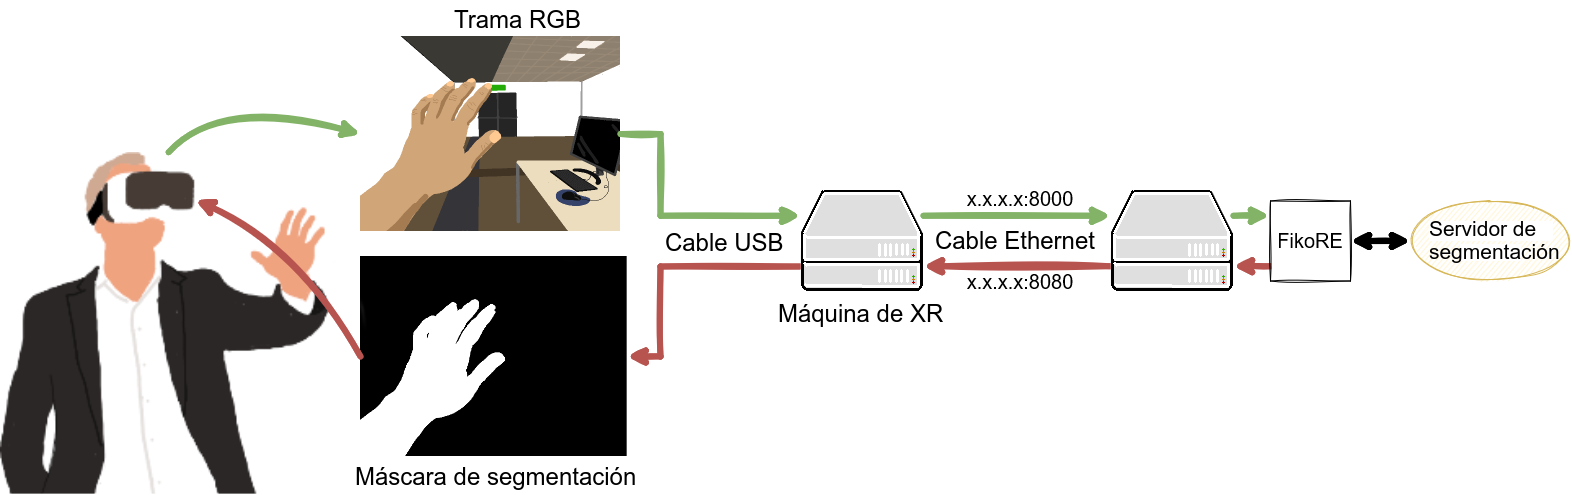
\includegraphics[height=2.5cm]{../memoria/imagenes/fikore_doc/figures/XROffloadingSetup_es.png}
	\end{center}
}
\end{itemize}
\end{frame}

% Diapositiva
\begin{frame}
\frametitle{Emulador \textit{FikoRE} - Características generales - Capacidades (II)}

\begin{itemize}
\item {
	Red:
	\begin{center}
	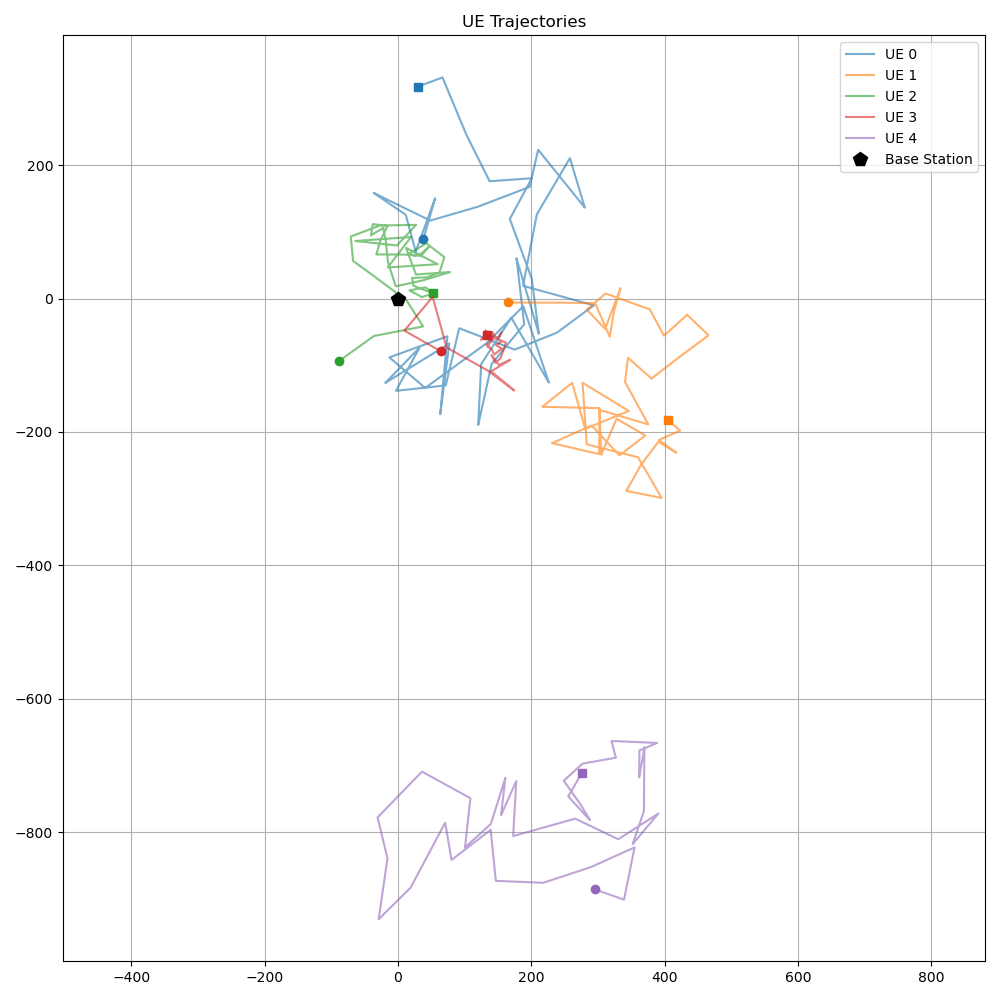
\includegraphics[height=7.0cm]{../computos_y_graficas/pruebas/2_28_19_1_40/ue/trajectory.png}
	\end{center}
}
\end{itemize}
\end{frame}

% Diapositiva
\begin{frame}
\frametitle{Emulador \textit{FikoRE} - Características generales - Capacidades (III)}

\begin{itemize}
\item {
	Interfaz de radio:
	\begin{itemize}
	\item Fenómenos de la transmisión inalámbrica:
	ruido, interferencia, atenuación, desvanecimiento lento, desvanecimiento rápido.
	\item Sistema celular:
	interferencia producida por otras células.
	\item Procesado de señal:
	modulación OFDM, técnicas multiantena.
	\item Otras técnicas avanzadas:
	HARQ, planificación de paquetes, adaptación de enlace, agregación de portadoras.
	\end{itemize}
}
\end{itemize}
\end{frame}

\subsection{Detalles particulares}

% Diapositiva
\begin{frame}
\frametitle{Emulador \textit{FikoRE} - Detalles particulares - Validación del funcionamiento}

\begin{itemize}
\item {
	Varios experimentos en las fuentes:
	\begin{itemize}
	\item UE era estático.
	\item Línea de visión.
	\end{itemize}
}
\item Es necesario validar comportamientos.
\end{itemize}
\end{frame}

%% Diapositiva
%\begin{frame}
%\frametitle{Emulador \textit{FikoRE} - Detalles particulares - Relativas a la ejecución}
%
%\begin{itemize}
%\item {
%	Duplicidad de instancias (UL/DL).
%	\begin{center}
%	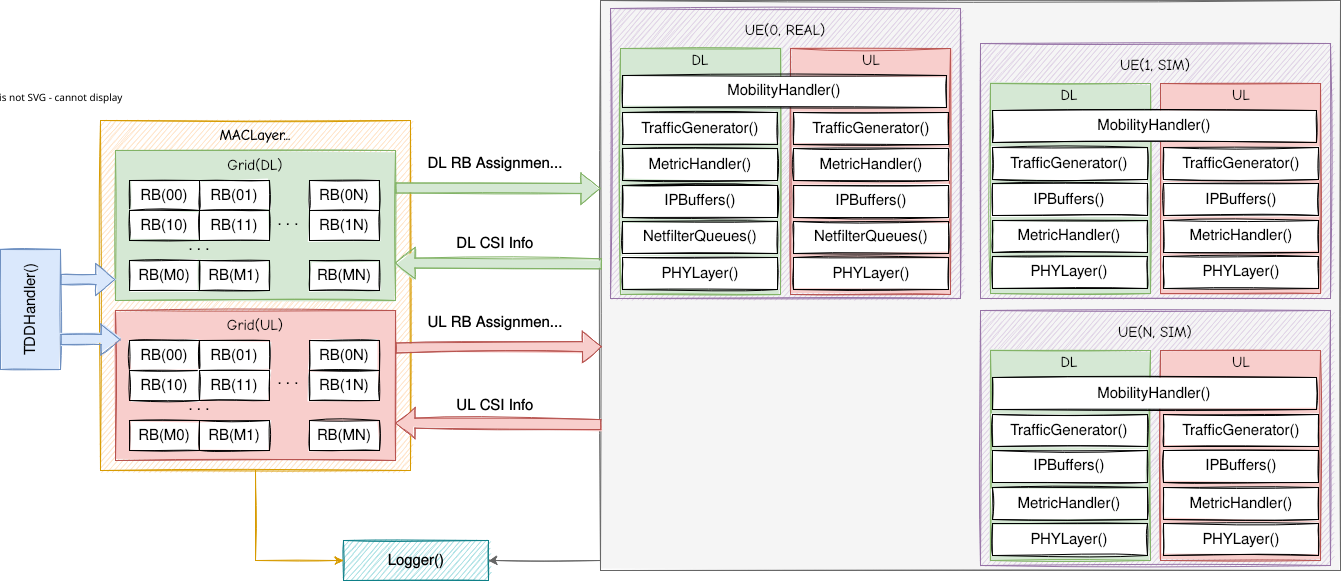
\includegraphics[height=5.0cm]{../memoria/imagenes/fikore_doc/figures/EmuImplementation.png}
%	\end{center}
%}
%\item {
%	Sincronía de la ejecución.
%	\begin{itemize}
%	\item Período de ejecución (1 ms por defecto).
%	\item UE y capa MAC (gNB) consecutivamente.
%	\end{itemize}
%}
%\item {
%	Módulo \textit{Netfilter Queue}.
%	\begin{itemize}
%	\item API del espacio de usuario de \textit{Linux}.
%	\item Acceder a los paquetes que han sito encolados por el cortafuegos (\textit{firewall}).
%	\end{itemize}
%}
%\end{itemize}
%\end{frame}

% Diapositiva
\begin{frame}
\frametitle{Emulador \textit{FikoRE} - Detalles particulares - Relativas a la ejecución (I)}

\begin{itemize}
\item {
	Duplicidad de instancias (UL/DL).
	\begin{center}
	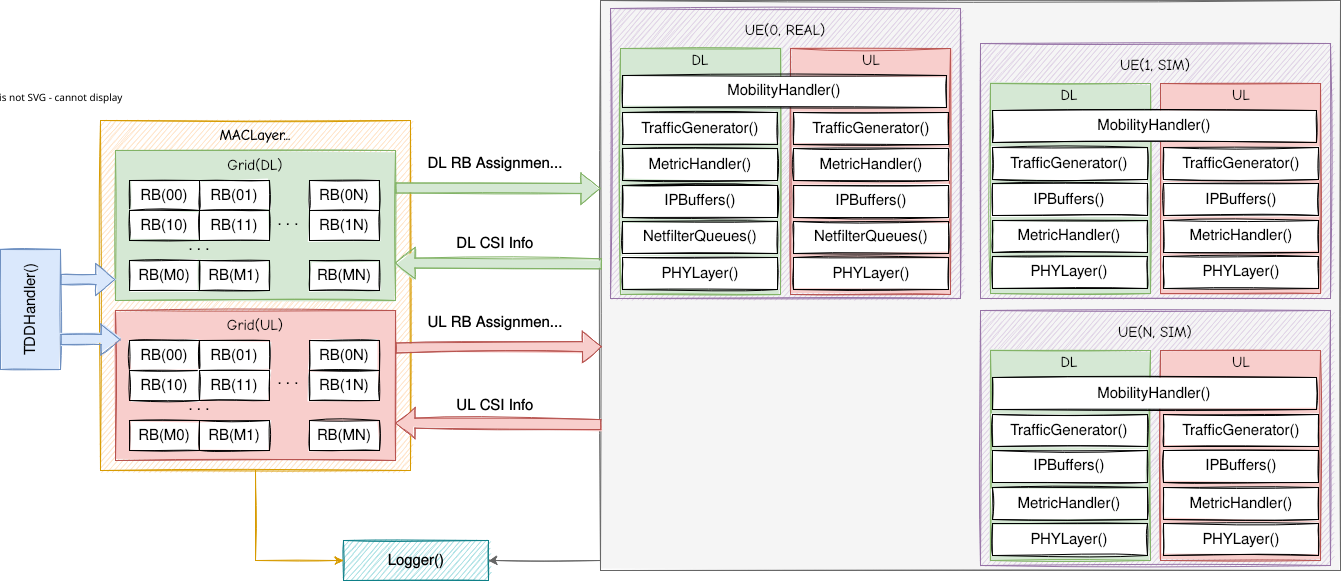
\includegraphics[height=4.5cm]{../memoria/imagenes/fikore_doc/figures/EmuImplementation.png}
	\end{center}
}
\end{itemize}
\end{frame}

% Diapositiva
\begin{frame}
\frametitle{Emulador \textit{FikoRE} - Detalles particulares - Relativas a la ejecución (II)}

\begin{itemize}
\item {
	Sincronía de la ejecución.
	\begin{itemize}
	\item Período de ejecución (1 ms por defecto).
	\item UE y capa MAC (gNB) consecutivamente.
	\end{itemize}
}
\item {
	Módulo \textit{Netfilter Queue}.
	\begin{itemize}
	\item API del espacio de usuario de \textit{Linux}.
	\item Acceder a los paquetes que han sito encolados por el cortafuegos (\textit{firewall}).
	\end{itemize}
}
\end{itemize}
\end{frame}

%% Diapositiva
%\begin{frame}
%\frametitle{Emulador \textit{FikoRE} - Detalles particulares - Asunciones en la simulación}
%
%\begin{itemize}
%\item {
%	Tasa de asignación de recursos de radio
%	\begin{itemize}
%	\item RRM una vez por período, no por \textit{slot}. $\rightarrow$ Reduce la exactitud cuando el UE se desplace a gran velocidad.
%	\end{itemize}
%}
%\item {
%	Ruido e interferencia
%	\begin{itemize}
%	\item UE estima el ruido y la interferencia al comienzo de una simulación. $\rightarrow$ Anula la varianza.
%	\end{itemize}
%}
%\item {
%	Velocidad máxima en \textit{Uma}
%	\begin{itemize}
%	\item \textasciitilde 0.8 m/s $\rightarrow$ No es posible simular UE a gran velocidad en un entorno urbano.
%	\end{itemize}
%}
%\item {
%	Modelos de canal
%	\begin{itemize}
%	\item {
%		Especificación 3GPP 38.901.
%		
%		\begin{center}
%		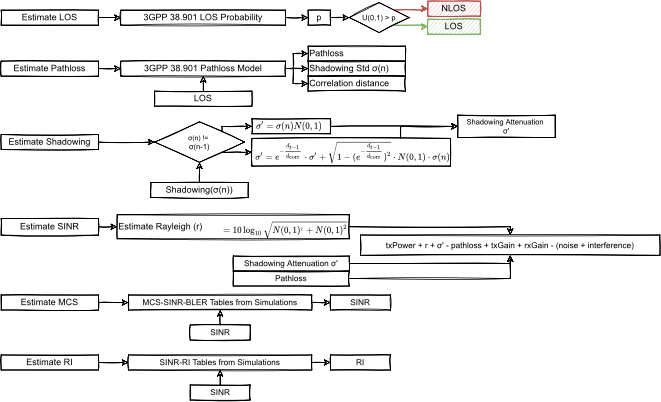
\includegraphics[height=5.0cm]{../memoria/imagenes/fikore_doc/figures/ModelsPHY.png}
%		\end{center}
%	}
%	\item {
%		Forma:
%		\begin{itemize}
%		\item diversos efectos: atenuación, desvanecimiento lento, desvanecimiento rápido
%		\item forma estadística
%		\item variables de entrada (distancia del UE a la gNB, anchura de la calle, altura de la gNB, etc.)
%		\item estimación de los parámetros que afectarán a la calidad de la transmisión (SINR, latencia, etc.)
%		\end{itemize}
%		
%		\begin{center}
%			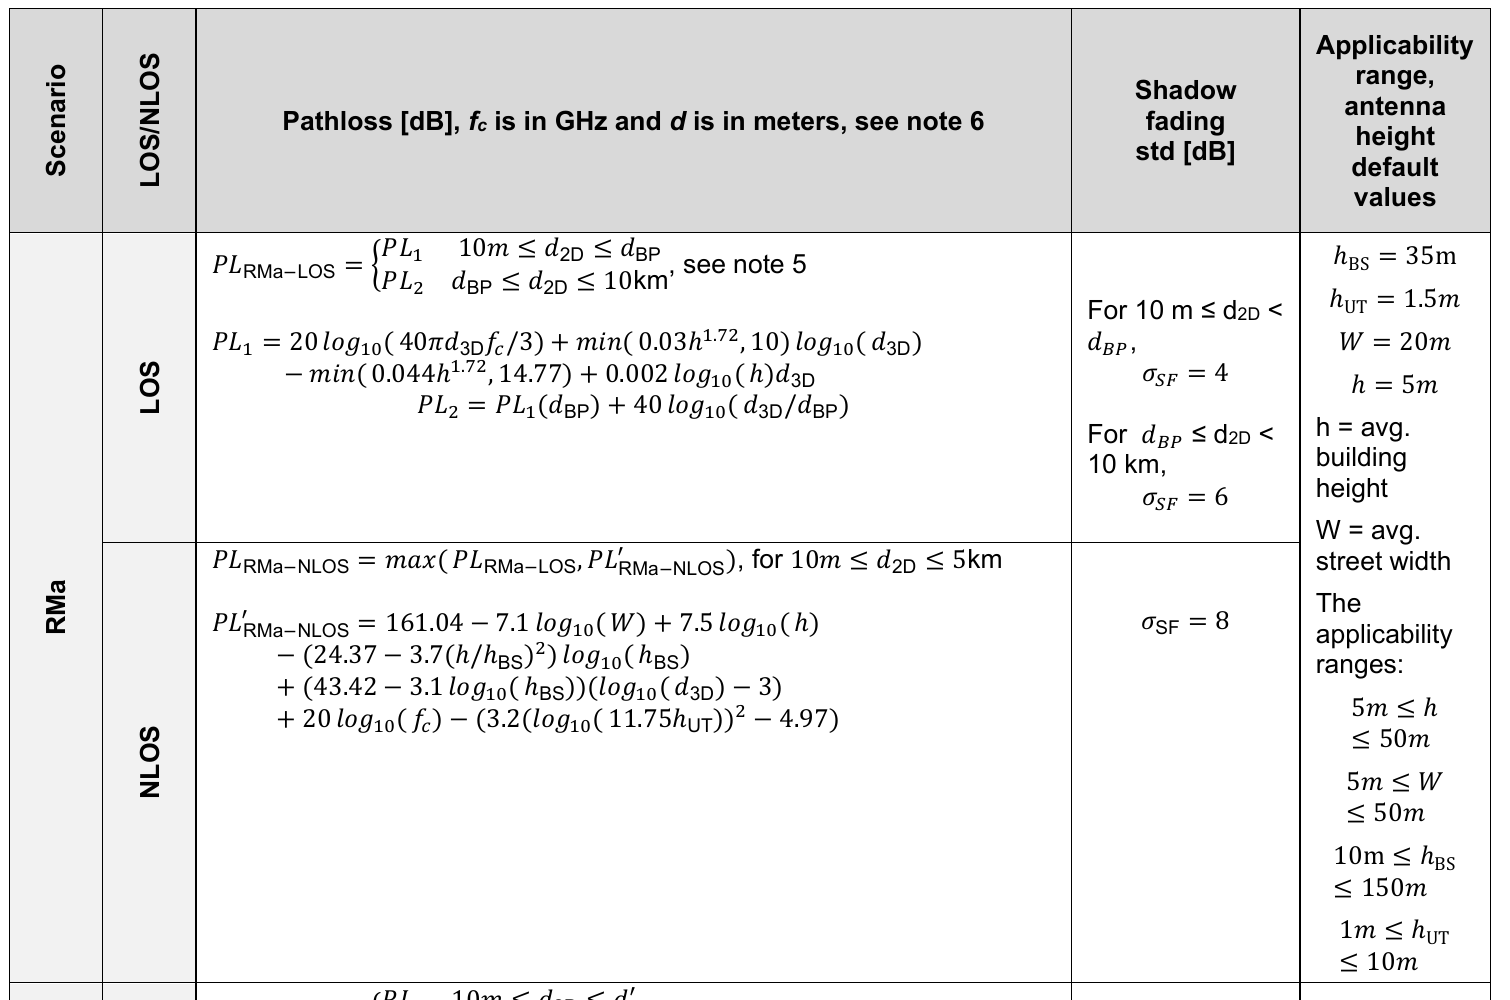
\includegraphics[height=5.0cm]{../memoria/imagenes/3gpp_ts_38901/TS_38901_extracto_1.png}
%		
%			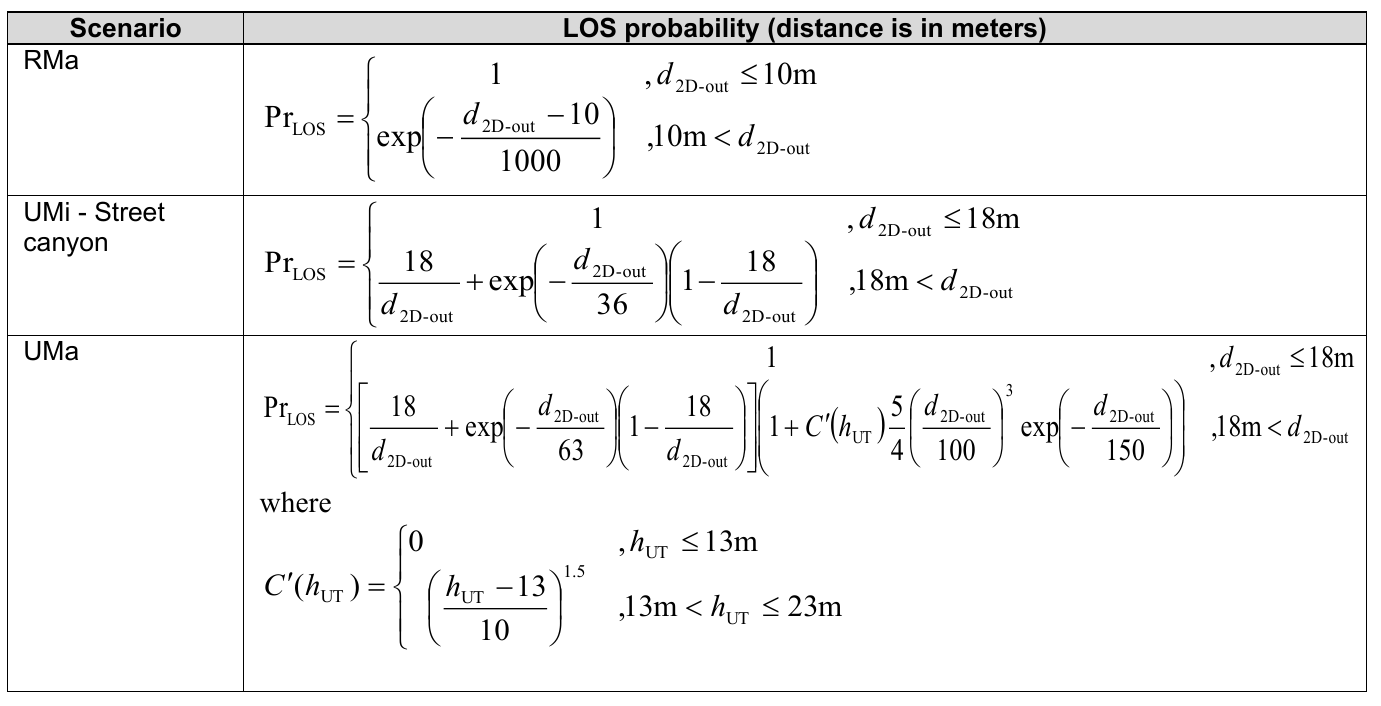
\includegraphics[height=5.0cm]{../memoria/imagenes/3gpp_ts_38901/TS_38901_extracto_2.png}
%		\end{center}
%	}
%	\item {
%		Calidad:
%		\begin{itemize}
%		\item Otros modelos: \textit{IEEE}, \textit{COST}, \textit{Nokia}, \textit{Ericsson}, \textit{Huawei}, etc.
%		\item Precisión necesaria para 5G $<$ \textit{FikoRE} $<$ despliegue real profesional.
%		\end{itemize}
%	}
%	\end{itemize}
%}
%\item {
%	Efecto Doppler:
%	\begin{itemize}
%	\item {
%		Importancia:
%		\begin{itemize}
%		\item Fenómeno determinante en cuando el UE se desplaza a gran velocidad en entornos urbanos.
%		\item Se relaciona con el multitrayecto (canal variante en el tiempo y la frecuencia).
%		\end{itemize}
%	}
%	\item {
%		Código:
%		\begin{itemize}
%		\item Variables: \textit{doppler\_f}, \textit{tc}, \textit{min\_sinr\_update}, \textit{sinr\_period}, \textit{update\_sinr}.
%		\item Métodos: \textit{init\_update\_rates()}, \textit{estimate\_channel\_state()}.
%		\end{itemize}
%	}
%	\item {
%		\begin{center}
%		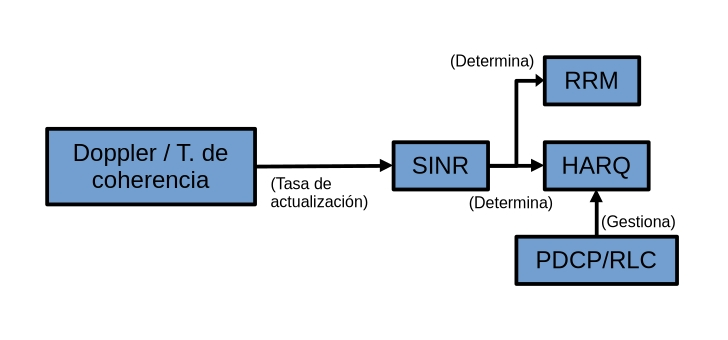
\includegraphics[height=5.0cm]{../memoria/imagenes/elaboracion_propia/ep_esquema_del_emulador.jpg}
%		
%		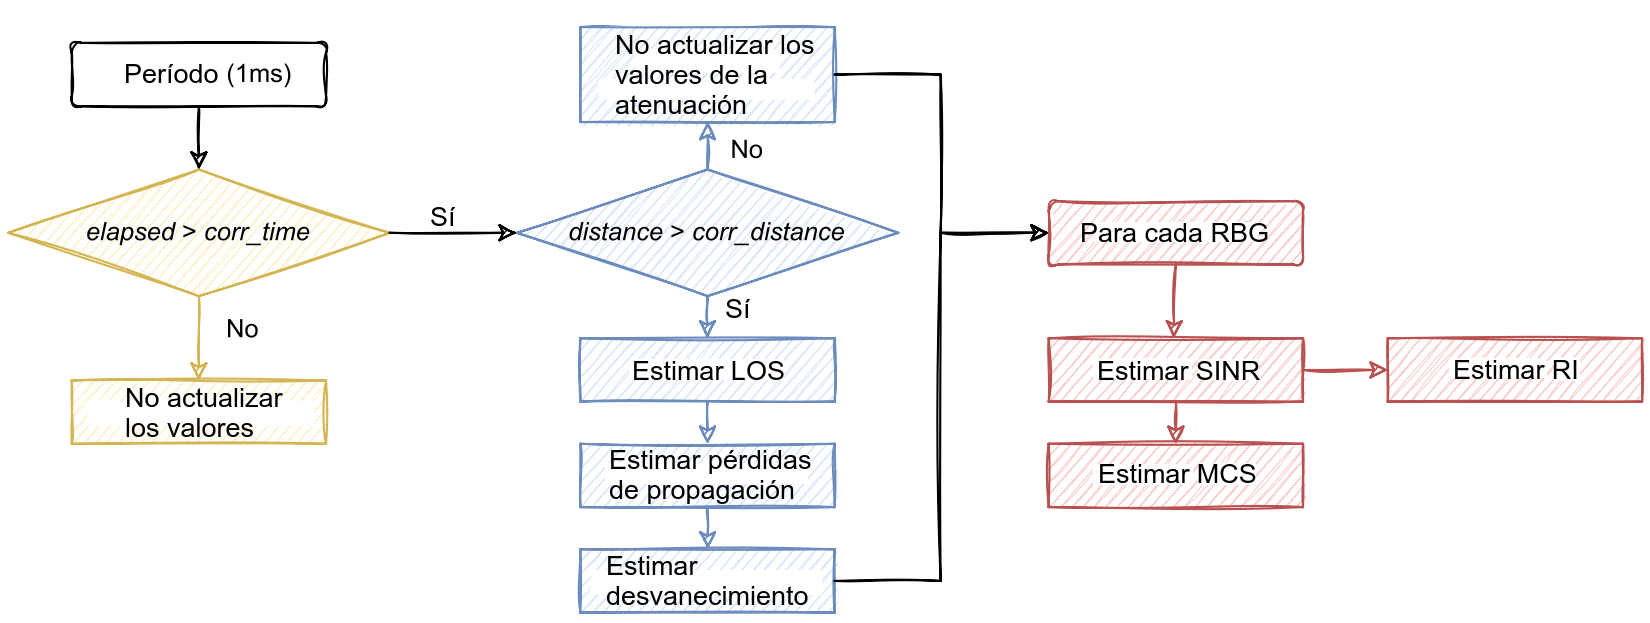
\includegraphics[height=5.0cm]{../memoria/imagenes/fikore_doc/figures/PHYFlow_es.png}
%		\end{center}
%	}
%	\item {
%		Simulaciones:
%		\begin{itemize}
%		\item \textit{Validación - Efecto Doppler (conjunto 1)}
%		\item \textit{Validación - Efecto Doppler (conjunto 2)}
%		\item \textit{Validación - Efecto Doppler (conjunto 3)}
%		\item \textit{Validación - Efecto Doppler (conjunto 4)}
%		\item \textit{Validación - Efecto Doppler (conjunto 5)}
%		\end{itemize}
%	}
%	\item UE que se alejaba de la gNB a la misma velocidad.
%	\item Velocidad creciente.
%	\item SINR similar.
%	\item Distinta precisión temporal (\textit{period}).
%	\item Distinta tasa de reporte de datos (\textit{log\_freq}).
%	\item Distinta tasa de actualización de parámetros de CQI (\textit{cqi\_period}, \textit{ri\_period}).
%	\item Las velocidades altas no suponen un gran cambio en MCS, tasa binaria, RI, RSRP, SINR o CQI.
%	\item AMC permiten mantener las mismas tasas pese al incremento de velocidad.
%	\item Cambios achacables a peculiaridades estadísticas (tráfico generado, trayectoria seguida, etc.) del único UE simulado.
%	\item {
%		\begin{center}
%		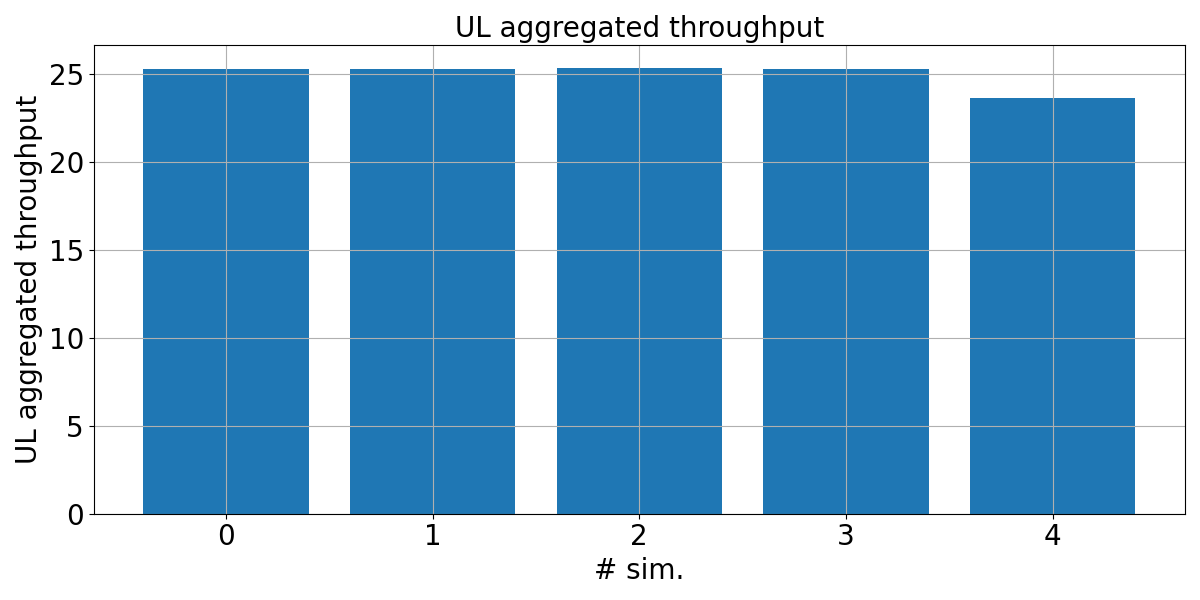
\includegraphics[height=5.0cm]{../comparaciones/validacion_doppler_conjunto2/ue/ul_agg_throughput_multi_sim.png}
%		
%		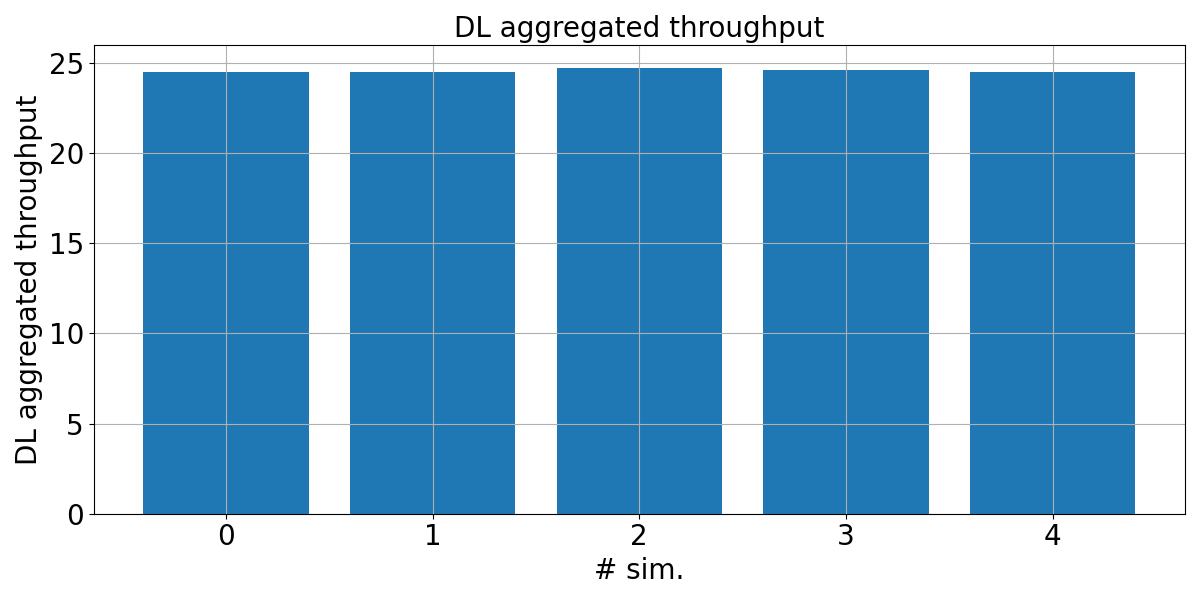
\includegraphics[height=5.0cm]{../comparaciones/validacion_doppler_conjunto2/ue/dl_agg_throughput_multi_sim.png}
%		
%		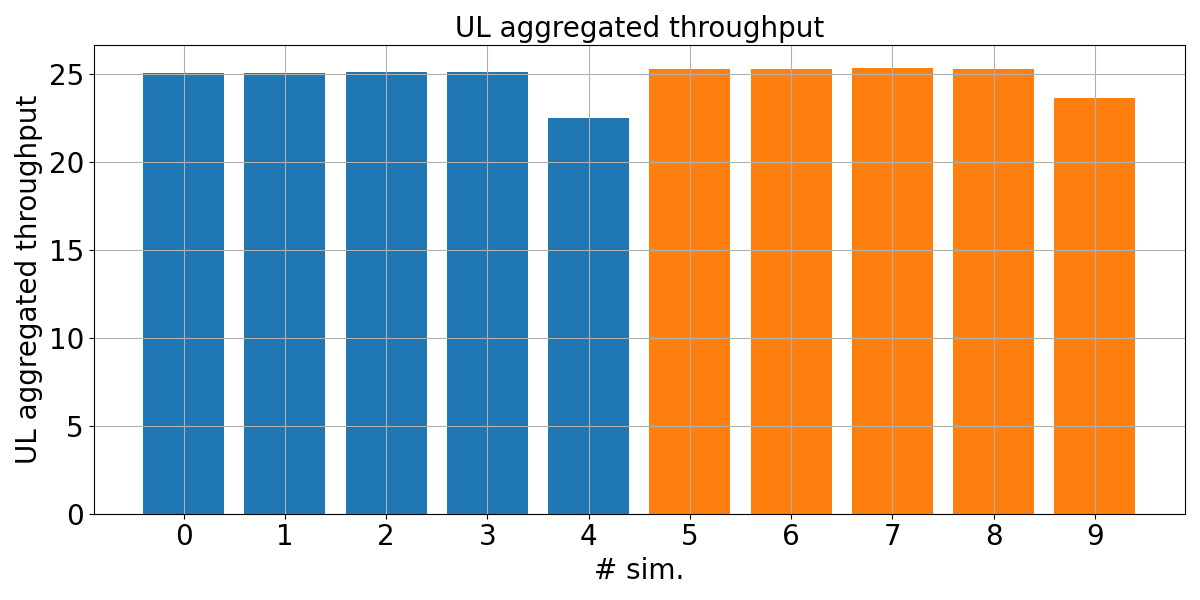
\includegraphics[height=5.0cm]{../comparaciones/validacion_doppler_conjuntos_1_y_2/ue/ul_agg_throughput_multi_sim.png}
%		
%		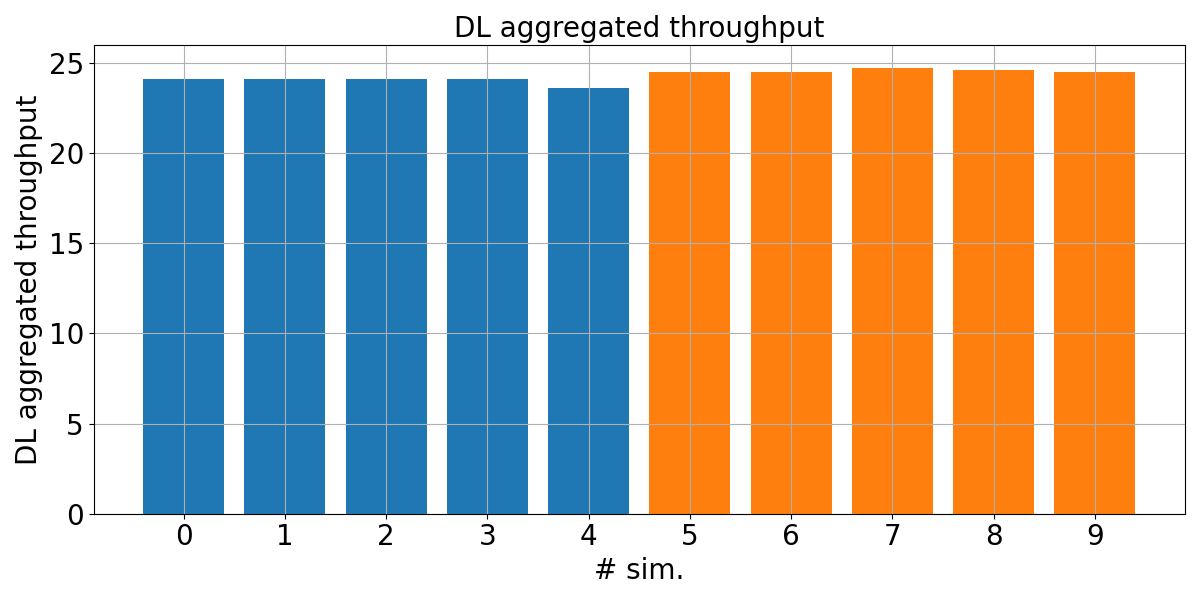
\includegraphics[height=5.0cm]{../comparaciones/validacion_doppler_conjuntos_1_y_2/ue/dl_agg_throughput_multi_sim.png}
%		
%		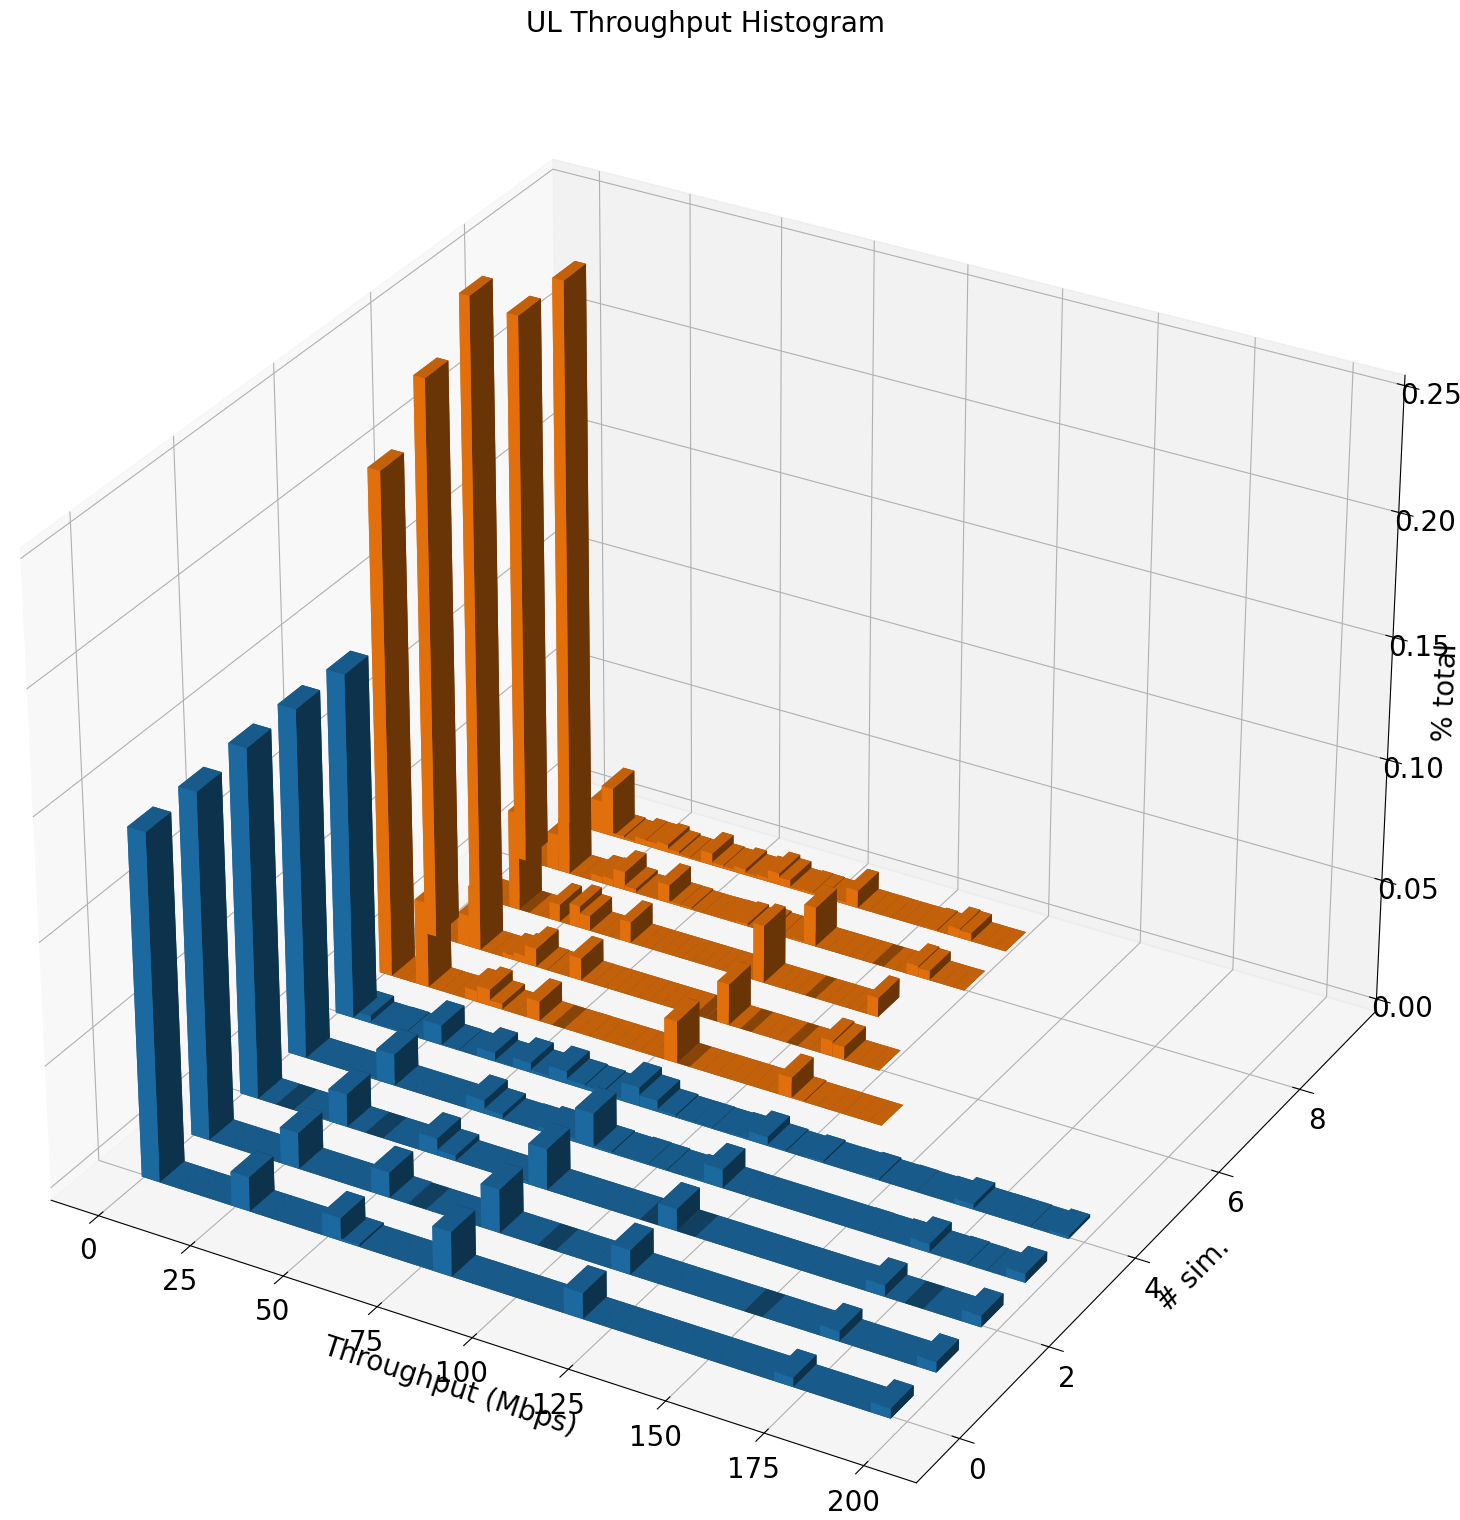
\includegraphics[height=5.0cm]{../comparaciones/validacion_doppler_conjuntos_1_y_2/ue/rul_3d_hist_all_ue_multi.png_cropped.png}
%		
%		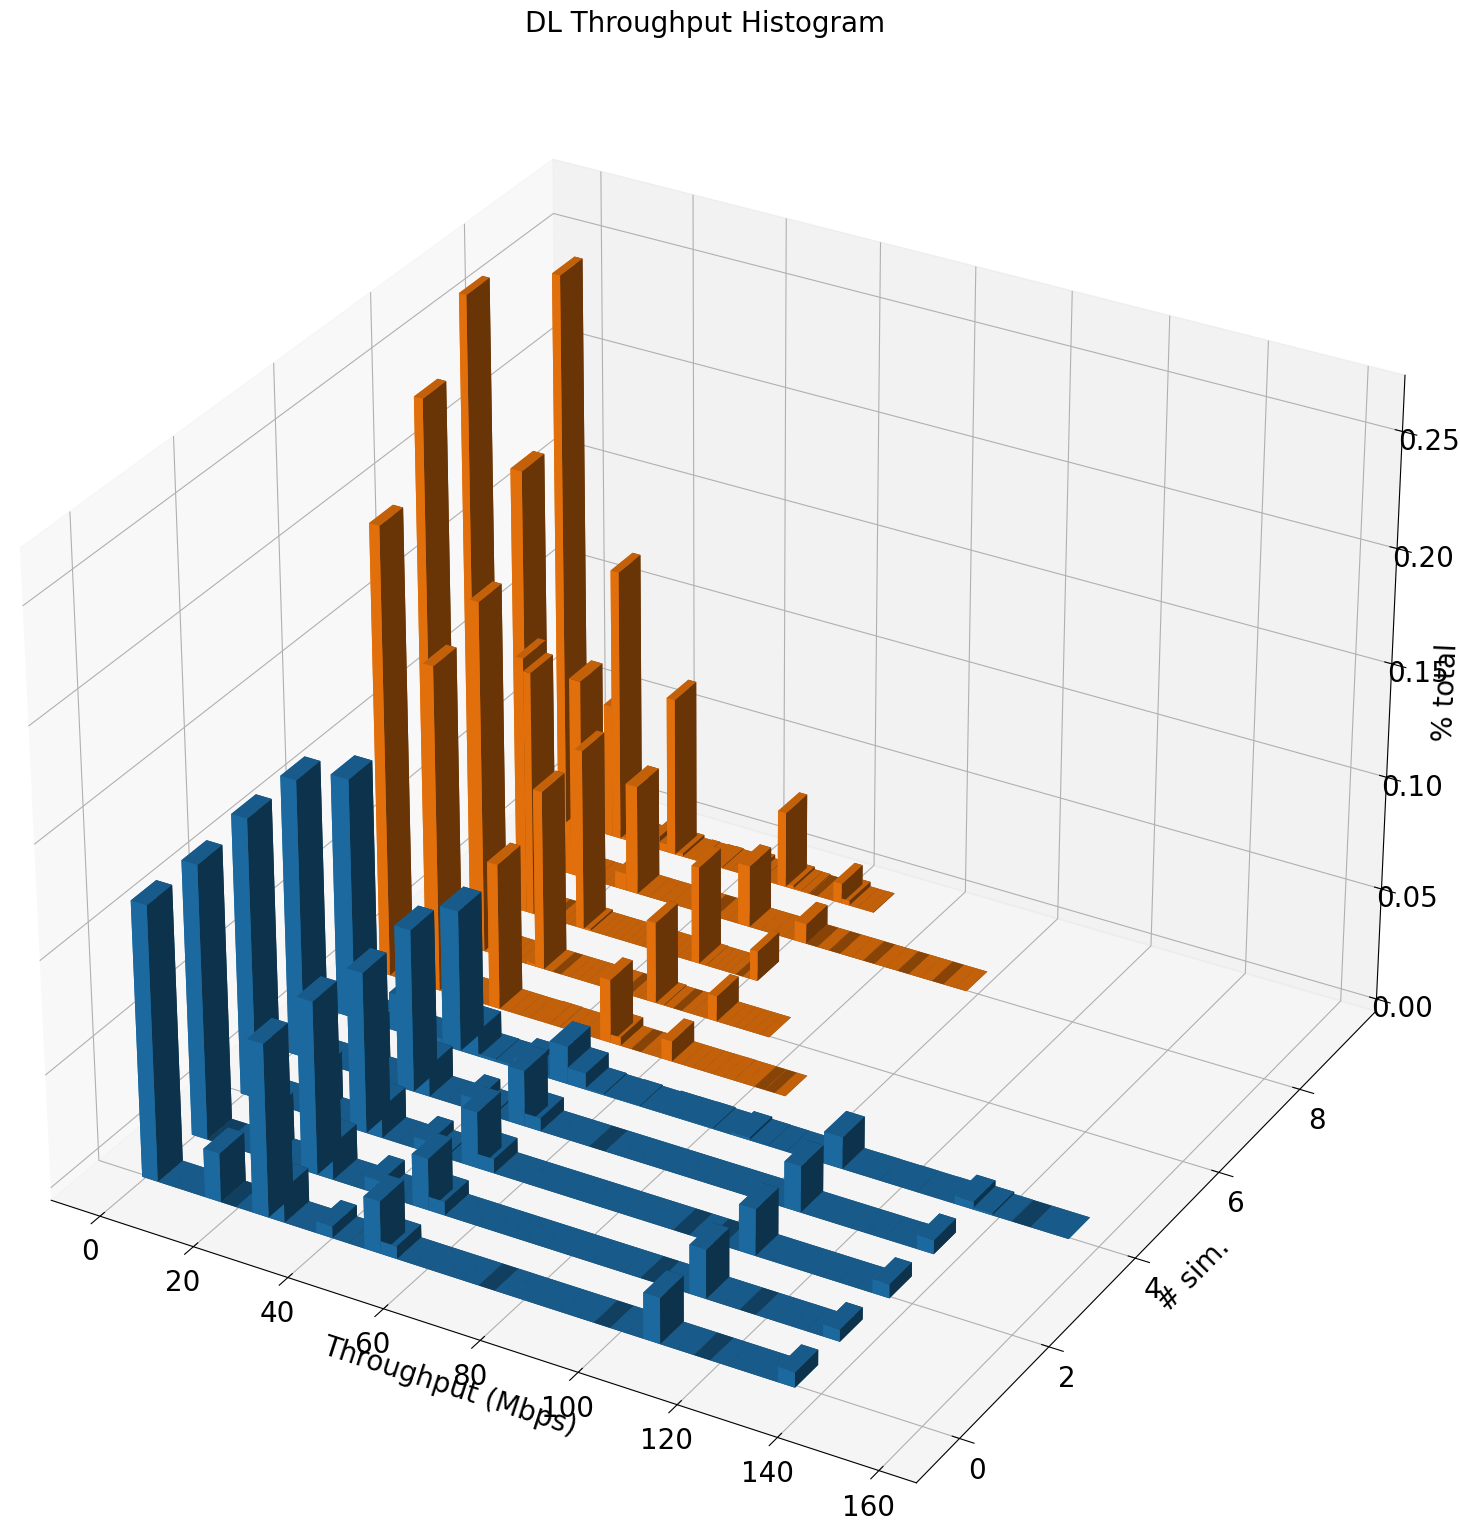
\includegraphics[height=5.0cm]{../comparaciones/validacion_doppler_conjuntos_1_y_2/ue/rdl_3d_hist_all_ue_multi.png_cropped.png}
%		\end{center}
%	}
%	\end{itemize}
%}
%\item {
%	Granularidad temporal
%	\begin{itemize}
%	\item {
%		Simulaciones:
%		\begin{itemize}
%		\item \textit{Validación - Granularidad}
%		\end{itemize}
%	}
%	\item Distinta precisión de la simulación.
%	\item Cálculo de los parámetros posible.
%	\item Distinta tasa binaria
%	\item Mayor tasa, $\rightarrow$ Bloques de menores dimensiones, $\rightarrow$ Evita picos de mayor tasa.
%	\item {
%		\begin{center}
%		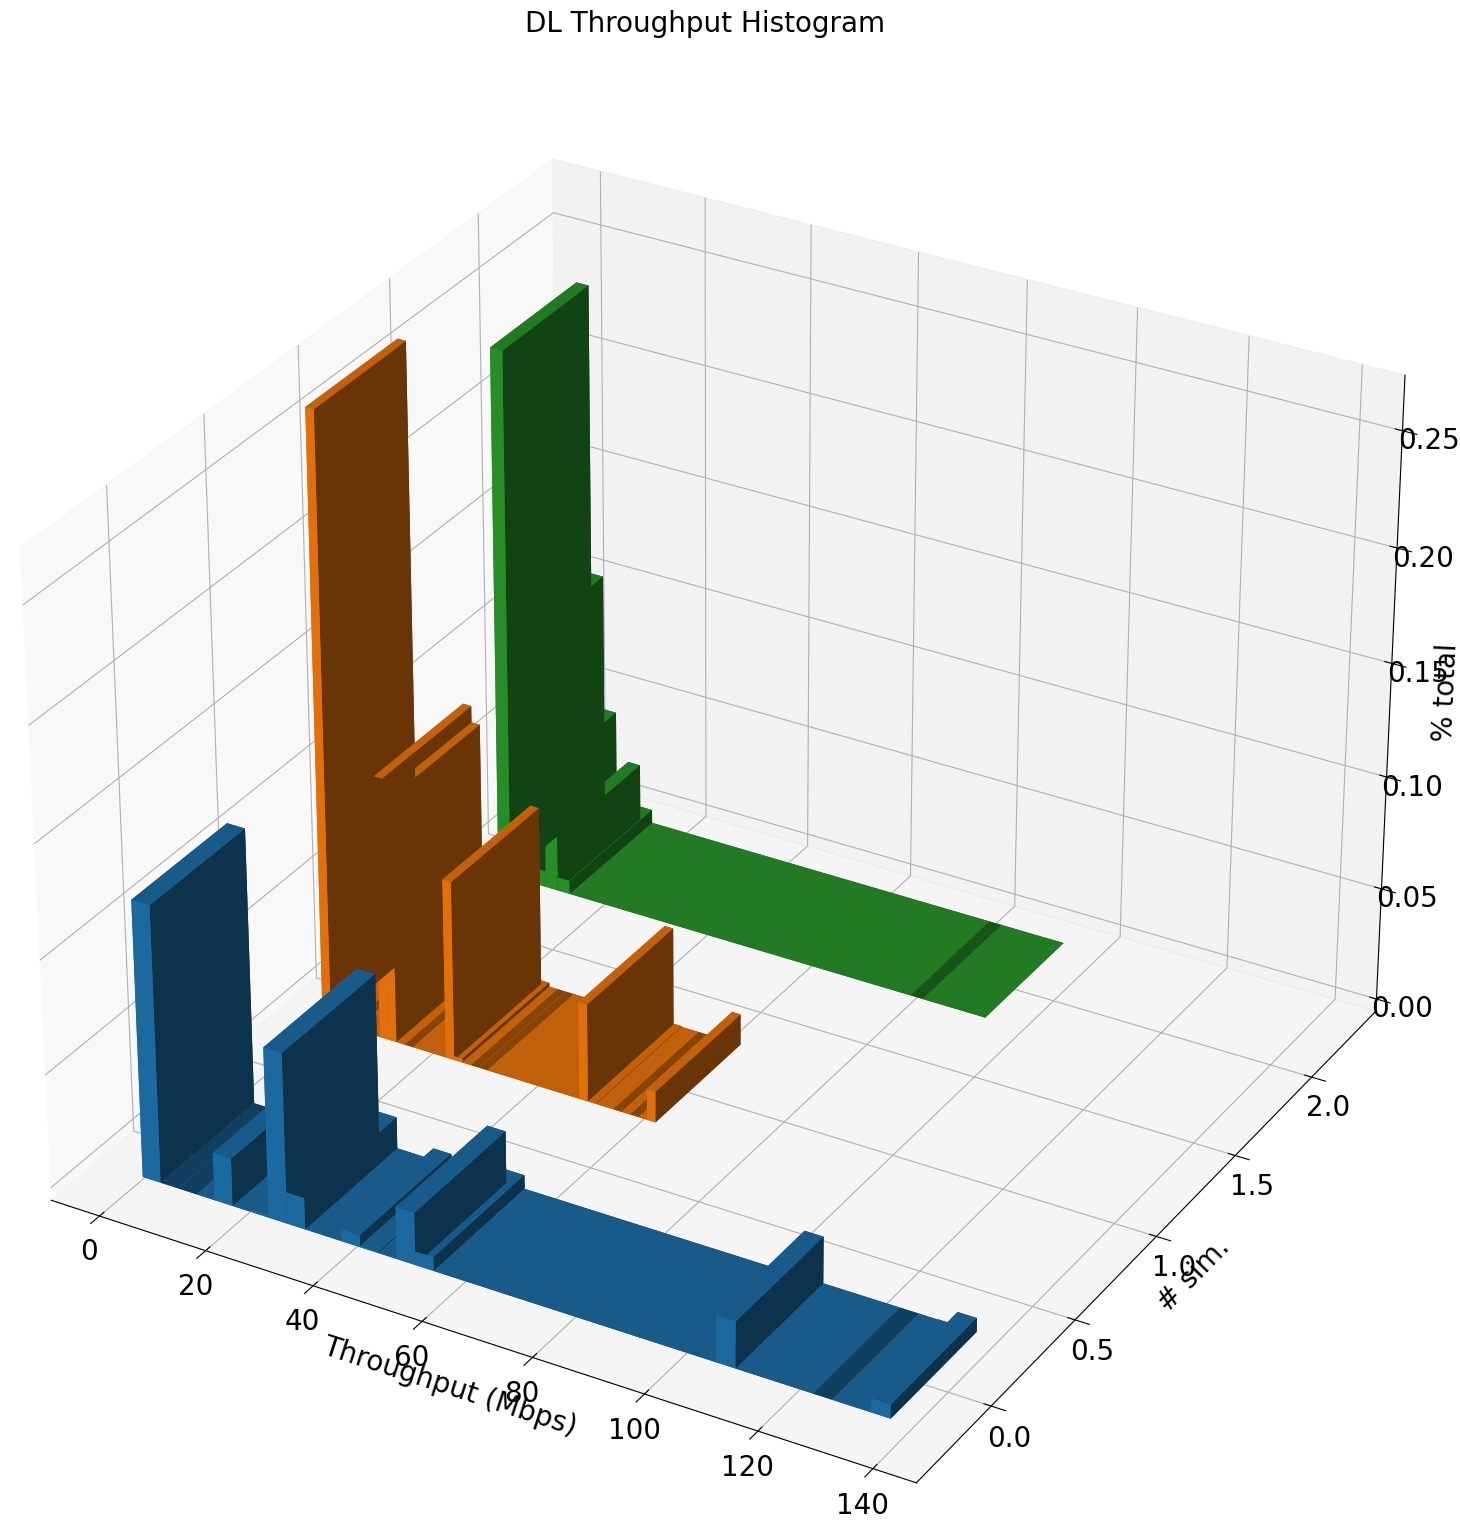
\includegraphics[height=5.0cm]{../comparaciones/validacion_granularidad/ue/rdl_3d_hist_all_ue_multi.png_cropped.png}
%		
%		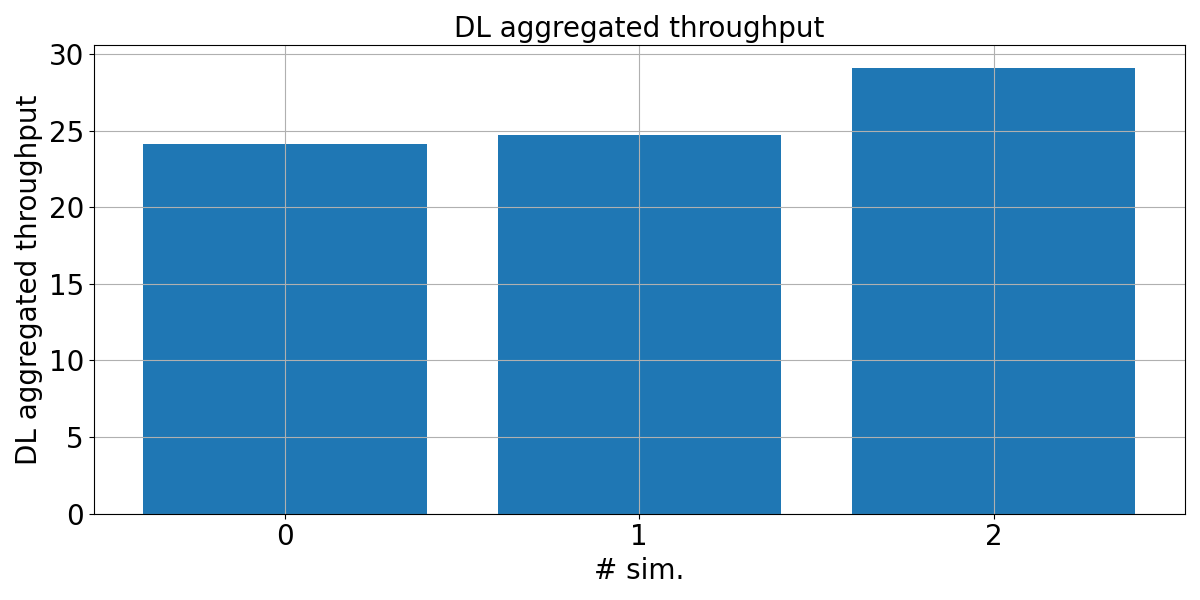
\includegraphics[height=5.0cm]{../comparaciones/validacion_granularidad/ue/dl_agg_throughput_multi_sim.png}
%		\end{center}
%	}
%	\end{itemize}
%}
%\end{itemize}
%\end{frame}

% Diapositiva
\begin{frame}
\frametitle{Emulador \textit{FikoRE} - Detalles particulares - Asunciones en la simulación (I)}

\begin{itemize}
\item {
	Tasa de asignación de recursos de radio
	\begin{itemize}
	\item RRM una vez por período, no por \textit{slot}. $\rightarrow$ Reduce la exactitud cuando el UE se desplace a gran velocidad.
	\end{itemize}
}
\item {
	Ruido e interferencia
	\begin{itemize}
	\item UE estima el ruido y la interferencia al comienzo de una simulación. $\rightarrow$ Anula la varianza.
	\end{itemize}
}
\item {
	Velocidad máxima en \textit{Uma}
	\begin{itemize}
	\item $\textasciitilde 0.8$ m/s $\rightarrow$ No es posible simular UE a gran velocidad en un entorno urbano.
	\end{itemize}
}
\end{itemize}
\end{frame}

% Diapositiva
\begin{frame}
\frametitle{Emulador \textit{FikoRE} - Detalles particulares - Asunciones en la simulación (II)}

\begin{itemize}
\item {
	Modelos de canal
	\begin{itemize}
	\item {
		Especificación 3GPP 38.901.
		
		\begin{center}
		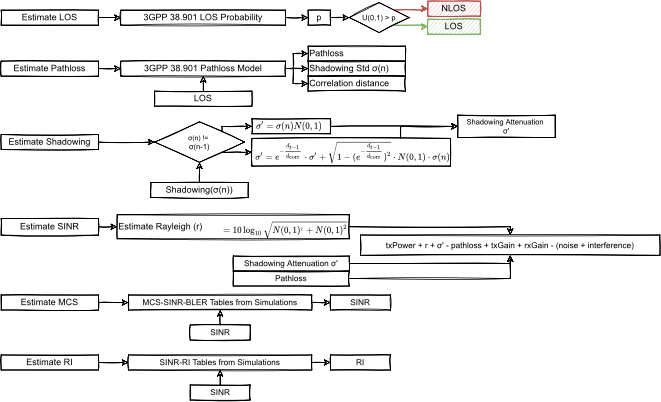
\includegraphics[height=6.0cm]{../memoria/imagenes/fikore_doc/figures/ModelsPHY.png}
		\end{center}
	}
	\end{itemize}
}
\end{itemize}
\end{frame}

% Diapositiva
\begin{frame}
\frametitle{Emulador \textit{FikoRE} - Detalles particulares - Asunciones en la simulación (III)}

\begin{itemize}
\item {
	Modelos de canal
	\begin{itemize}
	\item {
		Forma:
		\begin{itemize}
		\item Diversos efectos: atenuación, desvanecimiento lento, desvanecimiento rápido
		\item Forma estadística
		\item Variables de entrada (distancia del UE a la gNB, anchura de la calle, altura de la gNB, etc.)
		\item Estimación de los parámetros que afectarán a la calidad de la transmisión (SINR, latencia, etc.).
		\end{itemize}
	}
	\end{itemize}
}
\end{itemize}
\end{frame}

% Diapositiva
\begin{frame}
\frametitle{Emulador \textit{FikoRE} - Detalles particulares - Asunciones en la simulación (IV)}

\begin{itemize}
\item {
	Modelos de canal
	\begin{itemize}
	\item {
		Forma:
		\begin{center}
		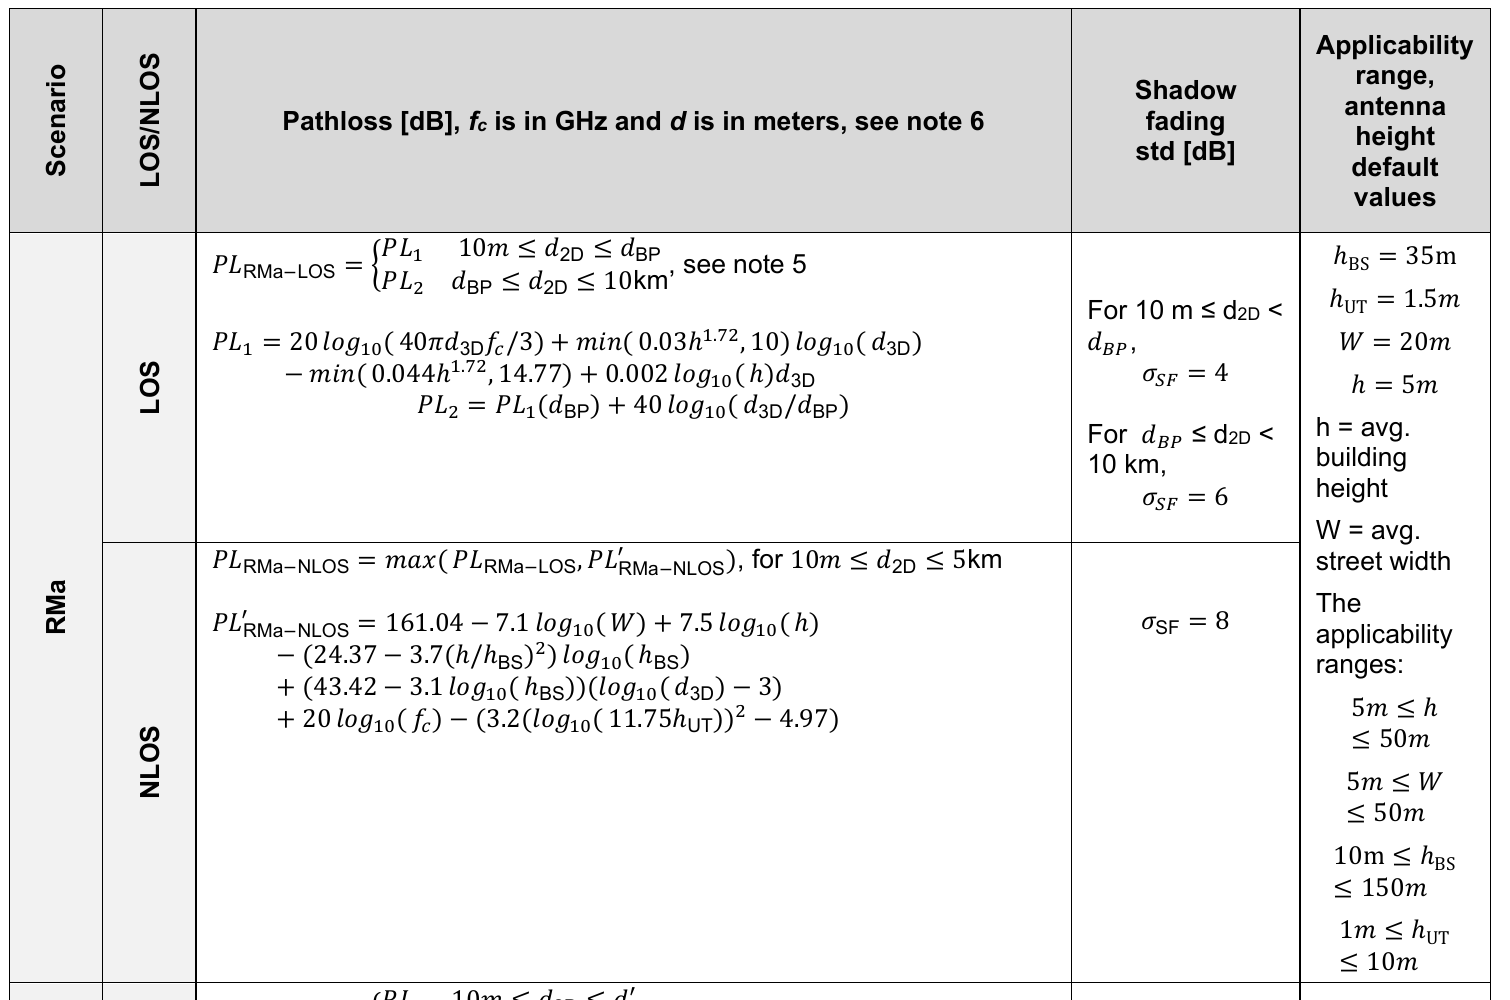
\includegraphics[height=6.0cm]{../memoria/imagenes/3gpp_ts_38901/TS_38901_extracto_1.png}
		\end{center}
	}
	\end{itemize}
}
\end{itemize}
\end{frame}

% Diapositiva
\begin{frame}
\frametitle{Emulador \textit{FikoRE} - Detalles particulares - Asunciones en la simulación (V)}

\begin{itemize}
\item {
	Modelos de canal
	\begin{itemize}
	\item {
		Forma:
		\begin{center}
		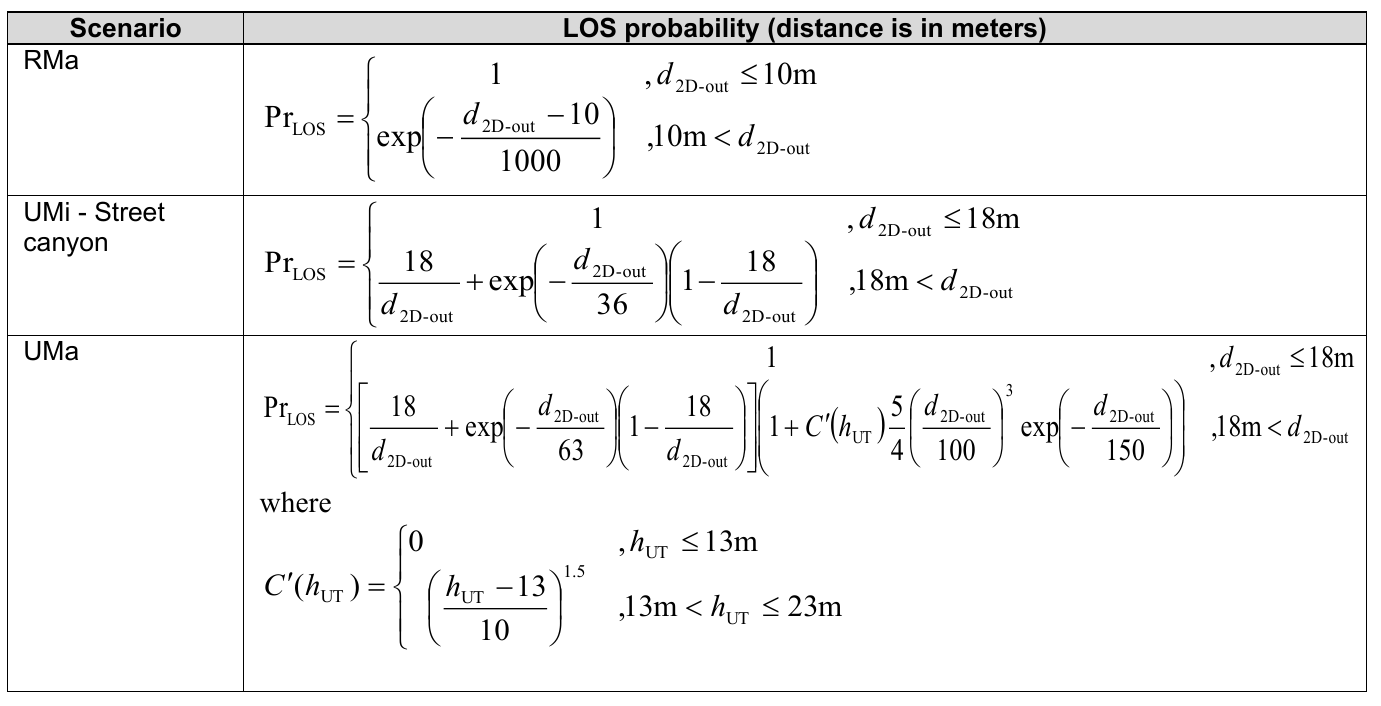
\includegraphics[height=5.0cm]{../memoria/imagenes/3gpp_ts_38901/TS_38901_extracto_2.png}
		\end{center}
	}
	\end{itemize}
}
\end{itemize}
\end{frame}

% Diapositiva
\begin{frame}
\frametitle{Emulador \textit{FikoRE} - Detalles particulares - Asunciones en la simulación (VI)}

\begin{itemize}
\item {
	Modelos de canal
	\begin{itemize}
	\item {
		Calidad:
		\begin{itemize}
		\item Otros modelos: \textit{IEEE}, \textit{COST}, \textit{Nokia}, \textit{Ericsson}, \textit{Huawei}, etc.
		\item Precisión necesaria para 5G $<$ \textit{FikoRE} $<$ despliegue real profesional.
		\end{itemize}
	}
	\end{itemize}
}
\end{itemize}
\end{frame}

% Diapositiva
\begin{frame}
\frametitle{Emulador \textit{FikoRE} - Detalles particulares - Asunciones en la simulación (VII)}

\begin{itemize}
\item {
	Efecto Doppler:
	\begin{itemize}
	\item {
		Importancia:
		\begin{itemize}
		\item Fenómeno determinante en cuando el UE se desplaza a gran velocidad en entornos urbanos.
		\item Se relaciona con el multitrayecto (canal variante en el tiempo y la frecuencia).
		\end{itemize}
	}
	\item {
		Código:
		\begin{itemize}
		\item Variables: \textit{doppler\_f}, \textit{tc}, \textit{min\_sinr\_update}, \textit{sinr\_period}, \textit{update\_sinr}.
		\item Métodos: \textit{init\_update\_rates()}, \textit{estimate\_channel\_state()}.
		\end{itemize}
	}
	\end{itemize}
}
\end{itemize}
\end{frame}

% Diapositiva
\begin{frame}
\frametitle{Emulador \textit{FikoRE} - Detalles particulares - Asunciones en la simulación (VIII)}

\begin{itemize}
\item {
	Efecto Doppler:
	\begin{center}
	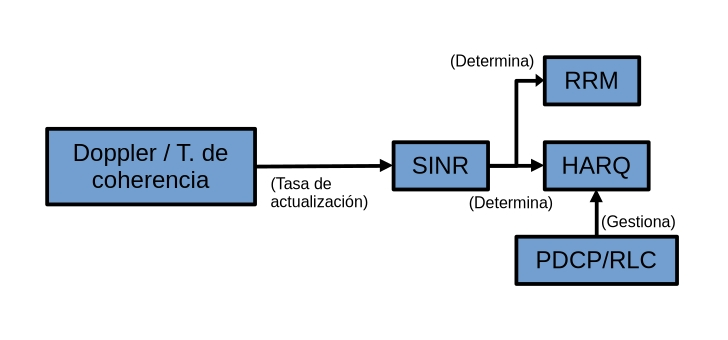
\includegraphics[height=3.0cm]{../memoria/imagenes/elaboracion_propia/ep_esquema_del_emulador.jpg}
	
	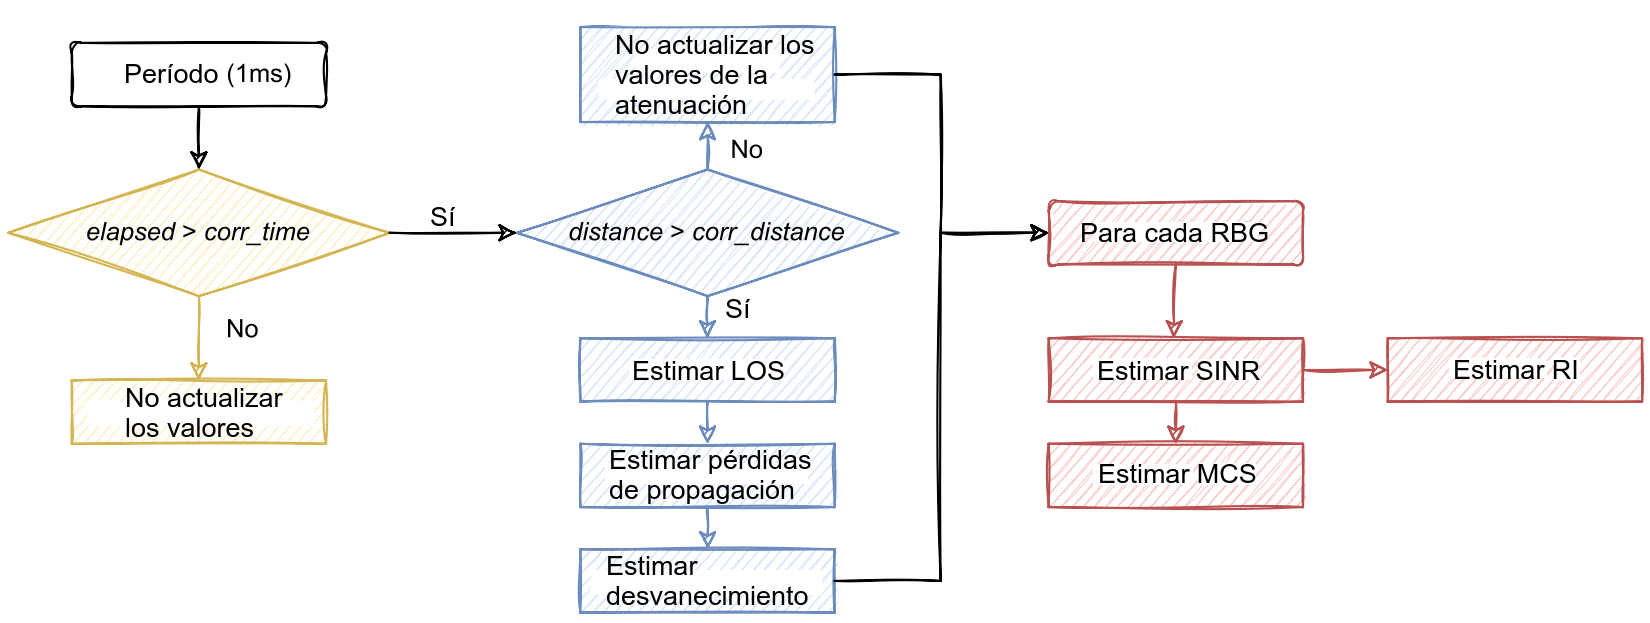
\includegraphics[height=3.5cm]{../memoria/imagenes/fikore_doc/figures/PHYFlow_es.png}
	\end{center}
}
\end{itemize}
\end{frame}

% Diapositiva
\begin{frame}
\frametitle{Emulador \textit{FikoRE} - Detalles particulares - Asunciones en la simulación (IX)}

\begin{itemize}
\item {
	Efecto Doppler:
	\begin{itemize}
	\item {
		Simulaciones:
		\begin{itemize}
		\item \textit{Validación - Efecto Doppler (conjunto 1)}
		\item \textit{Validación - Efecto Doppler (conjunto 2)}
		\item \textit{Validación - Efecto Doppler (conjunto 3)}
		\item \textit{Validación - Efecto Doppler (conjunto 4)}
		\item \textit{Validación - Efecto Doppler (conjunto 5)}
		\end{itemize}
	}
	\item UE que se alejaba de la gNB a la misma velocidad.
	\item Velocidad creciente.
	\item SINR similar.
	\item Distinta precisión temporal (\textit{period}).
	\item Distinta tasa de reporte de datos (\textit{log\_freq}).
	\item Distinta tasa de actualización de parámetros de CQI (\textit{cqi\_period}, \textit{ri\_period}).
	\item Las velocidades altas no suponen un gran cambio en MCS, tasa binaria, RI, RSRP, SINR o CQI.
	\end{itemize}
}
\end{itemize}
\end{frame}

% Diapositiva
\begin{frame}
\frametitle{Emulador \textit{FikoRE} - Detalles particulares - Asunciones en la simulación (X)}

\begin{itemize}
\item {
	Efecto Doppler:
	\begin{itemize}
	\item AMC permiten mantener las mismas tasas pese al incremento de velocidad.
	\item Cambios achacables a peculiaridades estadísticas (tráfico generado, trayectoria seguida, etc.) del único UE simulado.
	\end{itemize}
}
\end{itemize}
\end{frame}

% Diapositiva
\begin{frame}
\frametitle{Emulador \textit{FikoRE} - Detalles particulares - Asunciones en la simulación (XI)}

\begin{itemize}
\item {
	Efecto Doppler:
	\begin{itemize}
	\item {
		\begin{center}
		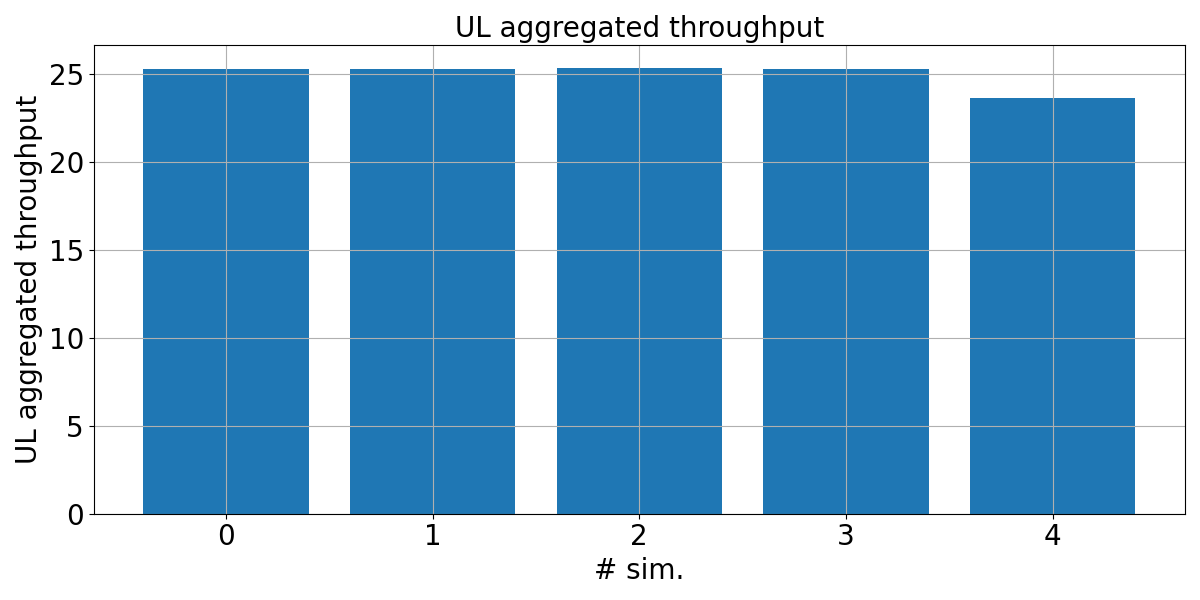
\includegraphics[height=5.0cm]{../comparaciones/validacion_doppler_conjunto2/ue/ul_agg_throughput_multi_sim.png}
		\end{center}
	}
	\end{itemize}
}
\end{itemize}
\end{frame}

% Diapositiva
\begin{frame}
\frametitle{Emulador \textit{FikoRE} - Detalles particulares - Asunciones en la simulación (XII)}

\begin{itemize}
\item {
	Efecto Doppler:
	\begin{itemize}
	\item {
		\begin{center}
		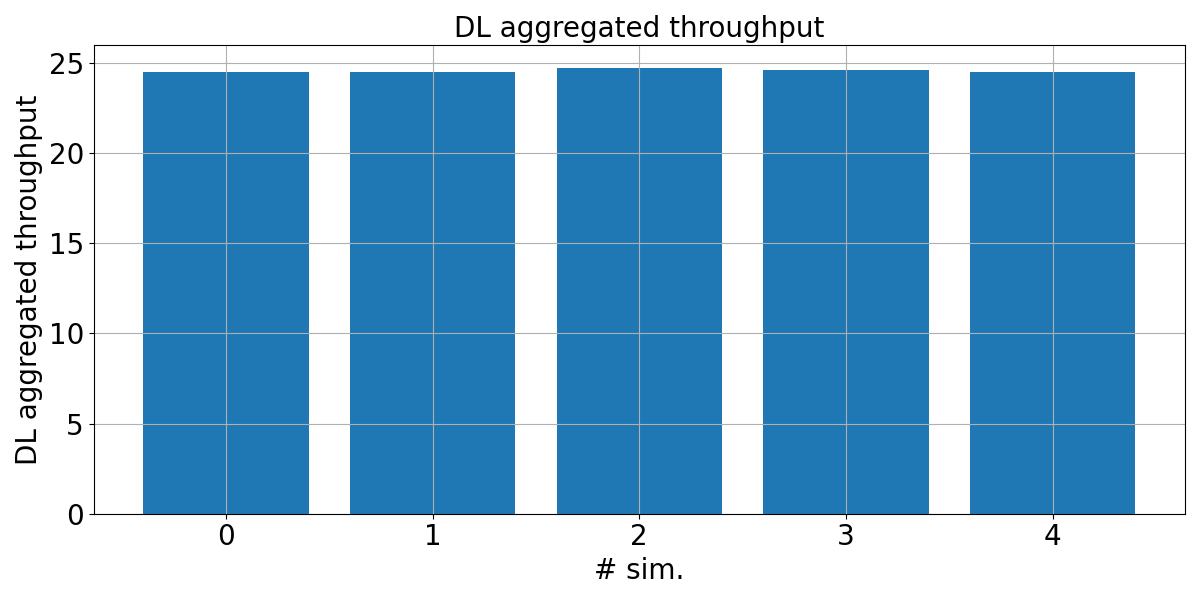
\includegraphics[height=5.0cm]{../comparaciones/validacion_doppler_conjunto2/ue/dl_agg_throughput_multi_sim.png}
		\end{center}
	}
	\end{itemize}
}
\end{itemize}
\end{frame}

% Diapositiva
\begin{frame}
\frametitle{Emulador \textit{FikoRE} - Detalles particulares - Asunciones en la simulación (XIII)}

\begin{itemize}
\item {
	Efecto Doppler:
	\begin{itemize}
	\item {
		\begin{center}
		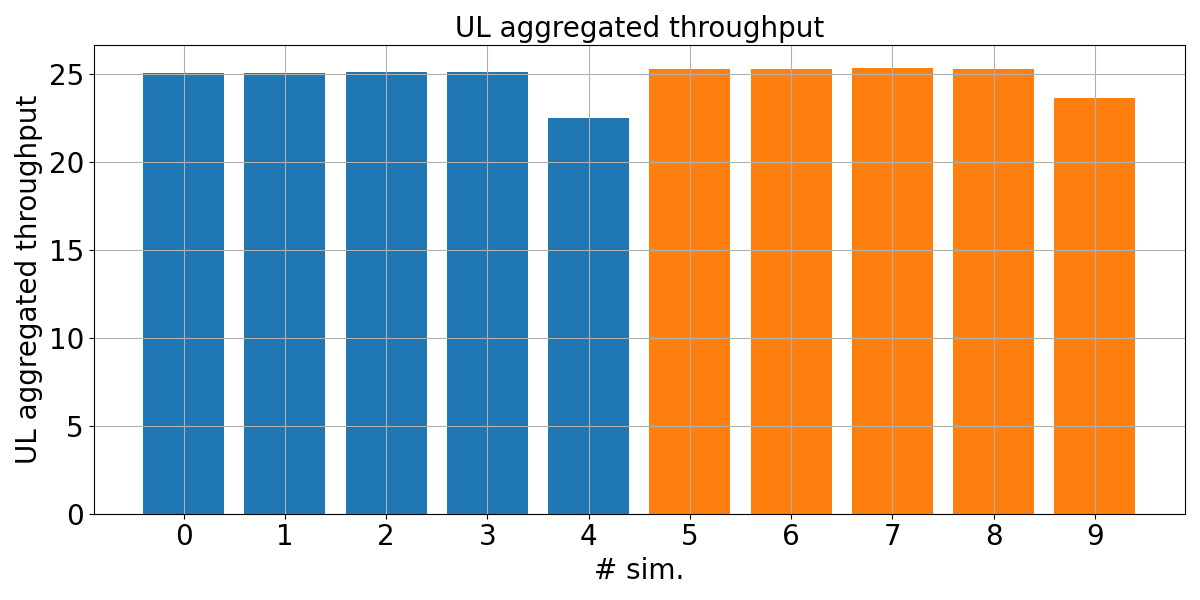
\includegraphics[height=5.0cm]{../comparaciones/validacion_doppler_conjuntos_1_y_2/ue/ul_agg_throughput_multi_sim.png}
		\end{center}
	}
	\end{itemize}
}
\end{itemize}
\end{frame}

% Diapositiva
\begin{frame}
\frametitle{Emulador \textit{FikoRE} - Detalles particulares - Asunciones en la simulación (XIV)}

\begin{itemize}
\item {
	Efecto Doppler:
	\begin{itemize}
	\item {
		\begin{center}
		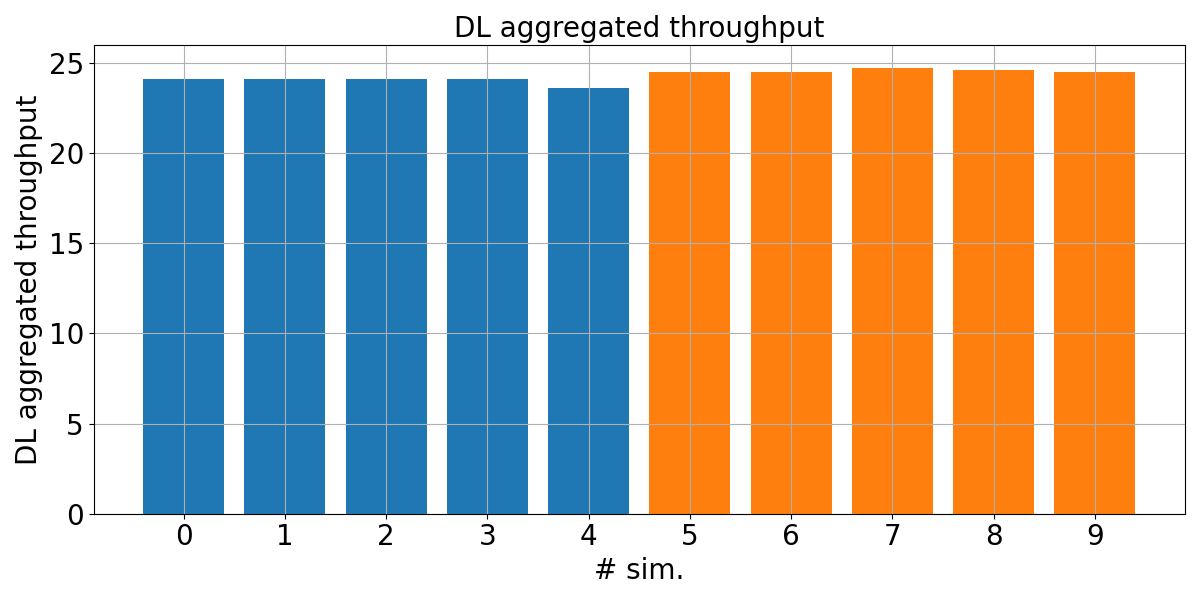
\includegraphics[height=5.0cm]{../comparaciones/validacion_doppler_conjuntos_1_y_2/ue/dl_agg_throughput_multi_sim.png}
		\end{center}
	}
	\end{itemize}
}
\end{itemize}
\end{frame}

% Diapositiva
\begin{frame}
\frametitle{Emulador \textit{FikoRE} - Detalles particulares - Asunciones en la simulación (XV)}

\begin{itemize}
\item {
	Efecto Doppler:
	\begin{itemize}
	\item {
		\begin{center}
		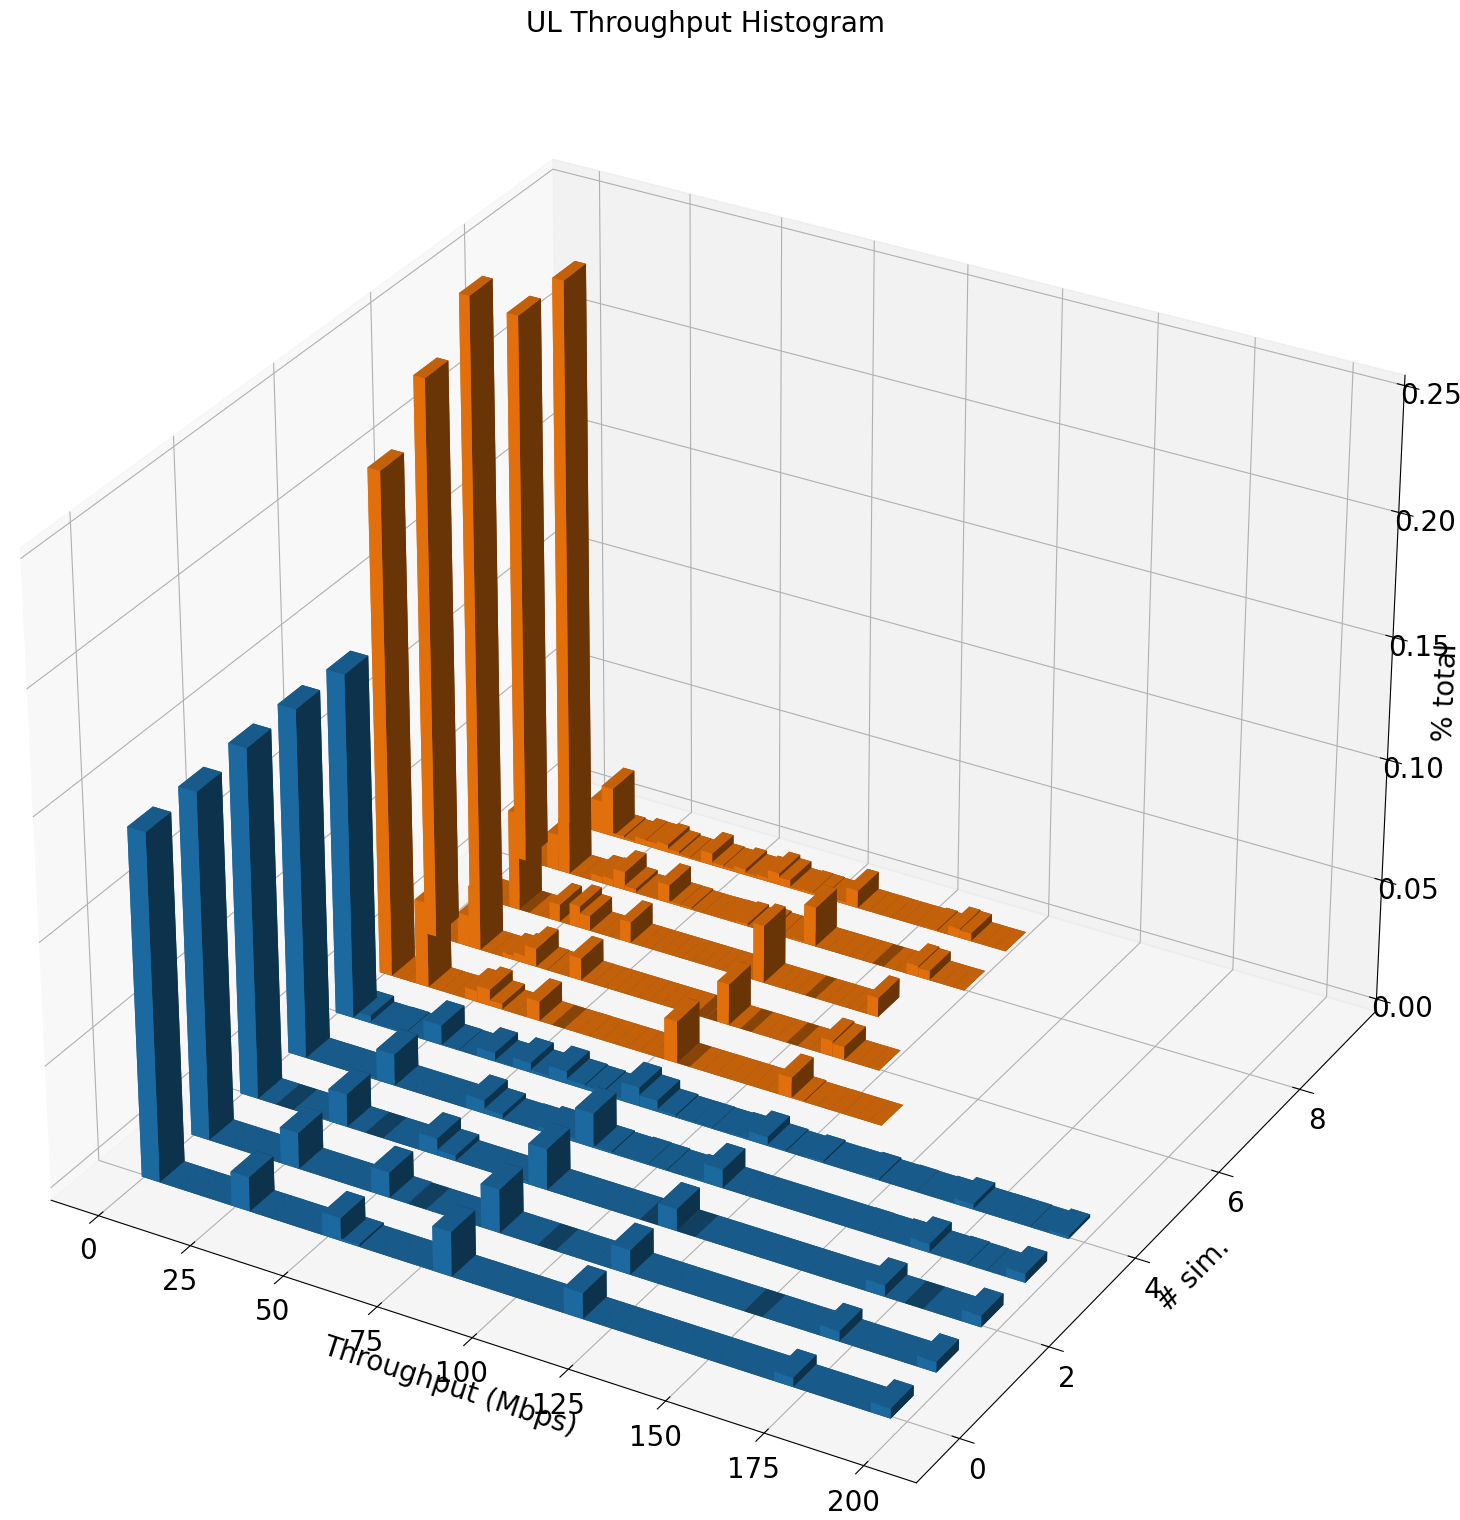
\includegraphics[height=7.0cm]{../comparaciones/validacion_doppler_conjuntos_1_y_2/ue/rul_3d_hist_all_ue_multi.png_cropped.png}
		\end{center}
	}
	\end{itemize}
}
\end{itemize}
\end{frame}

% Diapositiva
\begin{frame}
\frametitle{Emulador \textit{FikoRE} - Detalles particulares - Asunciones en la simulación (XVI)}

\begin{itemize}
\item {
	Efecto Doppler:
	\begin{itemize}
	\item {
		\begin{center}
		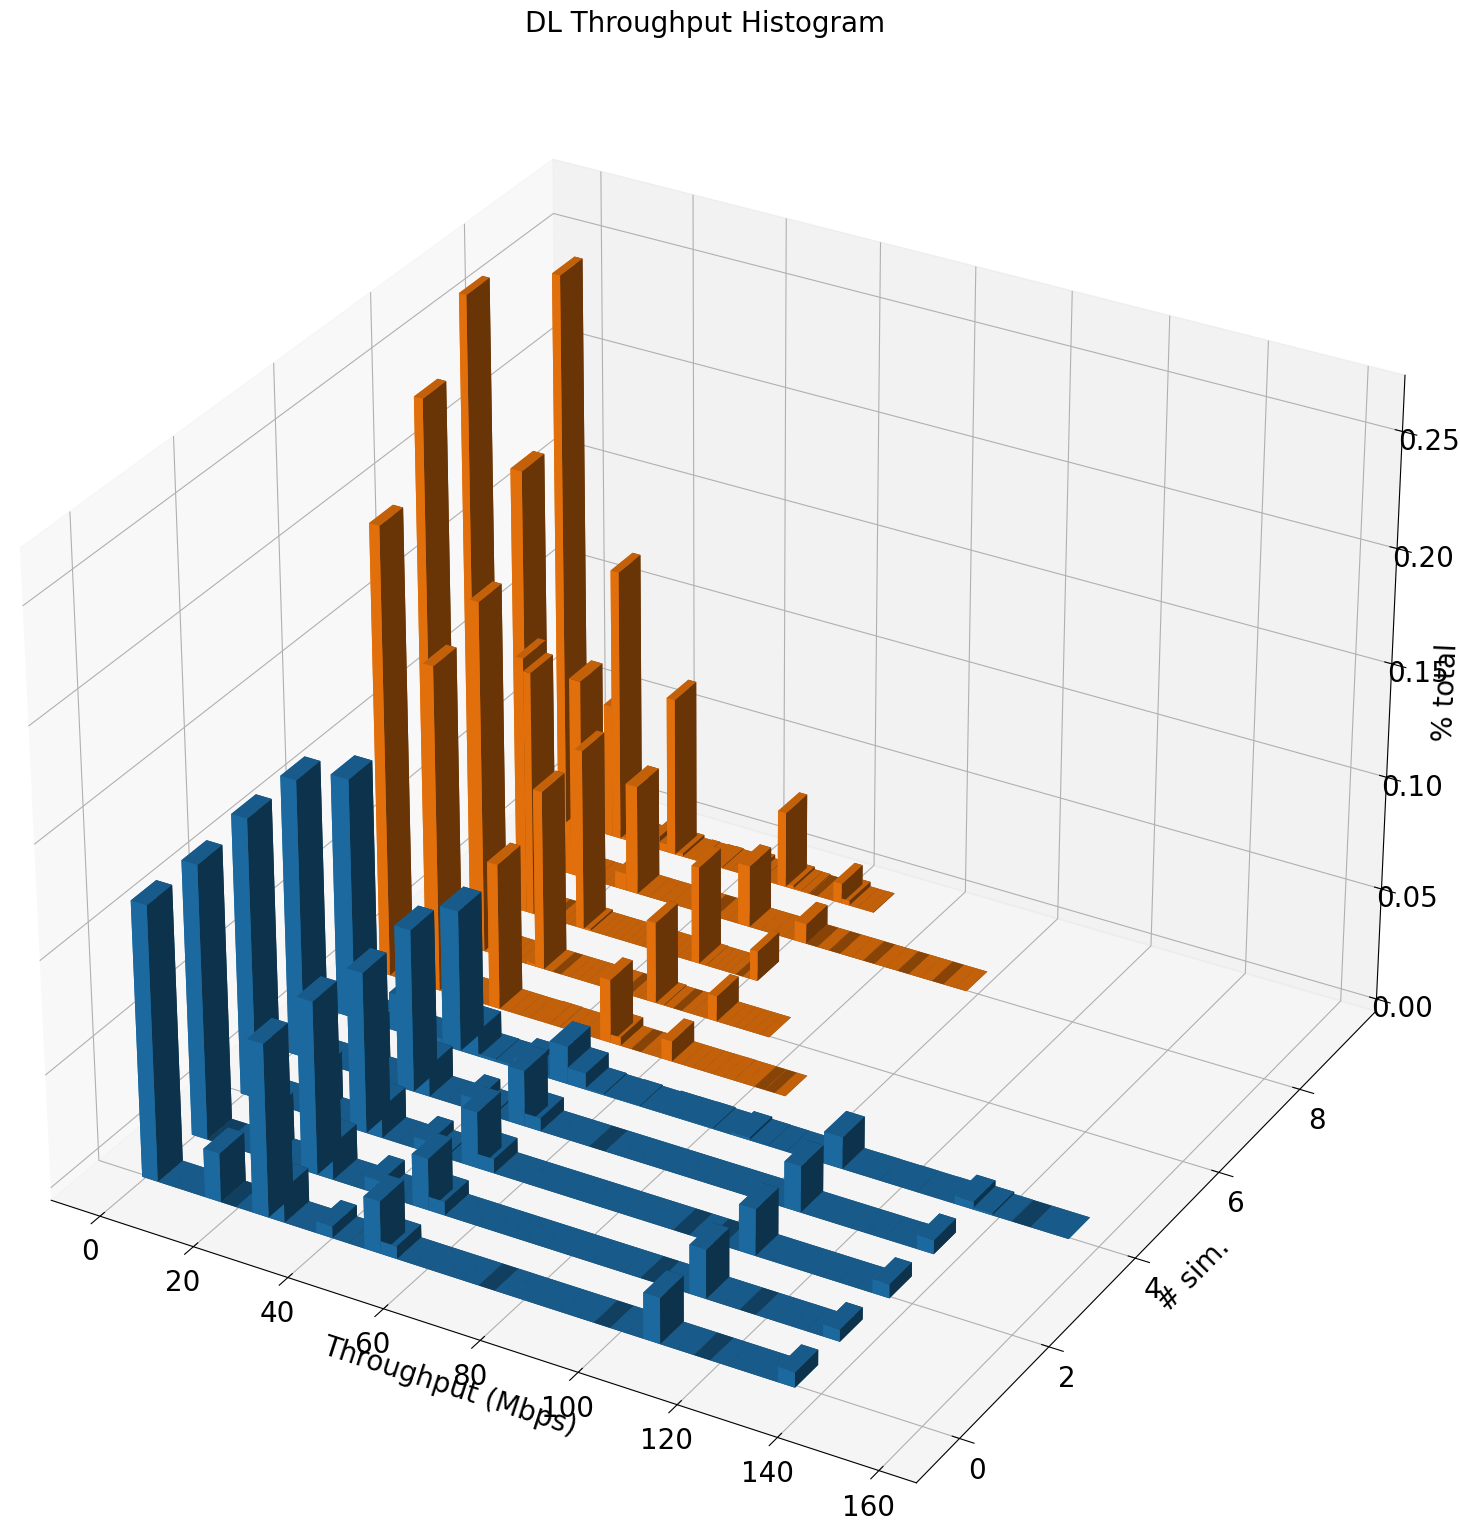
\includegraphics[height=7.0cm]{../comparaciones/validacion_doppler_conjuntos_1_y_2/ue/rdl_3d_hist_all_ue_multi.png_cropped.png}
		\end{center}
	}
	\end{itemize}
}
\end{itemize}
\end{frame}

% Diapositiva
\begin{frame}
\frametitle{Emulador \textit{FikoRE} - Detalles particulares - Asunciones en la simulación (XVII)}

\begin{itemize}
\item {
	Granularidad temporal
	\begin{itemize}
	\item {
		Simulaciones:
		\begin{itemize}
		\item \textit{Validación - Granularidad}
		\end{itemize}
	}
	\item Distinta precisión de la simulación.
	\item Cálculo de los parámetros posible.
	\item Distinta tasa binaria
	\item Mayor tasa, $\rightarrow$ Bloques de menores dimensiones, $\rightarrow$ Evita picos de mayor tasa.
	\end{itemize}
}
\end{itemize}
\end{frame}

% Diapositiva
\begin{frame}
\frametitle{Emulador \textit{FikoRE} - Detalles particulares - Asunciones en la simulación (XVIII)}

\begin{itemize}
\item {
	Granularidad temporal
	\begin{itemize}
	\item {
		\begin{center}
		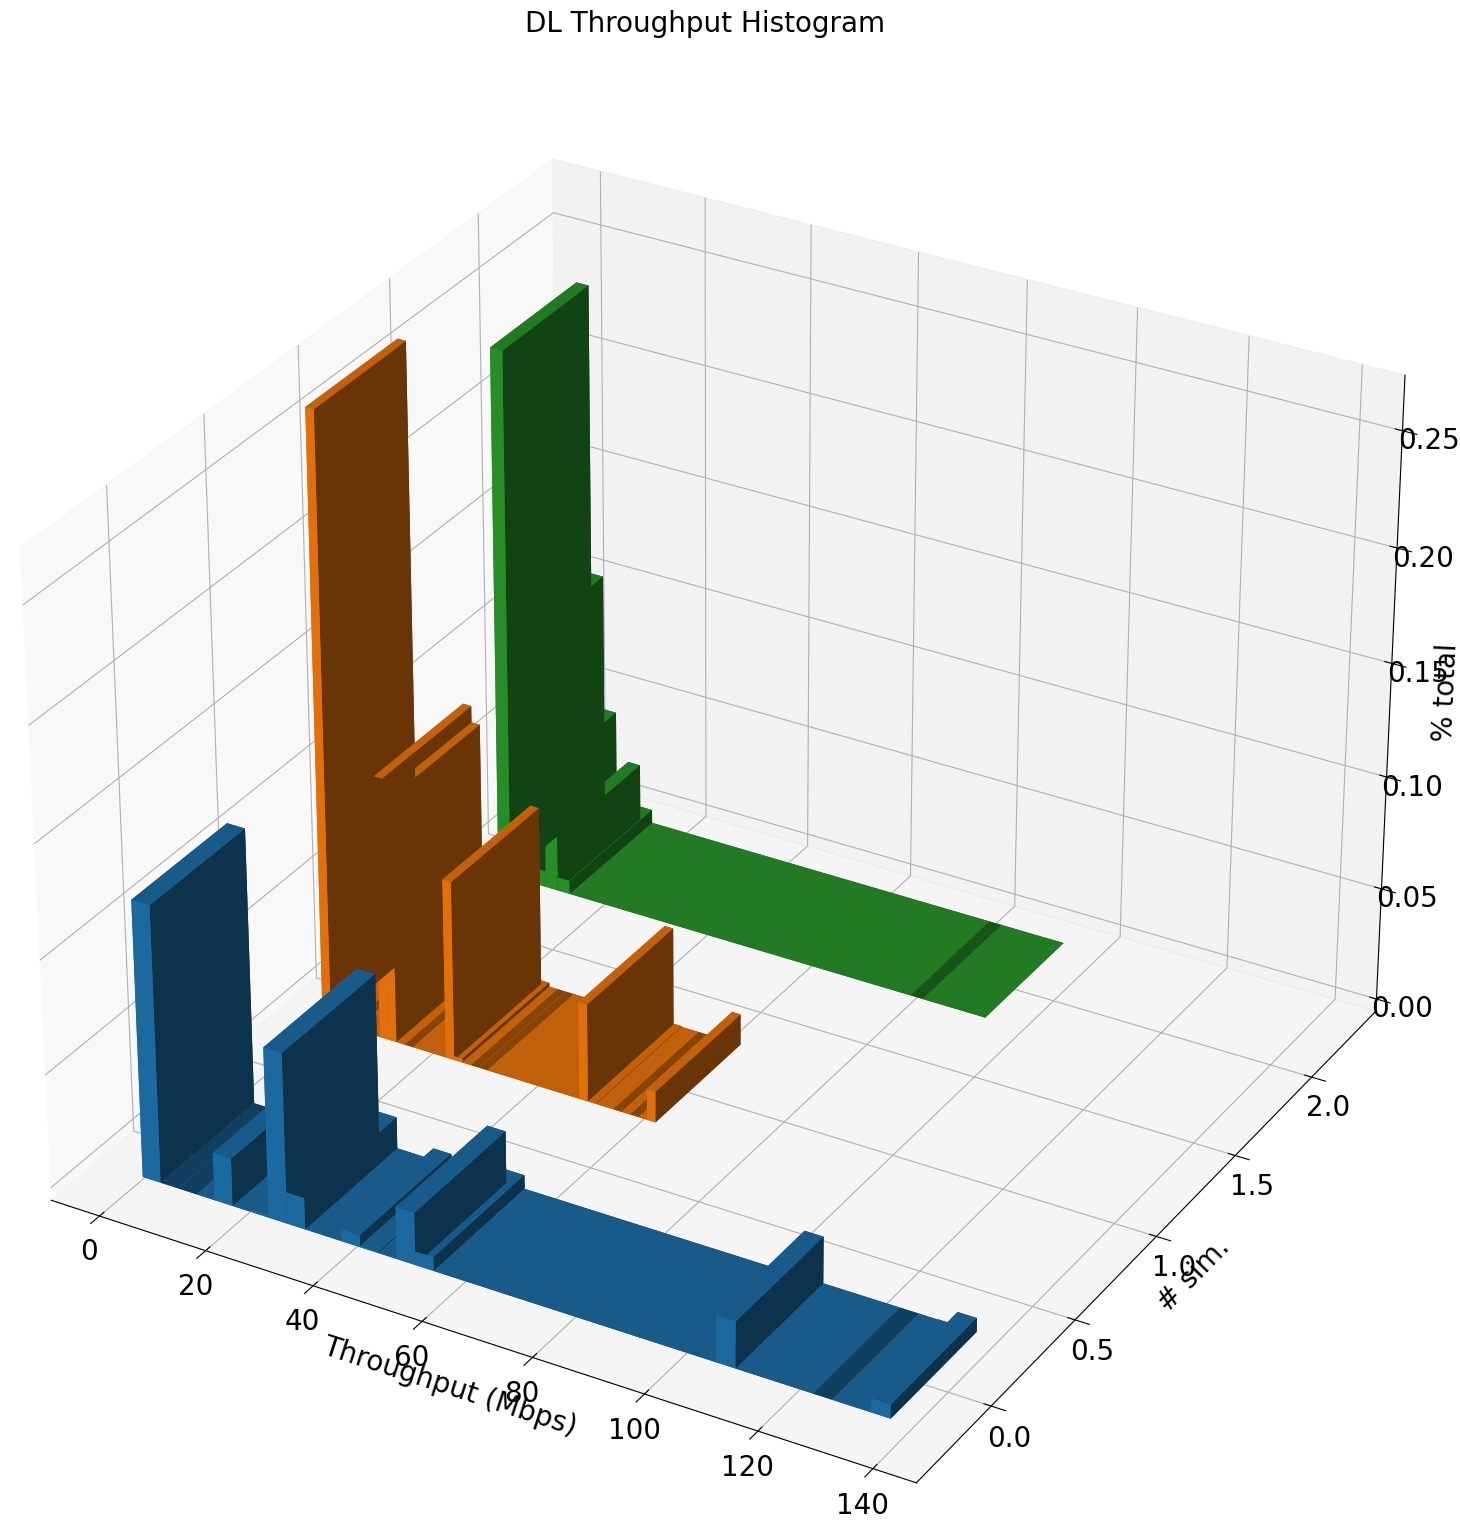
\includegraphics[height=5.0cm]{../comparaciones/validacion_granularidad/ue/rdl_3d_hist_all_ue_multi.png_cropped.png}
		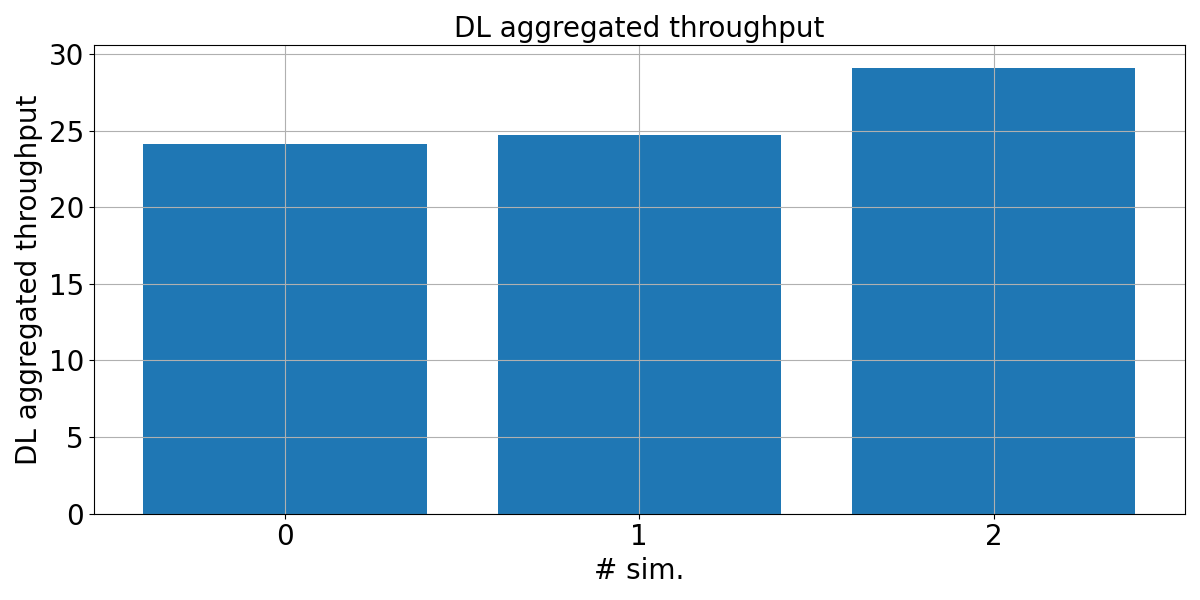
\includegraphics[height=2.5cm]{../comparaciones/validacion_granularidad/ue/dl_agg_throughput_multi_sim.png}
		\end{center}
	}
	\end{itemize}
}
\end{itemize}
\end{frame}





\end{document}

% =============================================================
% =========================== END =============================
% =============================================================

